% bachelor.tex
% Copyright 2016 Zheng Xie <xie.zheng777@gmail.com>
% https://github.com/Tedxz/xjtuthesis-x
%
% This work may be distributed and/or modified under the
% conditions of the LaTeX Project Public License, either version 1.3
% of this license or (at your option) any later version.
% The latest version of this license is in
%   http://www.latex-project.org/lppl.txt
% and version 1.3 or later is part of all distributions of LaTeX
% version 2005/12/01 or later.
%
% This work has the LPPL maintenance status `maintained'.
%
% The Current Maintainer of this work is Zheng Xie.
%
% xjtuthesis-x is a Derived Work of xjtuthesis. The original maintainer of
% xjtuthesis is Weisi Dai (multiple1902 <multiple1902@gmail.com>),
% who published the project on https://code.google.com/p/xjtuthesis/ (no
% longer accessable). Currently, xjtuthesis is maintained by Aetf, and can
% be accessed on https://github.com/Aetf/xjtuthesis.
%
% xjtuthesis-x includes bug fixes, new features and a user guide.
% For detail, please refer to Readme.md.
%
% If you want to contribute to xjtuthesis-x or become the maintainer of
% xjtuthesis-x, please feel free to contact me.

\documentclass[
    bachelor,
    %bigskip, % sets linespread factor to 1.5
    truefont, % just turn it on when using Windows
    %nofont, % remember to manally set the fonts
    pdflinks,
    %colorlinks,
    %compact,
    ]{xjtuthesis}

\graphicspath{{figures/}}


%\input{pages/Latex格式.tex}
\usepackage{amsthm,amsmath,amssymb}

\usepackage{mathrsfs}
\usepackage{boondox-cal}
\usepackage{amsthm,bm}
\usepackage{tikz}
\usetikzlibrary{graphs, positioning, quotes, shapes.geometric}


\usepackage{zhnumber}
%\usepackage{hyperref}

% 生成暗色 pdf
%\usepackage[enable]{darkmode}
%\usepackage{pagecolor}
\usepackage{xcolor}

% Set the background color
\pagecolor{black}

% Set the text color
\color{white}
\usepackage{pdftexcmds}
\usepackage{tcolorbox}
\tcbuselibrary{most}

%C++ 代码显示风格
\usepackage{listings}
\usepackage{algorithm}
\usepackage{xcolor}
\usepackage[dvipsnames]{xcolor}
\lstset{ 
	language=C++,
	backgroundcolor=\color[rgb]{0.96,0.96,0.96},% 背景颜色
	%morekeywords=[2]{nullptr}, % 设置更多的关键字,用逗号分隔
	keywordstyle=[2]\color{blue},
	keywordstyle=\bfseries\color{blue},         % 关键字颜色
	identifierstyle=\color{black},              % 普通标识符颜色
	commentstyle=\color[rgb]{0,0.6,0},          % 注释颜色
	stringstyle=\color[rgb]{0.58,0,0.82},
	basicstyle=\small\ttfamily,        % size of fonts used for the code
	columns=fullflexible,
	breaklines=true,                 % 自动换行
	captionpos=t,                    % sets the caption-position to bottom
	tabsize=4,
	%escapeinside={\%*}{*)},          % if you want to add LaTeX within your code
	emph={self,nullptr,'='}, % 指定强调词,如果有多个,用逗号隔开
	emphstyle=\bfseries\color{Rhodamine}, % 强调词样式设置
	frame=lines, % 边框
	framesep=1em, % 设置代码与边框的距离
	rulesepcolor=\color{red!20!green!20!blue!20},
	numbers=left, % 显示行号在左边
	showstringspaces=false,                     % 不显示字符串内的空格
	%	numbersep=2em, % 设置行号的具体位置
	numberstyle=\footnotesize, % 缩小行号
	extendedchars=false,
	xleftmargin=3em
}


\begin{document}
	
\makeatletter
\newcommand{\ifempty}[1]{\ifnum\pdf@strcmp{#1}{}=\z@}
\makeatother

\newcounter{mytheorem}[section]
\newcounter{mydef}[section]
\newcounter{myproblem}[section]
%\newcounter{special}[part]
%\counterwithin{chapter}{part}
%\numberwithin{figure}{chapter}
%\renewcommand{\thechapter}{第\zhnum{chapter}章}
%\renewcommand{\thesection}{\arabic{chapter}.\arabic{section}}
%\renewcommand{\thesubsection}{\arabic{chapter}.\arabic{section}.\arabic{subsection}}
%\renewcommand{\thesubsubsection}{\arabic{section}.\arabic{subsection}.\arabic{subsubsection}}
\renewcommand{\themydef}{\arabic{section}.\arabic{mydef}}
\renewcommand{\themytheorem}{\arabic{section}.\arabic{mytheorem}}
\renewcommand{\thefigure}{\arabic{chapter}.\arabic{figure}}

\numberwithin{equation}{chapter}
\renewcommand{\theequation}{\arabic{chapter}.\arabic{equation}}
\renewcommand{\t}[1]{\text {#1}}
\setitemize[1]{leftmargin=1.5cm}
%\theoremstyle{definition}
\newtheorem{theorem}[mytheorem]{\indent 定理}
\newtheorem{lemma}[mytheorem]{\indent 引理}
\newtheorem{proposition}[mytheorem]{\indent 命题}
\newtheorem{corollary}[mytheorem]{\indent 推论}
\newtheorem{definition}[mydef]{\indent 定义}
\newtheorem*{definition*}{\indent 定义}
\newtheorem{example}[mytheorem]{\indent 例}
\newtheorem{property}[mytheorem]{\indent 性质}
\newtheorem{remark}[mytheorem]{\indent 注}
\newenvironment{solution}{\begin{proof}[\indent\bf 解]}{\end{proof}}
\renewcommand{\proofname}{\indent\bf 证明}
\def\len{5pt}

%\tcbset{parbox=false,before upper=\par,before lower=\par}
\tcbset{breakable,before upper={\parindent2em},left=0pt,lefttitle=\len, right = 0pt, boxrule = 0.5mm, fonttitle = \bfseries}
\newenvironment{theorem}[1][]{
	\refstepcounter{mytheorem}
	\tcbset{title = {定理\themytheorem \ifempty{#1}\relax\else.(#1)\fi },colback=SeaGreen!10!CornflowerBlue!10,colframe=RoyalPurple!55!Aquamarine!100!}
	\begin{tcolorbox}
}{\end{tcolorbox}}

\newenvironment{lemma}[1][]{
	\refstepcounter{mytheorem}
	\tcbset{title = {引理\themytheorem \ifempty{#1}\relax\else.(#1)\fi },colback=Salmon!20,colframe=Salmon!90!Black}
	\noindent\begin{tcolorbox}
}{\end{tcolorbox}}


\newenvironment{corollary}[1][]{
	\refstepcounter{mytheorem}
	\tcbset{title = {推论\themytheorem \ifempty{#1}\relax\else.(#1)\fi },colback=Emerald!10,colframe=cyan!40!black}
	\noindent\begin{tcolorbox}
}{\end{tcolorbox}}

\newenvironment{proposition}[1][]{
	\refstepcounter{mytheorem}
	\tcbset{title = {},colback=white,colframe=white,colbacktitle=white,coltitle=black}
	\begin{tcolorbox}\noindent\hspace{\len}\textbf{命题\themytheorem.} \ifempty{#1}\relax\else(#1)\fi
}{\end{tcolorbox}}

\newenvironment{example}[1][]{
\refstepcounter{mytheorem}
\tcbset{title = {},colback=white,colframe=white,colbacktitle=white,coltitle=black}
\begin{tcolorbox}\noindent\hspace{\len}\textbf{例\themytheorem.} \ifempty{#1}\relax\else(#1)\fi
}{\end{tcolorbox}}

\newenvironment{property}[1][]{
\refstepcounter{mytheorem}
\tcbset{title = {},colback=white,colframe=white,colbacktitle=white,coltitle=black}
\begin{tcolorbox}\noindent\hspace{\len}\textbf{性质\themytheorem.} \ifempty{#1}\relax\else(#1)\fi
}{\end{tcolorbox}}

\newenvironment{remark}[1][]{
	\refstepcounter{mytheorem}
	\tcbset{title = {},colback=white,colframe=white,colbacktitle=white,coltitle=black}
	\begin{tcolorbox}\noindent\hspace{\len}\textbf{注\themytheorem.} \ifempty{#1}\relax\else(#1)\fi
	}{\end{tcolorbox}}

\newenvironment{remark*}[1][]{
	\tcbset{title = {},colback=white,colframe=white,colbacktitle=white,coltitle=black}
	\begin{tcolorbox}\noindent\hspace{\len}\textbf{注.} \ifempty{#1}\relax\else(#1)\fi
	}{\end{tcolorbox}}

\newenvironment{definition}[1][]{
	\setlength{\parindent}{2em}
	\refstepcounter{mydef}
	\tcbset{title = {定义\themydef\ifempty{#1}\relax\else.(#1)\fi },colback=OliveGreen!10,colframe=Green!70}
	\begin{tcolorbox}
}{\end{tcolorbox}}

\newenvironment{definition*}[1][]{
	\tcbset{title = {定义 \ifempty{#1}\relax\else(#1)\fi },colback=OliveGreen!10,colframe=Green!70}
	\begin{tcolorbox}
	}{\end{tcolorbox}}
\theoremstyle{definition}
%\newtheorem{theorem}[mytheorem]{\indent 定理}
%\newtheorem{lemma}[mytheorem]{\indent 引理}
%\newtheorem{proposition}[mytheorem]{\indent 命题}
%\newtheorem{corollary}[mytheorem]{\indent 推论}
%\newtheorem{definition}[mydef]{\indent 定义}
%\newtheorem*{definition*}{\indent 定义}
%\newtheorem{example}[mytheorem]{\indent 例}
%\newtheorem{property}[mytheorem]{\indent 性质}
%\newtheorem{remark}[mytheorem]{\indent 注}
\newenvironment{solution}{\begin{proof}[\indent\bf 解]}{\end{proof}}
\renewcommand{\proofname}{\indent\bf 证明}

\newenvironment{practice}{
	\practicetrue
	\section*{}
}{\practicefalse}

\newcommand{\problem}[1][]{
	\refstepcounter{myproblem}
	\ifempty{#1}
	\par\arabic{myproblem}.
	\else
	\par#1
	\fi
}

%字体颜色

\newcommand{\tr}[1]{\textcolor{red}{#1}}

%超链接
\newcommand{\hr}[1]{\hyperref[#1]{\t{#1}}}
\newcommand{\hrr}[2][]{\ifempty{#1}\hyperref[#2]{#2}\dotfill\pageref{#2}\else\hyperref[#1]{#2}\dotfill\pageref{#1}\fi}

\newcommand{\set}[2]{\mathbb {#1}^{#2}}
\newcommand{\seta}[2]{\mathbb {#1}_{#2}}
\newcommand{\setb}[3]{\mathbb {#1}^{#2}_{#3}}
\renewcommand{\t}[1]{\text {#1}}
\newcommand{\tb}[1]{\textbf{#1}}

\newcommand{\dps}[1]{\displaystyle {#1}}
\newcommand{\R}{\mathbb R}
\newcommand{\Z}{\mathbb Z}
\newcommand{\C}{\mathbb C}
\newcommand{\N}{\mathbb N}
\newcommand{\Q}{\mathbb Q}

\newcommand{\mydef}[2][]{\label{\ifempty{#1}#2\else #1\fi}\textbf{#2}}
%\newcommand{\mydef}[1]{\label{#1}\textbf{#1}}

%抽象代数

\newcommand{\Aut}{\t {Aut}}  %自同构群
\newcommand{\Inn}{\t {Inn}}  %内自同构群
\newcommand{\Ker}{\t {Ker}}  %核空间
\newcommand{\tIm}{\t {Im}}  %像空间

\newcommand{\Sy}{\t{Sylow} $p$-子群} %Sylow p-子群
\newcommand{\lAbel}{有限 \t{Abel}\ }
\newcommand{\Abel}{\t{Abel}\ }
\newcommand{\rad}{\t{rad}\ }

% 数学分析

\newcommand\mint[1][]{\dps\int_{\hspace{-0.4em} #1}}
\newcommand{\ti}{\t i}
\newcommand{\td}{\ \t d}
\newcommand{\fly}{\t{Fourier}\ }
\newcommand{\lpxc}{\t{Lipschitz}\ 条件}

%常微分方程
\newcommand{\wfen}[3][]{\dfrac{\td #2^{#1}}{\td^{#1} #3}}
\newcommand{\pfen}[3][]{\dfrac{\partial #2^{#1}}{\partial^{#1} #3}}


    % 请修改 meta.tex 中的论文元信息
    % meta.tex
% Copyright 2016 Zheng Xie <xie.zheng777@gmail.com>
% https://github.com/Tedxz/xjtuthesis-x
%
% This work may be distributed and/or modified under the
% conditions of the LaTeX Project Public License, either version 1.3
% of this license or (at your option) any later version.
% The latest version of this license is in
%   http://www.latex-project.org/lppl.txt
% and version 1.3 or later is part of all distributions of LaTeX
% version 2005/12/01 or later.
%
% This work has the LPPL maintenance status `maintained'.
%
% The Current Maintainer of this work is Zheng Xie.
%
% xjtuthesis-x is a Derived Work of xjtuthesis. The original maintainer of
% xjtuthesis is Weisi Dai (multiple1902 <multiple1902@gmail.com>),
% who published the project on https://code.google.com/p/xjtuthesis/ (no
% longer accessable). Currently, xjtuthesis is maintained by Aetf, and can
% be accessed on https://github.com/Aetf/xjtuthesis.
%
% xjtuthesis-x includes bug fixes, new features and a user guide.
% For detail, please refer to Readme.md.
%
% If you want to contribute to xjtuthesis-x or become the maintainer of
% xjtuthesis-x, please feel free to contact me.

% 标题,中文
\ctitle{课程资料整理}

% 作者,中文
\cauthor{数学强基 2301 刘欣楠}

% 学科,中文,本科生不需要
\csubject{}

% 导师姓名,中文
\csupervisor{李四}

% 关键词,中文。用全角分号「;」分割
% 研究生的应首先从《汉语主题词表》中摘选
\ckeywords{数学专业课、专业基础课、知识点、作业}

% 提交日期,本科生不需要
\cproddate{\the\year 年\the\month 月}

% 论文类型,中文,本科生不需要
% 从理论研究、应用基础、应用研究、研究报告、软件开发、设计报告、案例分析、调研报告、其它中选择
\ctype{}

% 论文标题,英文
\etitle{}

% 作者姓名,英文
\eauthor{}

% 学科,英文,本科生不需要
\esubject{}

% 导师姓名,英文
\esupervisor{}

% 关键词,英文。用半角分号和一个半角空格「; 」分割
\ekeywords{Wikipedia; Free encyclopedia; Winner; Good morning}

% 学科门类,英文
% 从Philosophy(哲学)、Economics(经济学)、Law(法学)、Education(教育学)、Arts(文学)、
%   Science(理学)、Engineering Science(工学)、Medicine(医学)、Management Science(管理学)中选择
\ecate{}

% 提交日期,英文,本科生不需要
% 应当和 cproddate 保持一致
\eproddate{\monthname{\month}\ \the\year}

% 论文类型,英文,本科生不需要
% 从Theoretical Research(理论研究)、Application Fundamentals(应用基础)、Applied Research(应用研究)、
%   Research Report(研究报告)、Software Development(软件开发)、Design Report(设计报告)、
%   Case Study(案例分析)、Investigation Report(调研报告)、其它(Other)中选择
\etype{}

% 摘要,中文。段间空行
\cabstract{
}

% 摘要,英文。段间空行
\eabstract{
}


    \xjtucinfopage
    \xjtueinfopage
    \xjtutoc
    \clearpage



    % 主要符号表,可以没有
    %% multiple1902 <multiple1902@gmail.com>
% denotation.tex
% Copyright 2011~2012, multiple1902 (Weisi Dai)
% https://code.google.com/p/xjtuthesis/
% 
% It is strongly recommended that you read documentations located at
%   http://code.google.com/p/xjtuthesis/wiki/Landing?tm=6
% in advance of your compilation if you have not read them before.
%
% This work may be distributed and/or modified under the
% conditions of the LaTeX Project Public License, either version 1.3
% of this license or (at your option) any later version.
% The latest version of this license is in
%   http://www.latex-project.org/lppl.txt
% and version 1.3 or later is part of all distributions of LaTeX
% version 2005/12/01 or later.
%
% This work has the LPPL maintenance status `maintained'.
% 
% The Current Maintainer of this work is Weisi Dai.
%




    \xjtucontent

	%	\chapter{高等代数}

\input{pages/高等代数/线性空间}
\input{pages/高等代数/有限维线性空间}
\input{pages/高等代数/线性空间的运算}
\input{pages/高等代数/线性映射}
\input{pages/高等代数/线性映射矩阵表示}
\input{pages/高等代数/矩阵运算基础}
\input{pages/高等代数/相抵标准形}
\input{pages/高等代数/矩阵运算进阶}
\input{pages/高等代数/有限域上的矩阵}
\input{pages/高等代数/商与对偶}
\input{pages/高等代数/多重线性映射与张量计算}
\input{pages/高等代数/行列式}
\input{pages/高等代数/矩阵空间}
\input{pages/高等代数/线性方程组}
\input{pages/高等代数/线性同余方程与纽结}
\input{pages/高等代数/多项式}
\input{pages/高等代数/控制法及其在矩阵理论中的应用}
\input{pages/高等代数/相似标准形}
\input{pages/高等代数/若当标准形}
\input{pages/高等代数/多项式的进一步讨论}
\input{pages/高等代数/有理标准形}
\input{pages/高等代数/对称多项式和Young图}
\input{pages/高等代数/内积空间}
\input{pages/高等代数/内积空间上的算子}
\input{pages/高等代数/希尔伯特空间引论}
\input{pages/高等代数/奇异值分解}
\input{pages/高等代数/高等代数与几何}
\input{pages/高等代数/二次型}
\input{pages/高等代数/射影几何的代数方法}
\input{pages/高等代数/有限域上的二次型}
\input{pages/高等代数/二次型几何}
\input{pages/高等代数/线性空间}
\input{pages/高等代数/实数域的扩域}
\input{pages/高等代数/线性动力系统}
\input{pages/高等代数/线性代数与微积分}
\input{pages/高等代数/范畴论视角下的线性代数}



		\newpage
\inmainbodyfalse
\part{抽象代数}\label{抽象代数}
\chaptermark{抽象代数}
这部分内容主要参考丘维声《近世代数》\cite{丘维声2015近世代数}


\begin{denotation}{抽象代数定义及主要定理}
	\item[$R$]    \hrr[环]{环}
	\item[$a^{-1}$] \hrr[单位]{可逆元、单位}
	\item[] \hrr{单位群}
	\item[]    \hrr[零因子]{\t{零因子}}
	\item[$F$] \hrr[域]{域}
	\item[$G$] \hrr[群]{群}
	
	%
	\item[$\langle a\rangle$] \hrr[循环群]{循环群}
	\item[$|a|$] \hrr[元素的阶]{元素的阶}
	\item[$F^*$] \hrr[F*]{$F^*$}
	\item[]    \hrr[群作用]{\t{群作用}}
	\item[]    \hrr[作用的核]{\t{作用的核}}
	\item[]    \hrr[忠实的作用]{\t{忠实的作用}}
	\item[$Z(G)$]    \hrr[中心]{\t{中心}}
	\item[]    \hrr[自同构]{\t{自同构, 内自同构}}
	\item[\Aut]    \hrr[自同构]{\t{自同构群}}
	\item[\Inn]    \hrr[自同构]{\t{内自同构群}}
	\item[$G(x)$]    \hrr[轨道]{\t{轨道, 完全代表系}}
	\item[$G_x$]    \hrr[稳定子群]{\t{稳定子群}}
	\item[]    \hrr[轨道-稳定子定理]{\t{轨道-稳定子定理}}
	\item[$G(x)$]    \hrr[共轭类]{\t{共轭类}}
	\item[]    \hrr[类方程]{\t{类方程}}
	\item[$C_G(x)$]    \hrr[中心化子]{\t{中心化子}}
	\item[]    \hrr[齐性空间]{\t{作用的传递, 齐性空间}}
	\item[$F(g)$]    \hrr[不动点集]{\t{不动点集}}
	\item[]		\hrr[Burnside]{\t{Burnside 引理}}
	\item[$\Omega_0$]    \hrr[不动点]{\t{作用的不动点, 不动点集}}
	\item[$|G|=p^m$]    \hrr[p-群]{$p$\t{-群}}
	\item[]    \hrr[Sylow1]{\t{Sylow 第一定理}}
	\item[]    \hrr[Sylow2]{\t{Sylow 第二定理}}
	\item[]    \hrr[Sylow3]{\t{Sylow 第三定理}}
	\item[]    \hrr[四元数]{\t{四元数}}
	
	%
	\item[]    \hrr[环同态]{\t{环同态}}
	\item[$I$]    \hrr[理想]{\t{理想}}
	\item[]    \hrr[单环]{\t{单环}}
	\item[]    \hrr[左理想]{\t{左理想}}
	\item[$R/I$]    \hrr[商环-同余类]{\t{商环, 同余类}}
	\item[$\pi:R\to R/I$]    \hrr[自然环同态]{\t{自然环同态}}
	\item[]    \hrr[环同态基本定理]{\t{环同态基本定理}}
	\item[]    \hrr[第一环同构定理]{\t{第一环同构定理}}
	\item[]    \hrr[第二环同构定理]{\t{第二环同构定理}}
	\item[$(S)$]    \hrr[由S生成的理想]{\t{由 $S$ 生成的理想}}
	\item[$(a)$]    \hrr[主理想]{\t{主理想}}
	\item[$I+J,IJ$]    \hrr[理想的运算]{\t{理想的运算}}
	\item[$I+J=R$]    \hrr[理想的互素]{\t{理想的互素}}
	\item[$a\equiv b(\bmod I)$]    \hrr[环的同余]{\t{同余}}
	\item[]    \hrr[中国剩余定理]{\t{中国剩余定理}}
	\item[$\rad\ I$]    \hrr[理想的根]{理想的根}
	\item[]    \hrr[幂零元]{幂零元、幂零根}
	\item[]    \hrr[理想的内直和]{理想的内直和}
	\item[]    \hrr[整环]{整环}
	\item[$P$]    \hrr[素理想]{素理想}
	\item[$M$]    \hrr[极大理想]{极大理想}
	\item[]    \hrr[环的特征]{环的特征}
	\item[]  \hrr[扩环]{扩环}
	\item[] \hrr[域扩张]{扩域、域扩张、子域}
	\item[$R{[\widetilde{\alpha}]}$] \hrr[元素生成的子环]{元素生成的子环}
	\item[$a_0+a_1\widetilde{\alpha}+\cdots+a_n\widetilde{\alpha}^n$] \hrr[元素在R上的多项式]{元素在 $R$ 上的多项式}
	\item[] \hrr[超越元]{超越元、代数元、极小多项式}
	\item[] \hrr[代数数]{超越数、代数数}
	\item[$\Q{[\xi_n]}$] \hrr[分圆域]{分圆域}
\end{denotation}

\newpage

%\renewcommand{\thechapter}{}
\chapter*{绪论}
\chaptermark{绪论}
%\renewcommand{\thechapter}{第\zhnum{chapter}章}

\addcontentsline{toc}{chapter}{绪论}



\begin{definition}\label{环}
	设 $R$ 是一个非空集合, 在其上定义加法和乘法, 若满足下列性质
	\begin{itemize}[leftmargin=1.5cm]
		\item[(1)](加法交换律) $a+b=b+a,\forall\ a,b\in R$.
		\item[(2)](加法结合律) $(a+b)+c = a+(b+c),\forall\ a,b,c\in R$.
		\item[(3)] 存在\textbf{零元}, 记作 $0$.
		\item[(4)] 存在\textbf{负元}, 记作 $-a$.
		\item[(5)](乘法结合律) $(ab)c=a(bc),\forall\ a,b,c\in R$.
		\item[(6)](乘法分配律) $a(b+c)=ab+ac,(b+c)a=ba+ca$.
	\end{itemize}
	则称 $R$ 是一个\textbf{环}.
\end{definition}

\begin{definition}\label{环的单位元}
	如果环 $R$ 中有一个元素 $e$ 具有下述性质: $$ea=ae=a,\quad\forall a\in R,$$ 那么称 $e$ 是 $R$ 的\textbf{单位元}, 并称 $R$ 是幺环.
\end{definition}

\begin{definition}
	设 $R$ 是幺环. 对于 $a\in R$,  如果存在 $b\in R$ 使得 $$ab=ba=e$$, 那么称 $a$ 是一个\mydef{可逆元}(或\mydef{单位}), $b$ 称作 $a$ 的\mydef{逆元}, 记作 $a^{-1}$.
\end{definition}

\begin{definition}
	幺环 $R$ 的所有\hr{单位}关于 $R$ 上的乘法构成一个群, 称之为 $R$ 的\mydef{单位群}.
\end{definition}

\begin{definition}\label{零因子}
	设 $R$ 是一个环. 对于 $a\in R$, 如果存在 $c\in R$ 且 $c\neq 0$, 使得 $ac=0$(或 $ca=0$), 那么称 $a$ 是一个\textbf{左零因子}(或\textbf{右零因子}). 二者统称\textbf{零因子}.
\end{definition}


\begin{definition}\label{域}
	设 $F$ 是交换幺环, 如果 $F$ 中每个非零元素都是可逆元, 那么称 $F$ 是一个\textbf{域}.
\end{definition}

\begin{definition}\label{群}
	设 $G$ 是一个非空集合. 如果在 $G$ 上定义了一个代数运算, 通常称作乘法, 并且满足:
	\begin{itemize}[leftmargin=1.5cm]
		\item[(1)] $(ab)c=a(bc),\ \forall\ a,b,c\in G$ (结合律);
		\item[(2)] $G$ 中存在单位元 $e$.
		\item[(3)] $G$ 中每个元素都可逆.
	\end{itemize}
	那么称 $G$ 是一个\textbf{群}.
\end{definition}

\begin{definition}
	当群 $G$ 中只有有限个元素时, 称 $G$ 为\textbf{有限群}, 且元素个数称为 $G$ 的阶, 记作 $|G|$. 否则称 $G$ 是\textbf{无限群}.
\end{definition}

\begin{remark*}
	只有有限阶群才有群的阶, 做题时要注意题设条件.
\end{remark*}
\inmainbodytrue

\chapter{群}

\section{循环群}

\begin{definition}
	设 $G$ 是一个群, 如果 $G$ 的每一个元素都能写成 $G$ 的某个元素 $a$ 的整数次幂的形式, 那么称 $G$ 为\mydef{循环群}, 称 $a$ 是 $G$ 的一个\textbf{生成元}, 并记 $G=\langle a\rangle$.
\end{definition}

\begin{definition}\label{元素的阶}
	对于群 $G$ 中元素 $a$, 如果存在最小的正整数 $n$, 使得 $a^n=e$. 则称 $a$ 的\textbf{阶}为 $n$, 记作 $|a|=n$. 如果不存在这样的 $n$, 则称 $a$ 是\textbf{无限阶元素}.
\end{definition}

\begin{proposition}
	有限群 $G$ 是循环群, 当且仅当 $\exists\ a\in G,\ s.t.\  |a| = |G|$.
\end{proposition}

\begin{proposition}
	设 $a\in G,\ |a|=n$ 则 $$a^m = e\Leftrightarrow n\mid m.$$
\end{proposition}

\begin{proposition}
	设 $a\in G,\ |a|=n$ 则 $$|a^k|=\frac n {(n,k)}.$$
\end{proposition}

\begin{proposition}
	若 $a,b\in G,\ ab=ba,\ |a|=n,|b|=m, (n,m)=1$ 则 $|ab|=nm$.
\end{proposition}

\begin{proposition}
	设 $G$ 是\lAbel 群, 则 $\exists\ a\in G,\ s.t.\ \forall b \in G,|b|\big| |a|$.
\end{proposition}

\begin{theorem}
	设 $m$ 是大于 $1$ 的整数, 则 $\Z_m^*$ 为循环群当且仅当 $m$ 为下列情形之一: $$2,\ 4,\ p^r,\ 2p^r,\quad \t{其中}\ p\ \t{是奇素数},\ r\in\N^*$$
\end{theorem}

\begin{theorem}\label{F*}
	有限域 $F$ 的所有非零元组成的集合 $F^*$ 对于乘法构成群, 且是循环群.
\end{theorem}

\begin{definition}
	群同构
\end{definition}

\begin{proposition}
	设 $\sigma$ 是 $G$ 到 $\widetilde{G}$ 的一个\hr{群同构映射}, 则
	\begin{itemize}[leftmargin=1.5cm]
		\item[(1)] $\sigma(e)=\widetilde{e}$.
		\item[(2)]$\sigma(a^{-1})=\sigma(a)^{-1}$.
		\item[(3)]$\sigma(a)$ 与 $a$ 的阶相同.
	\end{itemize}
\end{proposition}


\begin{theorem}
	\begin{itemize}
		\item[(1)] 任意一个无限循环群都与 $(\Z,+)$ 同构;
		\item[(2)] 对于 $m>1$, 任意一个 $m$ 阶循环群都与 $(\Z_m,+)$ 同构;
		\item[(3)] $1$ 阶循环群都与加法群 $\{0\}$ 同构.
	\end{itemize}
\end{theorem}

\begin{theorem}
	设 $m_1,m_2$ 是大于 $1$ 的整数, 则 $(\Z_{m_1}\oplus\Z_{m_2},+)$ 是循环群当且仅当 $(m_1,m_2)=1$.
\end{theorem}

\begin{practice}
	\problem 证明: 若 $\Z_m^*$ 是循环群, 则 $\Z_m^*$ 的生成元个数等于 $\varphi(\varphi(m))$.
	\begin{proof}
		$|\Z_m^*|=\varphi(m)$, 设 $a$ 是 $\Z_m^*$ 的生成元, 那么 $|a|=\varphi(m)$.
		\\则有 $b=a^k\in\Z_m^*$ 是生成元 $\Leftrightarrow |a^k|=\varphi(m)\Leftrightarrow \dfrac{\varphi(m)}{(\varphi(m),k)}\Leftrightarrow(\varphi(m),k)=1$.
	\end{proof}

	\problem 证明: 如果群 $G$ 的阶为偶数, 那么 $G$ 必有 $2$ 阶元.
	\begin{proof}
		反设 $G$ 中没有 $2$ 阶元, 则对于 $G$ 中每个个非单位元 $a$ 都有 $a\neq a^{-1}$. 从而可以将 $G$ 的元素和对应的逆元两两配对, 也即除去单位元后元素个数为偶数, 所以总个数为奇数矛盾. 故 $G$ 中有 $2$ 阶元.
	\end{proof}
\end{practice}

\section{图形的对称(性)群}

\begin{definition}
	平面上(或空间中)的一个变换 $\sigma$ 如果保持任意两点的距离不变, 那么称 $\sigma$ 是平面上(或空间中)的一个\mydef{正交点变换}(或\mydef{保距变换})(isometry).
\end{definition}

\begin{definition}
	平面上(或空间中)的一个正交点变换 $\sigma$ 如果使得图形 $\Gamma$ 的像与自身重合, 那么称 $\sigma$ 是图形 $\Gamma$ 的\mydef[对称变换]{对称(性)变换}.

	容易验证, $\Gamma$ 的所有对称变换构成一个群, 称为\mydef[对称群]{图形 $\Gamma$  的对称(性)群}.
\end{definition}

我们一般用 $\tau$ 来表示图形关于直线反射(轴对称)的对称变换, 用 $\sigma$ 来表示关于图形中心旋转得到的对称变换.

用 $D_n$ 表示正 $n$ 边形的对称群.

当 $n=4$ 时, 正方形一共有四条对称轴对应 $\tau_1,\tau_2,\tau_3,\tau_4$, 且每转动 $90^\circ$ 都重合对应着 $\sigma,\sigma^2,\sigma^3,\sigma_4=I$.

经过研究, $D_4=\{I,\sigma,\sigma^2,\sigma^3,\tau_1,\tau_2,\tau_3,\tau_4\}$. 同时 $\tau_i$ 也可以由 $\sigma$ 和 $\tau_1$ 表示. 所以也可以把 $D_4$ 简单的记作 $$D_4=\langle \sigma,\tau|\sigma^4=\tau^2=I,(\tau\sigma)^2=I\rangle.$$

类似的, 对于 $D_n$ 也可以记作 $\langle \sigma,\tau|\sigma^n=\tau^2=(\tau\sigma)^2=I\rangle$.

由于 $\tau\sigma=\sigma^{-1}\tau=\sigma^{n-1}\tau\neq\sigma\tau$, 所以 $D_n$ 是非 \Abel 群.

我们称 $D_n$ 为\mydef{二面体群}, 且有 $|D_n|=2n$.

\section{$n$ 元对称群}

\begin{definition}
	对于非空集合 $\Omega$, 设 $S_\Omega$ 是全部 $\Omega$ 到自身的双射构成的集合, 容易验证 $S_\Omega$ 是一个群, 我们称之为\mydef{全变换群}(full transformationm group).

	特别的, 当 $\Omega$ 是有限集合时, 称 $\Omega$ 到自身的双射为 $\Omega$ 上的一个\mydef{置换} (permutation). 当 $|\Omega|=n$ 时, 称 $\Omega$ 上的置换为 \textbf{$n$ 元置换}, 并称 $S_\Omega$ 为 \textbf{$n$ 元对称群}, 记作 $S_n$.
\end{definition}

\begin{definition}
	如果一个 $n$ 元置换 $\sigma$ 把 $i_1$ 映成 $i_2$, 把 $i_2$ 映成 $i_3$,$\cdots$, 把 $i_{r}$ 映成 $i_1$, 并且保持其余元素不变, 那么称 $\sigma$ 为 $r-$\textbf{轮换}, 简称为\mydef{轮换}, 记作 $(i_1i_2i_3\cdots i_{r-1}i_r)$.

	特别地, 当 $r=2$ 时, 也称为\mydef{对换}. 恒等映射 $I$ 记作 $(1)$.

	如果两个轮换之间没有公共元素, 则称它们\mydef[轮换不相交]{不相交}.
\end{definition}

\begin{property}
	\begin{equation}
		(i_1i_2\cdots i_{r-1} i_r)^{-1}=(i_ri_{r-1}\cdots i_2i_1).
	\end{equation}
	\begin{equation}
		(i_1i_2\cdots i_{r-1}i_r)=(i_1i_r)(i_1i_{r-1})\cdots(i_1i_3)(i_1i_2).
	\end{equation}
	\begin{equation}\label{eq:对称群:3}
		(ij)=(1i)(1j)(1i).
	\end{equation}
\end{property}

\begin{theorem}
	 $S_n$ 中任一非单位元的置换都能表示成一些两两不相交的轮换的乘积, 并且除了轮换的排列次序外, 表示法是唯一的.
\end{theorem}

\begin{remark*}
	在计算多个轮换复合时, 注意运算顺序是从右至左,  因为轮换本质上是函数映射的复合.
\end{remark*}



\begin{corollary}\label{coro:对称群:1}
	 $S_n$ 中每个置换都可以表示成一些对换的乘积.
\end{corollary}

\begin{proposition}
	$S_n$ 中一个置换表示成对换的乘积, 其中对换的个数的奇偶性只和这个置换本身有关, 与表示方式无关.
\end{proposition}

\begin{example}(\href{https://qoj.ac/contest/1865/problem/9801}{$49^{th}\ \t{ICPC Asia Shenyang Regional Contest D.Dot Product Game}$})

	当我们将 $b_i$ 映射到 $1\sim n$ 时, 每次操作都会改变 $a_i$ 对换数目的奇偶性, 而最终状态是 $a_i$ 也变为 $1\sim n$, 所以只需计算初始的奇偶性就可以判断.
\end{example}

\begin{definition}
	基于上述命题, 我们将可以由偶数个对换表示的置换称为\mydef{偶置换}, 由奇数个对换表示的置换称为\mydef{奇置换}.

	同时, 按照定义偶置换和偶置换的乘积还是偶置换, 所以所有偶置换对乘法封闭是 $S_n$ 的子群, 称为 \mydef[n元交错群]{$n$ 元交错群}, 记作 $A_n$. 且有 $|A_n|=\dfrac 1 2 |S_n|=\dfrac{n!} 2$.
\end{definition}

\begin{definition}
	设 $S$ 的群 $G$ 的一个非空子集, 如果 $G$ 中每一个元素都能表示成 $S$ 中有限多个元素的整数次幂的乘积, 那么称 \mydef[群的生成元集]{$S$ 是群 $G$ 的生成元集}, 或者说\textbf{$S$ 的所有元素生成 $G$}.

	特别的, 如果 $G$ 的一个生成元集是有限集, 那么称 $G$ 是\mydef{有限生成的群}, 记作 $G=\langle a_1,a_2,\ldots,a_t\rangle$.
\end{definition}

\begin{corollary}
	由 \eqref{eq:对称群:3} 及推论 \ref{coro:对称群:1} 可知, 每个置换都可以表示成 $(1i)(1j)(1k)\cdots$, 从而 $S_n=\langle\ (12),(13),\ldots,(1n)\ \rangle$.
\end{corollary}

\begin{practice}
	\problem 在 $S_n$ 中, 设 $\sigma(i_1i_2\cdots i_r)$, 证明: 对于任意 $\tau\in S_n$, 有
	\begin{equation*}
		\tau\sigma\tau^{-1}=(\ \tau(i_1)\ \tau(i_2)\ \cdots\ \tau(i_r)).
	\end{equation*}

	\problem 证明: $S_n=\langle\ (12),(23),\ldots,(n-1,n)\ \rangle=\langle\ (12),(12\cdots n)\ \rangle$.

	\problem 证明: 当 $n\geqslant 3$ 时, $A_n=\langle\ (123),(124),\ldots,(12n)\ \rangle$.
\end{practice}

\section{子群,\ \t{Lagrange} 定理}

\begin{definition}
	如果群 $G$ 的一个非空子集 $H$ 对于 $G$ 的运算也成为一个群, 那么称 $H$ 为 $G$ 的一个\mydef{子群}, 记作 $H<G$.

	$n$ 元对称群 $S_n$ 的任一子群称为 \textbf{$n$ 元置换群}.

	非空集合 $\Omega$ 上的全变换群 $S_\Omega$ 的任一子群称为 $\Omega$ 上的\mydef{变换群}.

	群 $G$ 中, 仅由单位元 $e$ 组成的子集 $\{e\}$ 是 $G$ 的一个子群. $G$ 本身也是 $G$ 的一个子群. $\{e\}$ 和 $G$ 称为 $G$ 的\mydef{平凡子群}.
\end{definition}

\begin{proposition}
	群 $G$ 的非空子集 $H$ 是子群当且仅当从 $a,b\in H$ 可以推出 $$ab^{-1}\in H.$$
\end{proposition}

\begin{definition}
	设 $H<G$, 我们规定 $G$ 上面的一个二元关系 $\sim$, 满足 $$a\sim b\Leftrightarrow ab^{-1}\in H.$$
\end{definition}

容易验证, $\sim$ 是一个等价关系.

下面我们就来考虑这个关系中的等价类, 任给 $a\in G$.
\begin{equation*}
\setlength{\arraycolsep}{0.5pt}
\begin{array}{rcl}
	\overline{a}&=&\{x\in G|x\sim a\}=\{x\in G|xa^{-1}\in H\}=\{x\in G|xa^{-1}=h,h\in H\}\\
	&=&\{x\in G|x=ha,h\in H\}=\{ha|h\in H\}\triangleq Ha.
\end{array}
\end{equation*}

\begin{definition}
	我们称 $Ha$ 是 $H$ 的一个\mydef{右陪集}, $a$ 称为\mydef{陪集代表}. $H$ 的所有右陪集组成的集合是 $G$ 的一个划分, 此集合也称为 $G$ 关于子群 $H$ 的\mydef{右商集}, 记作 $(G/H)_r$.
\end{definition}

类似的, 定义二元关系 $b^{-1}a\in H$, 可定义\mydef{左陪集} $aH$, 和左商集 $(G/H)_l$.

取映射 $$\begin{array}{rcl}
	\sigma:(G/H)_l &\to& (G/H)_r \\
	aH & \mapsto & Ha^{-1}
\end{array}$$

则有 $aH=cH\Leftrightarrow c^{-1}a\in H\Leftrightarrow c^{-1}(a^{-1})^{-1}\in H\Leftrightarrow Hc^{-1}=Ha^{-1}$. 从而说明 $\sigma$ 是单射. 又 $\sigma(b^{-1}H)=Hb$, 因此 $\sigma$ 是满射, 从而 $\sigma$ 是双射.

\begin{definition}
	\noindent 设 $H<G$, 把 $(G/H)_l$ 的基数称为 $H$ 在 $G$ 中的\mydef{指数}, 记作 $[G:H]$. 
\end{definition}

若 $[G:H]=r$, 则有 
\begin{equation}\label{左陪集分解式}
	G=H\cup a_1 H\cup\cdots\cup a_{r-1}H,
\end{equation}
其中 $H,a_1H,\ldots,a_{r-1}H$ 两两不相交, 我们称 \eqref{左陪集分解式} 为 $G$ 关于 $H$ 的\textbf{左陪集分解式}, $\{e,a_1,\ldots,a_{r-1}\}$ 称为\mydef{左陪集代表系}.

考虑映射 $$\begin{array}{rcl}
	\tau:H &\to& aH \\
	h & \mapsto & ah
\end{array}$$ 显然 $\tau$ 是一个双射, 即 $H$ 与 $aH$ 有相同的基数.

\begin{theorem}[\t{Lagrange} 定理]
	设 $G$ 是\tr{有限群}, $H<G$, 则有 $$|G|=[G:H]|H|$$ 从而 $G$ 的任一子群 $H$ 的阶是 $G$ 的阶的因数.
\end{theorem}

\begin{definition}
	设 $G$ 是\tr{有限群}, $a\in G$ 且 $|a|=s$. 令 $$H=\{e,a,a^2,\ldots,a^{s-1}\}$$ 显然 $H<G$, 我们称之为\textbf{由 $a$ 生成的子群}, 记作 $\langle a\rangle$.
\end{definition}

\begin{corollary}
	\noindent 设 $G$ 是\tr{有限群}, 则 $G$ 的任一元素 $a$ 的阶是 $G$ 的阶的因数, 从而 $a^{|G|}=e$.
\end{corollary}

\begin{corollary}
	\noindent 素数阶群一定是循环群.
\end{corollary}
\begin{proof}
	\noindent 对于非单位元 $a$, $|a|\big| |G|$, 由于 $|G|$ 是素数, 故 $|a|=|G|$, 进而 $G$ 是循环群.
\end{proof}

\begin{theorem}[欧拉定理]
	\noindent 设 $m\in \Z_{>1}$, 若整数 $a$ 满足 $(a,m)=1$ 则 $$a^{\varphi(m)}\equiv 1 (\bmod m).$$
\end{theorem}

\begin{theorem}[费马小定理]
	\noindent 设 $p$ 是素数, 则对于任意整数 $a$, 有 $$a^p\equiv a(\bmod p).$$
\end{theorem}

\begin{theorem}
	\noindent 设 $G=\langle a\rangle$ 是 $n$ 阶循环群, 则
	\begin{itemize}
		\item[(1)] $G$ 的每一个子群都是循环群.
		\item[(2)] 对于 $G$ 的阶 $n$ 的每一个正因数 $s$, 都存在唯一一个 $s$ 阶子群 (\tr{$\langle a^{\frac n s}\rangle $}), 它们就是 $G$ 的全部子群.
	\end{itemize}
\end{theorem}

$4$ 阶群恰有两个同构类, 一类是 $4$ 阶循环群, 它的代表是 $(\Z_4,+)$; 另一类是 $4$ 阶非循环的 \Abel 群, 它的代表是 $(\Z_2\oplus\Z_2,+)$, 称它为 \mydef[Klein群]{Klein 群}, 也称为\mydef{四群}, 记作 $V$.

\begin{practice}
	\problem  设 $H,K$ 都是群 $G$ 的子群. 证明: $HK$ 为 $G$ 的子群当且仅当 $$HK=KH.$$
	\problem  设 $H,K$ 都是群 $G$ 的\tr{有限}子群, 证明: $$|HK|=\frac{|H|\cdot|K|}{|H\cap K|}.$$
	\problem 设 $S$ 是群 $G$ 的一个非空子集. $G$ 的包含 $S$ 的所有子群的交集 $\bigcap\limits_{S\subseteq H<G} H$ 称为\textbf{由 S 生成的子集}, 记作 $\langle S\rangle$, 称 $S$ 是\textbf{生成元集}.
	\problem 在 $(\C,+)$ 中, 由 $\{1,\ti\}$ 生成的子群称为\textbf{高斯整数群}.
	\problem 群 $G$ 中元素 $a$, 如果存在 $b\in G$ 使得 $b^2=a$, 那么称 $a$ 是\textbf{平方元}, $b$ 是 $a$ 的一个\textbf{平方根}. 证明: 奇数阶群 $G$ 的每个元素 $a$ 都是平方元, 且 $a$ 的平方根唯一.
	\begin{proof}
		$(a^k)^2=a^{2k},\quad (a^{\frac{n+2k+1}{2}})^2=a^{2k+1}$.
		
		做映射 $\sigma: a^k\to a^{2k}$, 由每个元素都是平方元知是满射, 又集合元素个数相等, 从而是双射. 故每个元素的平方根唯一.
	\end{proof} 
\end{practice}

\section{群的直积}

\begin{theorem}
	设 $H,K$ 是 $G$ 的子群, 则在映射 $\sigma:(h,k)\mapsto hk$ 下, $H\times K\cong G$ 当且仅当:\begin{itemize}
		\item[(1)] $G=HK$;
		\item[(2)] $H\cap K=\{e\}$;
		\item[(3)] $H$ 中每个元素和 $K$ 中每个元素可交换.
	\end{itemize}
\end{theorem}

\begin{remark*}
	上述定理中第三个条件并不等价于 $HK=KH$.
\end{remark*}

\section{群的同态, 正规子群, 商群, 群同态进本定理}

\section{可解群, 单群, \t{Jordan-Holder} 定理}

\begin{definition}
	称 $xyx^{-1}y^{-1}$ 为 $x,y$ 的\mydef{换位子}, 记作 $[x,y]$. 我们有 $$xy=yx\Leftrightarrow xyx^{-1}y^{-1}=e.$$
\end{definition}

\begin{definition}
	群 $G$ 的所有换位子组成的子集\tr{生成}的子群称为 $G$ 的\mydef{换位子群}或\mydef{导群}, 记作 $G'$ 或 $[G,G]$, 即 $$G'=\langle\{xyx^{-1}y^{-1}|x,y\in G\}\rangle.$$ 立即可以得到 $$G\ \t{是 Abel 群}\Leftrightarrow G'=\{e\}$$
\end{definition}

\begin{proposition}
	设 $\sigma$ 是 $G$ 到 $\widetilde{G}$ 的一个同态, 则 $$\tIm\sigma\ \t{为 Abel 群}\Leftrightarrow G'\subseteq \Ker\sigma.$$
\end{proposition}

\begin{proof}
	\begin{equation}
		\begin{array}{rcl}
			\tIm\sigma\ \t{为 Abel 群} & \Leftrightarrow & \sigma(x)\sigma(y)=\sigma(y)\sigma(x),\quad\forall \sigma(x),\sigma(y)\in\tIm\sigma \\
			&\Leftrightarrow&\sigma(xy)\sigma(x)^{-1}\sigma(y)^{-1}=\widetilde{e}\\
			&\Leftrightarrow&\sigma(xyx^{-1}y^{-1})=\widetilde{e}\\
			&\Leftrightarrow&xyx^{-1}y^{-1}\Ker\sigma\\
			&\Leftrightarrow&\{xyx^{-1}y^{-1}|x,y\in G\}\subseteq\Ker\sigma
		\end{array}
	\end{equation}
	又 $\Ker\sigma$ 也是一个群, 所以 $\{xyx^{-1}y^{-1}|x,y\in G\}\subseteq G'\subseteq \Ker\sigma$.
\end{proof}

\begin{proposition}
	$G'\lhd G$.
\end{proposition}

\begin{proposition}
	$G/G'$ 是 \Abel 群.
\end{proposition}

\begin{proposition}
	设 $N\lhd G$, 则 $$G/N\ \t{为 Abel 群}\Leftrightarrow G'\subseteq N.$$
\end{proposition}

\begin{definition}
	设 $G$ 是一个群, $G'$ 的换位子群记作 $G^{(2)},\ldots,G^{(k-1)}$ 的换位子群记作 $G^{(k)},\ldots$. 如果存在正整数 $k$ 使得 $G^{(k)}=\{e\}$, 那么称 $G$ 是\mydef{可解群}, 否则称\mydef{不可解群}.
\end{definition}

\begin{theorem}
	群 $G$ 可解当且仅当存在 $G$ 的递降子群列: $$G=G_0\rhd G_1\rhd G_2\rhd\cdots\rhd G_s=\{e\}.$$ 并且每个商群 $G_{i-1}/G_i$ 都是 \Abel 群.
\end{theorem}

\begin{theorem}
	可解群的每个子群和同态像都是可解群.
\end{theorem}

\begin{corollary}
	可解群的商群是可解群.
\end{corollary}

\begin{theorem}
	设 $N\lhd G$, 若 $N$ 和 $G/N$ 可解, 那么 $G$ 可解.
\end{theorem}

\begin{definition}
	如果群 $G$ 只有平凡的正规子群 $\{e\}$ 和 $G$, 那么称 $G$ 是\mydef{单群}.
\end{definition}

\begin{theorem}\label{Abel单群}
	\Abel 群 $G$ 是单群当且仅当 $G$ 是素数阶循环群.
\end{theorem}

\begin{theorem}
	若非 \Abel 群 $G$ 是单群, 则 $G$ 不可解.
\end{theorem}

\begin{definition}
	群 $G$ 的一个递降的子群列: \begin{equation}\label{次正规子群列式}
		G=G_0\rhd G_1\rhd G_2\rhd\cdots\rhd G_r=\{e\},
	\end{equation}
	称为 $G$ 的一个\mydef{次正规子群列}. 其商群组 \begin{equation}
		G_0/G_1,\quad G_1/G_2,\quad\cdots,\quad G_{r-1}/G_r
	\end{equation}
	称为 \eqref{次正规子群列式} 的\mydef{因子群组}, 其中含有非单位元的因子群的个数称为 \eqref{次正规子群列式} 的长度.
\end{definition}

\begin{definition}
	群 $G$ 的一个次正规子群列如果满足每个因子群都是单群, 那么称为\mydef{合成群列}.
\end{definition}

\begin{proposition}
	每个有限群至少有一个合成群列.
\end{proposition}

\begin{corollary}
	有限群 $G$ 可解当且仅当存在次正规子群列满足每个因子群都是素数阶循环群.
\end{corollary}

\begin{theorem}[\t{Jordan-Holder} 定理]
	有限群 $G$ 的任意两个无重复项的合成群列有相同的长度, 并且其因子群组能用某种方法配对, 使得对应的因子群式同构的.
\end{theorem}



\section{群在集合上的作用, 轨道-稳定子定理}

\begin{definition}\label{群作用}
	设 $G$ 是一个群, $\Omega$ 是一个非空集合. 如果映射
	$$
	\begin{array}{rccl}
		\sigma:&G\times \Omega & \to & \Omega \\
		&(a,x) & \mapsto & a \circ x
	\end{array}
	$$
	满足:
	$$
	\begin{array}{rl}
		(ab)\circ x=a\circ(b\circ x), & \forall\ a,b \in G,\ \forall\  x\in \Omega, \\
		e\circ x= x, & \forall\ x \in \Omega.
	\end{array}
	$$
	那么称群 $G$ 在集合 $\Omega$ 上有一个作用.
\end{definition}
\begin{remark*}
	可理解为 $a \circ x$ 运算, 就是 $G$ 中元素 $a$ 在 $\Omega$ 上的作用.

	更直接的, 我们任给 $a\in G$ 就可以得到一个 $\Omega$ 到自身的映射 $\psi(a)$:
	$$
	\begin{array}{rccl}
		\psi(a):& \Omega & \to & \Omega \\
		& x & \mapsto & a\circ x.
	\end{array}
	$$

	容易验证 $\psi(a)$ 是 $\Omega$ 上的可逆变换, 其逆映射就是 $\psi(a^{-1})$, 从而 $\psi(a)$ 是 $\Omega$ 到自身的双射, 即 $\psi(a) \in S_\Omega$.

	由此, 我们令
	$$
	\begin{array}{rccl}
		\psi: & G &\to&S_\Omega \\
		& a & \mapsto & \psi(a),
	\end{array}
	$$
	则 $\psi$ 是 $G$ 到 $S_\Omega$ 的一个映射. 可以类似的验证 $\psi$ 保持运算, 即 $\psi$ 是 $G$ 到 $S_\Omega$ 的同态.
\end{remark*}
\begin{proposition}
	设群 $G$ 在集合 $\Omega$ 上有一个作用, 任给 $a\in G$, 令
	$$\psi(a)x:=a\circ x,\quad \forall\ x\in \Omega,$$
	则 $\psi:a\mapsto\psi(a)$ 是 $G$ 到 $S_\Omega$ 的一个群同态.
\end{proposition}

\begin{definition}\label{作用的核}
	我们称同态 $\psi$ 的核 $\t{Ker}\psi$ 为这个\textbf{作用的核}. 可以得到, $a\in G$ 是这个作用的核 $\Leftrightarrow\ a\circ x=x,\quad \forall x \in G.$
\end{definition}

\begin{definition}\label{忠实的作用}
	当 $\t{Ker}\psi=\{e\}$ 时, 称这个作用是\textbf{忠实的}, 此时 $\psi$ 是一个单同态.
\end{definition}

\begin{proposition}
	设群 $G$ 到非空集合 $\Omega$ 上的全变换群 $S_\Omega$ 有一个同态 $\psi$, 令 $$a\circ x:=\psi(a)x,\quad \forall\ a\in G,\forall\ x \in \Omega,$$ 则 $G$ 在 $\Omega$ 上有一个作用.
\end{proposition}

\begin{itemize}[leftmargin=1cm]
	\item[1.] \textbf{群 $G$ 在集合 $G$ 上的左平移}

	设 $G$ 是一个群, 令
	$$
	\begin{array}{rcl}
		G\times G & \to & G \\
		(a,x) & \mapsto & ax.
	\end{array}
	$$
	容易验证这是 $G$ 在集合 $G$ 上的作用, 称该作用为 $G$ 在集合 $G$ 上的左平移.

	并且左平移的核 $\Leftrightarrow\ ax=x\Leftrightarrow a=e$, 即左平移是忠实的作用. 所以 $G\cong \t{Im}\psi$, 即 $G$ 与 $G$ 上的一个变换群同构.

	\begin{theorem}[Cayley]
		任意一个群都同构于某一集合上的变换群.
	\end{theorem}

	\item[2.] \textbf{群 $G$ 在左商集 $(G/H)_l$ 上的左平移}

	设 $H$ 是 $G$ 的子群, 令
	$$
	\begin{array}{rcl}
		G\times(G/H)_l & \to & (G/H)_l \\
		(a,xH) & \mapsto & axH.
	\end{array}
	$$

	容易验证这是 $G$ 在 $(G/H)_l$ 上的作用, 称之为 $G$ 在 $(G/H)_l$ 上的左平移.

	注: 当题目中有子群时, 优先考虑在其左商集上的左平移.

	\item[3.] \textbf{群 $G$ 在集合 $G$ 上的共轭作用}

	令 $$
	\begin{array}{rcl}
		G\times G & \to & G \\
		(a,x) & \mapsto & axa^{-1}.
	\end{array}
	$$
	容易验证, 这是 $G$ 在 $G$ 上的作用, 称之为共轭作用.

\end{itemize}

\begin{definition}\label{中心}
	设 $Z(G):=\{b\in G|bx=xb,\forall x\in G\}$, 易得 $Z(G)$ 是共轭作用的核. 我们称 $Z(G)$ 为群 $G$ 的\textbf{中心}, 它是由与 $G$ 中每个元素都可交换的元素组成的集合.
\end{definition}

群 $G$ 在集合 $G$ 上的共轭作用引出了一个 $G$ 到$S_G$ 的同态 $\sigma$, 把 $a$ 在 $\sigma$ 下的像记作 $\sigma_a$, 于是
\begin{equation}
	\sigma_a(x)=a\circ x=axa^{-1},\quad \forall\ x\in G.\label{共轭作用}
\end{equation}

容易验证 $\sigma_a$ 是 $G$ 到自身的同构映射.

\begin{definition}\label{自同构}
	群 $G$ 到自身的一个同构映射称为 $G$ 的一个\textbf{自同构}. 由 (\ref{共轭作用}) 式定义的 $\sigma_a$ 称为 $G$ 的一个\textbf{内自同构}.

	此外, 群 $G$ 的所有自同构组成的集合对于映射的乘法构成一个群, 称它为\textbf{自同构群}, 记作 $\Aut(G)$.

	群 $G$ 的所有内自同构组成的集合是上述的 $\tIm\sigma$, 它是 $S_G$ 的一个子群, 称它是 $G$ 的\textbf{内自同构群}, 记作 $\Inn(G)$.
\end{definition}

由于 $G$ 的每个内自同构 $\sigma_a$ 是 $G$ 的一个自同构, 因此 $\Inn(G)<\Aut(G)$.

更进一步的, 可以验证 $\Inn(G)\lhd\Aut(G)$.

\begin{theorem}
	对于群 $G$ 有 $$G/Z(G)\cong \Inn(G).$$
\end{theorem}

\begin{proof}
	由于 $\Ker\sigma=Z(G),\tIm\sigma=\Inn(G)$, 根据\hr{群同态基本定理} $G/Z(G)\cong \Inn(G)$.
\end{proof}

\begin{lemma}
	集合 $\Omega$ 上的二元关系:
	\begin{equation}
		y\sim x:\Leftrightarrow\exists\ a\in G,\ s.t.\ y=a\circ x.\label{群作用划分二元关系}
	\end{equation}
	是等价关系.
\end{lemma}

\begin{definition}\label{轨道}
	我们称 $$G(x):=\{a\circ x|a\in G\},$$ 为 $x$ 的 \textbf{$G$-轨道}. 且 $G(x)$ 是等价关系(\ref{群作用划分二元关系})中的一个等价类. 于是 $\Omega$ 的所有 $G$-轨道组成的集合是 $\Omega$ 的一个划分. $\Omega$ 的任意两条轨道要么相等, 要么不交. 且所有轨道的并是 $\Omega$.

	若 $\Omega$ 的子集 $I=\{x_i\}$ 使得
	\begin{equation}
		\Omega=\bigcup\limits_{i\in I}G(x_i),\label{轨道划分}
	\end{equation}
	且当 $i\neq j$ 时有 $G(x_i)\cap G(x_j)=\varnothing$. 那么就称 $I$ 为 $\Omega$ 的 $G$-轨道的\mydef{完全代表系}.
\end{definition}

\begin{definition}\label{稳定子群}
	我们称 $$G_x:=\{g\in G|g\circ x=x\},$$ 为 $x$ 的\textbf{稳定子群}.

	容易验证 $G_x$ 是 $G$ 的子群. 且 $G_x$ 中的每个元素作用 $x$ 保持 $x$ 不变.
\end{definition}

\begin{lemma}\label{稳定子群陪集作用相同}
	任给 $a,b\in G$, $aG_x=bG_x\Leftrightarrow b^{-1}a\in G_x\Leftrightarrow a\circ x=b\circ x$.
\end{lemma}

因此 $G_x$ 的某个陪集中的元素对 $x$ 的作用是相同的. 从而考虑
$$
\begin{array}{rcl}
	\varphi:(G/G_x)_l & \to & G(x)\\
	aG_x & \mapsto & a\circ x,
\end{array}
$$
由引理 \ref{稳定子群陪集作用相同} 可知 $\varphi$ 是 $(G/G_x)_l$ 到 $G(x)$ 的一个单射, 从其定义可知这也是个满射, 由此 $\varphi$ 是双射. 于是我们有 $|G(x)|=|(G/G_x)_l|$.

\begin{theorem}[轨道-稳定子定理]\label{轨道-稳定子定理}
	设群 $G$ 在集合 $\Omega$ 上有一个作用, 则对于任给 $x\in\Omega$, 有
	\begin{equation}
		|G(x)|=|(G/G_x)_l|=[G:G_x]
	\end{equation}
\end{theorem}

\begin{corollary}
	如果有限群 $G$ 在 $\Omega$ 上有一个作用, 那么对于 $x\in \Omega$ 有 $$|G|=|G_x||G(x)|.$$
\end{corollary}

下面考虑上述讨论在共轭作用中的应用.

\begin{definition}\label{共轭类}
	我们称共轭作用中的 $G$-轨道 $G(x)=\{axa^{-1}|a\in G\}$ 为 $x$ 的\textbf{共轭类}.
\end{definition}

当且仅当 $x\in Z(G)$ 时, 有 $|G(x)|=1$.

\begin{definition}\label{类方程}
	当 $G$ 为有限群时, 我们称
	\begin{equation}
		|G|=|Z(G)|+\sum\limits_{j=1}^r|G(x_j)|
	\end{equation}
	为有限群 $G$ 的\textbf{类方程}. 其中 $Z(G)$ 为 $G$ 的中心, $\{x_1,x_2\ldots,x_r\}$ 为 $G$ 的非中心元素的共轭类的\hr{完全代表系}.
\end{definition}

\begin{definition}\label{中心化子}
	在共轭作用下, 我们称 $C_G(x):=G_x=\{g\in G|g\circ x=x\}=\{g\in G|gx=xg\}$ 为 $x$ 在 $G$ 里的\textbf{中心化子}.
\end{definition}

\begin{corollary}
	运用轨道-稳定子定理可知, $|G(x)|=[G:C_G(x)]$.
\end{corollary}

以上就是在共轭作用中的特殊例子.

\begin{definition}\label{齐性空间}
	如果群 $G$ 在 $\Omega$ 上的作用只有一条轨道, 即 $\forall\ x,y\in\Omega,\ \exists\ g\in G,\ s.t. y=g\circ x$, 那么称 $G$ 在 $\Omega$ 上的这个作用是\textbf{传递的}. 并称 $\Omega$ 是群 $G$ 上的一个\textbf{齐性空间}.
\end{definition}

\begin{proposition}\label{prop:群作用1}
	设群 $G$ 在集合 $\Omega$ 上有一个作用, 则对任一给定 $x\in \Omega$, 对于轨道 $G(x)$ 有 $\forall\ y\in G(x)$, $G_x$ 和 $G_y$ 彼此共轭, 即存在 $a\in G$, 使得 $G_y=aG_x a^{-1}$. 从而 $|G_x|=|G_y|,[G:G_x]=[G:G_y]$.
\end{proposition}

\begin{definition}\label{不动点集}
	对于给定的 $g\in G$, 我们称 $F(g):=\{x\in\Omega|g\circ x=x\}$ 为 $g$ 的\textbf{不动点集}. 即 $g$ 存在于哪些 $x$ 的稳定子群中.
\end{definition}

\begin{theorem}[\t{Burnside} 引理]\label{Burnside}
	设有限群 $G$ 在有限集合 $\Omega$ 上有一个作用, 则 $\Omega$ 的 $G$-轨道条数 $r$ 为 $$r=\frac{1}{|G|}\sum\limits_{g\in G}|F(g)|.$$
\end{theorem}

\begin{proof}
	考虑集合 $$S=\{(g,x)|g\circ x=x\}.$$

	一方面, $|S|=\sum\limits_{x\in \Omega}|G_x|=r|G|$.

	由命题 \ref{prop:群作用1} 同一条轨道上的元素的稳定子群阶数相同, 从而同一条轨道上元素的稳定子群阶数和为 $|G|$.

	另一方面, $|S|=\sum\limits_{g\in G}|F(g)|$.
\end{proof}

\begin{definition}\label{不动点}
	设群 $G$ 在集合 $\Omega$ 上有一个作用, 对于 $x\in\Omega$, 若 $x$ 的 $G$-轨道只含一个元素(即 $x$ 自身), 则称 $x$ 是群 $G$ 的一个\textbf{不动点}. 群 $G$ 的所有不动点组成的集合称为群 $G$ 的\textbf{不动点集}, 记作 $\Omega_0$.
\end{definition}

\begin{definition}\label{p-群}
	若有限群 $G$ 的阶是素数 $p$ 的方幂, 即 $|G|=p^m,\ (m\geqslant 1)$, 则称 $G$ 是 $p$-群.
\end{definition}

\begin{proposition}
	设 $p$-群 $G$ 在集合 $\Omega$ 上有一个作用, 则
	$$|\Omega_0|\equiv|\Omega|(\bmod p).$$
\end{proposition}

\begin{corollary}
	$p$-群 $G$ 必有非平凡中心, 即 $Z(G)\neq \{e\}$.
\end{corollary}

\begin{corollary}
	设 $p$ 是素数, 则 $p^2$ 阶群要么是循环群, 要么同构于 $(\seta Z p,+)\oplus(\seta Z p,+)$, 从而 $p^2$ 阶群都是 $\t{Abel}$ 群.
\end{corollary}

\begin{practice}\label{prac:群作用}
	\problem 设 $G$ 是一个群. 证明: 如果 $G/Z(G)$ 是循环群, 那么 $G$ 是 \Abel 群.

	\problem\label{prac:群作用2}(书本习题 1.9/28) 设 $G$ 为一个有限群, $p$ 为 $|G|$ 的最小素因子. 证明: 指数为 $p$ 的子群必为正规子群.
\end{practice}

\section{Sylow 定理}


\begin{lemma}
	设 $n=p^lm$, 其中 $(m,p)=1$, $p$ 是素数, 则对 $1\leqslant k\leqslant l$, 有 $$p^{l-k}|C_n^{p^k},\quad p^{l-k+1}\nmid C_n^{p^k}.$$
\end{lemma}

\begin{theorem}[\t{Sylow} 第一定理]\label{Sylow1}
	设群 $G$ 的阶 $n=p^lm$, 其中 $p$ 为素数, $(m,p)=1,\ l>0$, 则对 $1\leqslant k\leqslant l$, $G$ 中必有 $p^k$ 阶子群, 其中 $p^l$ 阶子群(即 $p$ 的最高方幂阶子群)称为 $G$ 的 \t{Sylow} $p$-子群.
\end{theorem}


\begin{proof}
	设集合 $\Omega$ 中的元素形如: $$A=\{a_1,a_2,\ldots,a_{p^k}\},\quad \text{其中}\ a_i\in G.$$
	对于 $g\in G$, 令 $$g\circ A:=\{ga_1,ga_2,\ldots,ga_{p^k}\}.$$
	容易验证这是 $G$ 在 $\Omega$ 上的作用.

	我们取 $\Omega$ 的 $G$-轨道完全代表系 $\{A_i\}$, 从而 $|\Omega| = \sum\limits_{i=1}^r |G(A_i)|$.

	由引理可知, $p^{l-k+1} \nmid |\Omega|$. 于是至少存在一个 $i$ 满足 $p^{l-k+1}\nmid |G(A_i)|$.

	根据轨道稳定子定理 $|G| = |G(A_i)||G_{A_i}|$. 由 $p^l$ 恰好整除 $|G|$, 所以 $|G_{A_i}|$ 含有的 $p$ 因子至少为 $k$ 阶. 即 $$|G_{A_i}|=p^kq\geqslant p^k.$$

	另一方面, 对于任意 $g\in G_{A_i}$, 有 $g\circ A_i = A_i$. 于是对于 $a\in A_i$, 有 $ga \in A_i$.

	从而 $$G_{A_i}a=\{ga|g\in G_{A_i}\}\subseteq A_i.$$
	因此 $$|G_{A_i}| = |G_{A_i}a|\leqslant|A_i| = p^k.$$
	综上, $|G_{A_i}| = p^k$. 从而 $G_{A_j}$ 就是 $G$ 的一个 $p^k$ 阶子群.
\end{proof}

\begin{theorem}[\t{Sylow} 第二定理]\label{Sylow2}
	设群 $G$ 的阶 $n=p^lm$, 其中 $p$ 为素数, $(m,p)=1,l>0$, 则
	\begin{itemize}
		\item[(1)] 对于 $1\leqslant k \leqslant l$, $G$ 的任一 $p^k$ 阶子群一定包含于 $G$ 的某个 $\t{Sylow}$ $p$-子群中;
		\item[(2)] $G$ 的任意两个 \Sy 在 $G$ 中共轭.
	\end{itemize}
\end{theorem}

\begin{corollary}\label{coro:Sylow1}
	有限群 $G$ 的 \Sy 是正规子群, 当且仅当 $G$ 的 \Sy 的个数为 $1$.
\end{corollary}

\begin{theorem}[\t{Sylow} 第三定理]\label{Sylow3}
	设群 $G$ 的阶 $n=p^lm$, 其中 $p$ 为素数, $(m,p)=1,l>0$, 则 $G$ 的\Sy 的个数 $r$ 满足 $$r\equiv 1(\bmod\ p),\quad \t{且}\  r\mid m.$$
\end{theorem}

\begin{corollary}
	$2p$ 阶群或者是循环群, 或者同构于二面体群 $D_p$.
\end{corollary}

\begin{definition}\label{四元数}
	形如 $a+b\t i+c\t j+d\t k$, 且满足 $a,b,c,d \in \R,$ $$\t i^2=\t j^2=\t k^2=-1,\quad \t i\t j=-\t j\t i=\t k,\quad \t j\t k=- \t k\t j=i,\quad \t k\t i=-\t i\t k=\t j,$$ 称为\textbf{四元数}.
\end{definition}

\begin{definition}
	称 $Q=\{\pm\ 1,\pm\ \t i,\pm\ \t j,\pm\ \t k\}$ 为四元数群, 容易验证 $Q$ 对于上述乘法构成一个群.
\end{definition}

\begin{practice}\label{prac:Sylow}
	\problem\label{prac:Sylow1} 证明: $p$-群都可解.
	\begin{proof}
		设群 $G$ 的阶为 $p^\alpha$.

		根据 \t{Sylow} 第一定理, $G$ 有 $p^{\alpha-1}$ 阶子群, 根据习题 \ref{prac:群作用} 题目 \ref{prac:群作用2} 可知 $p^{\alpha-1}$ 阶群是正规子群.

		从而存在 $G_1$ 满足 $G\rhd G_1$, 且 $G/G_1$ 是素数阶循环群.

		如此反复, 我们可以取出 $G\rhd G_1\rhd G_2\rhd\cdots\rhd G_{\alpha}=\{e\}$. 因此 $p$-群可解.
	\end{proof}
\end{practice}

\section{有限 \t{Abel} 群和有限生成的 \t {Abel} 群的结构}


\section{自由群}

\chapter{环的理想, 域的构造}


\section{环同态, 理想, 商环}

\begin{definition}\label{子环}
	若非空集合 $R_1\subseteq R$, $R$ 是一个环, 如果 $R_1$ 对于 $R$ 的加法和乘法也构成环, 则称 $R_1$ 是 $R$ 的\textbf{子环}.
\end{definition}

\begin{proposition}
	环 $R$ 的子集 $R_1$ 是的子环, 当且仅当 $$a,b\in R_1\Rightarrow a-b\in R_1\wedge ab\in R_1.$$
\end{proposition}

\begin{definition}\label{环同态}
	如果环 $R$ 到环 $\widetilde{R}$ 有一个映射 $\sigma$, 满足:
	$$
	\begin{array}{l}
		\sigma(a+b)=\sigma(a)+\sigma(b), \\
		\sigma(ab)=\sigma(a)+\sigma(b), \\
		\sigma(1)=\widetilde{1}.
	\end{array}
	$$
	那么称 $\sigma$ 是\textbf{环同态}.
\end{definition}

注: 只有存在单位元才需验证上述最后一条条件.

\begin{property}
	设 $\sigma$ 是 $R$ 到 $\widetilde{R}$ 的环同态, 则
	$$\sigma(0)=\widetilde{0},\quad\sigma(-a)=-\sigma(a).$$
\end{property}

\begin{definition}
	称 $\Ker \sigma$ 为 $R$ 到 $\widetilde{R}$ 的\textbf{环同态核}.
\end{definition}

\begin{definition}\label{理想}
	如果环 $R$ 的一个非空子集 $I$ 对 $R$ 的减法封闭, 并且具有"左, 右吸收性", 即 $$a\in I,\ r\in R\ \Rightarrow ra \in I\wedge ar\in I,$$ 那么称 $I$ 是 $R$ 的一个\textbf{理想}或\textbf{双边理想}.
\end{definition}

\begin{corollary}
	理想是加法子群.
\end{corollary}

\begin{definition}\label{单环}
	称 $R$ 和 $\{0\}$ 是环 $R$ 的\textbf{平凡的理想}.

	如果 $R$ 只有平凡的理想, 那么称 $R$ 是\textbf{单环}.
\end{definition}

\begin{corollary}
	设环 $R$ 有单位元, 则 $R$ 的每个非平凡理想均不含有单位元.
\end{corollary}

\begin{corollary}
	域 $F$ 没有非平凡理想.
\end{corollary}

\begin{proof}
	由于存在逆元, 非零理想中必存在幺元, 进而非零理想就是 $F$.
\end{proof}

\begin{corollary}\label{交换幺环是域等价于没有非平凡理想}
	设 $R$ 是交换幺环, 则 $$R\ \t{是域}\Leftrightarrow R\ \t{没有非平凡理想}.$$
\end{corollary}

\begin{proof}
	考虑 $Ra$ 是 $R$ 的理想, $Ra=R$ 可得存在 $ba=e$, 由此 $a$ 有逆元.
\end{proof}

\begin{definition}\label{左理想}
	如果环 $R$ 的子集 $J$ 对减法封闭, 并且具有"左吸收性", 即 $$b\in J,r\in R\Rightarrow rb\in J.$$ 则称 $J$ 是 $R$ 的\textbf{左理想}.
\end{definition}

\begin{definition}\label{商环-同余类}
	设 $I$ 是环 $R$ 的一个理想, 令 $$R/I:=\{r+I|r\in R\}.$$
	并在 $R/I$ 中规定 $$(r_1+I)(r_2+I):=r_1r_2+I.$$
	则 $R/I$ 成为一个环, 称它为环 $R$ 对于理想 $I$ 的\textbf{商环}, 它的元素 $r+I$ 称为模 $I$ 的\textbf{同余类}.
\end{definition}



\begin{definition}\label{自然环同态}
	设 $I$ 是环 $R$ 的一个理想, 令 $$
	\begin{array}{rccl}
		\pi: & R & \to & R/I \\
		& r & \mapsto & r+I.
	\end{array}
	$$
	则 $\pi$ 是环 $R$ 到 $R/I$ 的一个环同态, 且是满同态, $\Ker\pi=I$. 称 $\pi$ 为 $R$ 到 $R/I$ 的\textbf{自然环同态}.
\end{definition}

\begin{theorem}[环同态基本定理]\label{环同态基本定理}
	设 $\sigma$ 是环 $R$ 到 $\widetilde{R}$ 的一个环同态, 则 $\Ker\sigma$ 是 $R$ 的一个理想, 且 $\tIm\sigma\cong R/\Ker\sigma$.
\end{theorem}


\begin{theorem}[第一环同构定理]\label{第一环同构定理}
	设 $I$ 是环 $R$ 的一个理想, $H$ 是 $R$ 的一个子环, 则
	\begin{itemize}
		\item[(1)] $H+I$ 是 $R$ 的一个子环.
		\item[(2)] $H\cap I$ 是 $H$ 的一个理想, 且 $H/H\cap I\cong (H+I)/I$.
	\end{itemize}

\end{theorem}

\begin{proposition}
	设 $I$ 是环 $R$ 的一个理想, 则商环 $R/I$ 的所有理想组成的集合为 $$\{K/I|K\ \t{是}\ R\ \t{的包含}\ I\ \t{的理想}\}.$$
\end{proposition}

\begin{theorem}[第二环同构定理]\label{第二环同构定理}
	设 $I,J$ 是环 $R$ 的理想, 且 $I\subseteq J$, 则 $J/I$ 是 $R/I$ 的一个理想, 且有环同构: $$(R/I)/(J/I)\cong R/J.$$
\end{theorem}

\section{理想的运算, 环的直和}

\begin{proposition}
	设 $R$ 是含有单位元的交换环, 任给 $a\in R$, 令 $$\{ar|r\in R\}=:aR=Ra:=\{ra|r\in R\}$$ 则 $Ra, aR$ 是 $R$ 的理想.
\end{proposition}

\begin{proposition}
	若 $\{I_j|j\in J\}$ 是环 $R$ 的一族理想, 则 $\bigcap\limits_{j\in J} I_j$ 也是 $R$ 的理想.
\end{proposition}

\begin{definition}\label{由S生成的理想}
	设 $S$ 是环 $R$ 的非空子集, 把 $R$ 的所有包含 $S$ 的理想的交集称为\textbf{由 $S$ 生成的理想}, 记作 $(S)$. 如果 $S$ 是有限集, 那么称 $(S)$ 是\textbf{有限生成的}. 若 $S=\{a_1,a_2,\ldots,a_n\}$, 则把 $(S)$ 记作 $(a_1,a_2,\ldots,a_n)$.
\end{definition}

\begin{definition}\label{主理想}
	环 $R$ 中由一个元素生成的理想称为\textbf{主理想}, 记作 $(a)$.
\end{definition}

\begin{property}
	若 $R$ 是有单位元的交换环, 则 $Ra=(a)$.
\end{property}

\begin{proposition}
	设 $R$ 是一个环 (不一定有单位元, 也不一定是交换环), 则元素 $a$ 生成的理想 $(a)$ 为 $$(a)=\left\{r_1a+ar_2+ma+\sum\limits_{i=1}^n x_iay_i|r_1,r_2,x_i,y_i\in R,m\in\Z,n\in\N^*\right\}.$$
\end{proposition}

\begin{proposition}
	若 $R$ 是有单位元的交换环, $a_1,a_2,\ldots,a_n\in R$, 则 $$(a_1,a_2,\ldots,a_n)=\{\sum\limits_{i=1}^n r_ia_i|r_i\in R,i=1,2,\ldots,n\}.$$
\end{proposition}

\begin{definition}\label{集合的运算}
	设 $A,B$ 是环 $R$ 的两个非空子集, 定义
	$$
	\begin{array}{c}
		A+B:=\{a+b|a\in A,b\in B\} \\
		AB:=\left\{\sum\limits_{i=1}^n a_ib_i\bigg|a_i\in A,b_i\in B,i=1,2,\ldots,n,n\in\N^*\right\}
	\end{array}
	$$
\end{definition}

\begin{definition}\label{理想的运算}
	若 $I,J$ 是环 $R$ 的两个理想, 则 $I+J,IJ$ 都是 $R$ 的理想, 分别称他们为理想的\textbf{和、积}, 并且有 $$IJ\subseteq I\cap J\subseteq I+J.$$
\end{definition}

\begin{property}
	设 $I,J,K$ 都是环 $R$ 的理想, 则
	$$
	\begin{array}{c}
		I+J=J+I, \\
		(I+J)+K=I+(J+K), \\
		(IJ)K=I(JK), \\
		I(J+K)=IJ+IK, \\
		(J+K)I=JI+KI. \\
	\end{array}
	$$
\end{property}

\begin{example}
	在整环 $\Z$ 中,
	\begin{equation}
		(n)(m)=\left\{\sum\limits_{i=1}^t(k_in)(l_im)\bigg|k_il_i\in\Z,1\leqslant i\leqslant t,t\in\N^*\right\}=(nm),
	\end{equation}
	\begin{equation}
		(n)\cap(m)=([n,m]),
	\end{equation}
	\begin{equation}
		(n)+(m)=\{kn+lm|k,l\in\Z\}=((n,m)).
	\end{equation}

\end{example}


\begin{definition}\label{理想的互素}
	设 $R$ 是有单位元的环, $I,J$ 是 $R$ 的理想. 如果 $I+J=R$, 那么称 $I$ 与 $J$ \textbf{互素}.
\end{definition}

\begin{example}
在整数环 $\Z$ 中, $$(n,m)=1 \Leftrightarrow (n)+(m)=(1)=\Z.$$
\end{example}

\begin{proposition}
	设 $R$ 是有单位元的环, $I,J,K$ 都是 $R$ 的理想. 如果 $I$ 和 $J$ 都与 $K$ 互素, 那么 $IJ$ 也与 $K$ 互素.
\end{proposition}

\begin{proof}
	考虑证明存在幺元.
\end{proof}

\begin{example}
在整数环 $\Z$ 中, $(n)$ 与 $(m)$ 互素当且仅当 $(n,m)=1$.
\end{example}

\begin{proposition}
	设 $R$ 是有单位元的交换环, $I,J$ 是 $R$ 的理想, 则 $$I+J=R\Rightarrow IJ=I\cap J.$$
\end{proposition}

\begin{example}
	在整数环 $\Z$ 中, $$(n)+(m)=\Z\Rightarrow ([n,m])=(nm)\Rightarrow (n)\cap (m)=(n)(m).$$
\end{example}

\begin{definition}\label{环的直和}
	设 $R_1,R_2,\ldots,R_s$ 都是环, 在笛卡尔积 $R_1\times R_2\times \cdots\times R_s$ 中规定
	\begin{equation}
		(a_1,a_2\ldots,a_s)+(b_1,b_2,\ldots,b_s):=(a_1+b_1,a_2+b_2,\ldots,a_s+b_s),
	\end{equation}
	\begin{equation}
		(a_1,a_2,\ldots,a_s)\times(b_1,b_2,\ldots,b_s):=(a_1b_1,a_2b_2,\ldots,a_sb_s).
	\end{equation}
	容易验证, 上述加法和乘法构成一个环, 称它为环 $R_1,R_2,\ldots,R_s$ 的\textbf{直和}, 记作 $R_1\oplus R_2\oplus\cdot\oplus R_s$, 零元为 $(0_1,0_2,\ldots,0_s)$.

	如果每个环有单位元则 $(1_1,1_2,\ldots,1_s)$ 是直和的单位元.

	如果每个环都是交换环, 那么直和是交换环.
\end{definition}

\begin{definition}\label{环的同余}

	设 $I$ 是环 $R$ 的一个理想, 对于 $a,b\in R$, 如果 $$a-b\in I,$$ 那么称 $a$ 与 $b$ \textbf{模 $I$ 同余}, 记作 $a\equiv b(\bmod\ I)$.

	容易验证, 模 $I$ 同余是等价关系. 任给 $r\in R$, $r$ 的等价类 $$
	\begin{array}{rl}
		\overline{r} &=\{x\in R|x\equiv r(\bmod\ I)\} \\
			&=\{x\in R|x-r\in I\} = \{x\in R|x-r=b,b\in I\} \\
			&=\{r+b|b\in I\}=r+I.
	\end{array}
	$$
	我们称 $r+I$ 为\textbf{模 $I$ 同余类}.
\end{definition}

\begin{property}
	若 $a\equiv b(\bmod\ I),c\equiv d(\bmod\ I)$, 则 $$
	\begin{array}{c}
		a+c\equiv b+d(\bmod\ I),\\
		ac\equiv bd(\bmod\ I),\\
		ca\equiv db(\bmod\ I)
	\end{array}
	$$
\end{property}

\begin{theorem}
	设 $R$ 是有单位元的环, 若它的理想 $I_1,I_2,\ldots,I_s$ 两两互素, 则有环同构: \begin{equation}
		R/(I_1\cap I_2\cap\cdots\cap I_s)\cong R/I_1\oplus R/I_2\oplus\cdots\oplus R/I_s.
	\end{equation}
\end{theorem}

\begin{theorem}[中国剩余定理]\label{中国剩余定理}
	设 $m_1,m_2,\ldots,m_s$ 是两两互素的大于 $1$ 的整数, 任给整数 $b_1,b_2,\ldots,b_s$, 则一次同余方程
	\begin{equation}
		\left\{
		\begin{array}{c}
			x\equiv b_1\ (\bmod\ m_1), \\
			x\equiv b_2\ (\bmod\ m_2), \\
			\cdots\cdots \\
			x\equiv b_s\ (\bmod\ m_s),
		\end{array}
		\right.
	\end{equation}
	在 $\Z$ 中有解, 它的一个解是 $$a=\sum\limits_{i=1}^s b_iv_i\prod\limits_{j\neq i}m_j,$$
	其中 $v_i$ 满足 $u_im_i+v_i\prod\limits_{j\neq i}m_j=1,i=1,2,\ldots,s$. 它的全部解为 $$a+km_1m_2\cdots m_s,\quad k\in\Z.$$
\end{theorem}

\begin{definition}\label{理想的根}
	设 $I$ 是交换环 $R$ 的一个理想. 令 $$\rad I:=\{r\in R\ |\ r^n\in I,\exists\ n\in \N^*\},$$
	称 $\rad I$ 是理想 $I$ 的\textbf{根}, 且 $\rad I$ 是 $R$ 的一个理想.
\end{definition}

\begin{definition}\label{幂零元}
	若环 $R$ 中元素 $a$, 满足 $\exists\ n\in \N^*,\ s.t.\ a^n=0$, 那么称 $a$ 是\textbf{幂零元}.
	并且如果 $R$ 有单位元且 $a$ 是幂零元,  则 $1-a$ 可逆.
\end{definition}

\begin{definition}\label{幂零根}
	在交换环 $R$ 中, 所有幂零元组成的集合是 $R$ 的一个理想, 且它是零理想 $(0)$ 的根, 称为 $R$ 的\textbf{幂零根}.
\end{definition}

\begin{definition}\label{理想的内直和}
	设 $I_1,I_2,\ldots,I_s$ 都是环 $R$ 的理想, 并且
	\begin{equation*}
		\begin{array}{cc}
			R=I_1+I_2+\cdots I_s \\
			I_i\cap\left(\sum\limits_{j\neq i}I_j\right)=(0),\quad i=1,2,\ldots,s.
		\end{array}
	\end{equation*}
	则
	\begin{itemize}
		\item[(1)] 环 $R$ 的每个元素 $x$ 都可以唯一表示成 $$x=x_1+x_2+\cdots+x_s,\quad x_i\in I_i,i=1,2,\ldots,s.$$
		\item[(2)] 有环同构 $$R\cong I_1\oplus I_2\oplus\cdots\oplus I_s,$$ 并称 $R$ 是其理想 $I_1,I_2,\ldots,I_s$ 的\textbf{内直和}.
	\end{itemize}
\end{definition}

\section{素理想和极大理想}

\begin{remark}
	本节中主要研究含幺环.
\end{remark}

\begin{definition}\label{整环}
	若 $R$ 交换幺环, 且 $R$ 没有非零的零因子, 则称 $R$ 是\textbf{整环}.
\end{definition}

\begin{definition}\label{素理想}
	设 $R$ 是交换幺环, $P$ 是 $R$ 的理想, 且 $P\neq R$. 如果从 $ab\in P$ 可以推出 $a\in P$ 或者 $b\in P$, 那么称 $P$ 是一个\textbf{素理想}.
\end{definition}

\begin{example}
	 在整环 $\Z$ 中, 设 $p$ 是大于 $1$ 的整数, 则 $$p\ \t{是素数}\Leftrightarrow (p)\ \t{是素理想}$$
\end{example}


\begin{example}
	在域 $F$ 上的一元多项式环 $F[x]$ 中, 设 $p(x)$ 是次数大于 $0$ 的多项式, 则 $$p(x)\ \t{不可约}\Leftrightarrow (p(x))\ \t{是素理想}$$
\end{example}

\begin{corollary}
	设 $R$ 是交换幺环, 则
	$$(0)\ \t{是}\ R\ \t{的一个素理想}\Leftrightarrow R\ \t{是整环}$$
\end{corollary}

\begin{example}\label{整数环理想都是主理想}
	 整数环 $\Z$ 的每一个理想都是由一个非负整数生成的主理想.
\end{example}

\begin{proof}
取理想中最小的正元素为除数做带余除法.
\end{proof}

\begin{corollary}
	$\Z$ 的全部素理想为 $(0),(p)$, 其中 $p$ 是素数.
\end{corollary}

\begin{theorem}
	设 $R$ 是交换幺环, $P$ 是 $R$ 的一个理想, 则 $$\t{商环}\ R/P\ \t{是整环}\Leftrightarrow P\ \t{是}\ R\ \t{的素理想}.$$
\end{theorem}

\begin{definition}\label{极大理想}
 	设 $R$ 是环, $M$ 是 $R$ 的理想, 且 $M\neq R$. 如果 $R$ 中包含 $M$ 的理想只有 $M$ 和 $R$, 那么称 $M$ 是 $R$ 的一个\textbf{极大理想}.
\end{definition}

\begin{theorem}
 	设 $R$ 是交换幺环, $I$ 是 $R$ 的一个理想, 则 $$\t{商环}\ R/I\ \t{是域}\Leftrightarrow I\ \t{是}\ R\ \t{的极大理想}$$
\end{theorem}

\begin{proof}
 	利用推论 \ref{交换幺环是域等价于没有非平凡理想} 和极大理想定义即可直接得到.
\end{proof}

\begin{example}
 	域 $F$ 上一元多项式环 $F[x]$ 的每一个理想都是主理想, 其中非 $(0)$ 的主理想可以由首项系数为 $1$ 的多项式生成.
\end{example}

\begin{proof}
 	类比例 \ref{整数环理想都是主理想} 取次数最低(非 $0$ 次)的多项式做带余除法.
\end{proof}

\begin{example}
	在整环 $\Z$ 中, 设 $p$ 是大于 $1$ 的整数, 则 $$p\ \t{是素数}\Leftrightarrow (p)\ \t{是极大理想}$$
\end{example}

\begin{example}
	域 $F$ 上的一元多项式环 $F[x]$ 中, 设 $p(x)$ 是次数大于 $0$ 的多项式, 则 $$p(x)\ \t{不可约}\Leftrightarrow (p(x))\ \t{是}\ F[x]\ \t{的极大理想}.$$
\end{example}

\begin{example}
	域 $F$ 上的一元多项式环 $F[x]$ 中, $M$ 是 $F[x]$ 的一个理想, 则 $$F[x]/M\ \t{是域}\Leftrightarrow M=(p(x)),\quad\t{其中}\ p(x)\ \t{是不可约多项式}.$$
\end{example}

\begin{theorem}
	在幺环 $R$ 中必存在极大理想.
\end{theorem}

\begin{definition}\label{环的特征}
	设 $R$ 是幺环, 令 $\Z e:=\{ne|n\in \Z\}$. 则有 $\Z e$ 是 $R$ 的子环, 且存在非负整数 $m$ 满足环同构 $\Z/(m)\cong \Z e$, 我们称 $m$ 是环 $R$ 的\textbf{特征}.
\end{definition}

\begin{remark}
	环的特征也定义为, 最小的正整数 $m$ 满足 $\forall\ r\in R,mr=0$. 如果不存在这样的正整数, 则称环的特征为 $0$.

	可以理解为环中单位元的加法阶.
\end{remark}


\begin{proposition}
	如果 $R$ 是整环, 那么 $R$ 的特征是 $0$ 或者一个素数.
\end{proposition}

\section{有限域的构造, 构造扩域的途径}

由上节, 我们已经知道若 $p(x)$ 是 $F[x]$ 上的不可约多项式, 那么 $F[x]/(p(x))$ 是一个域.

在具体研究这个域的性质前, 我们先补充几个概念.


\begin{theorem}
	设域 $F$ 的单位元为 $e$, 则要么 $\forall\ n\in \N^*$ 有 $ne\neq 0$, 要么存在一个素数 $p$, 使得 $pe=0$ 且对于 $0<l<p,\ le\neq 0$.
\end{theorem}

\begin{definition}\label{域的特征}
	设域 $F$ 的单位元为 $e$.

	如果 $\forall\ n\in \N^*$ 有 $ne\neq 0$, 则称\textbf{域 $F$ 的特征}为 $0$.

	如果存在素数 $p$, 使得 $pe=0$ 且对于 $0<l<p,\ le\neq 0$, 则称\textbf{域 $F$ 的特征}为 $p$.
\end{definition}

\begin{example}\label{四元域}
	构造含 $4$ 个元素的域.

	\begin{solution}
	 考虑在 $\Z_2[x]$ 中取不可约多项式 $x^2+x+\overline{1}$, 则 $\Z_2[x]/(x^2+x+\overline{1})$ 是一个域, 任取 $f(x)$ 做带余除法, 可得余数就是不同等价类的代表元, 由此可知该域仅有四个元素. 当我们记 $u=x+(x^2+x+\overline{1})$, 则 $$\Z_2[x]/(x^2+x+\overline{1})=\{0,1,u,1+u\}.$$

	 又 $2(\overline{1}+(x^2+x+\overline{1}))=(\overline{1}+\overline{1})+(x^2+x+\overline{1})=\overline{0}+(x^2+x+1)$

	 该步中, $\overline{1}+\overline{1}=\overline{0}$ 因为在 $\Z_2$ 中.

	 由此, 该四元域的特征为 $2$. 我们有 $u^2+u+1=(x^2+x+\overline{1})+(x^2+x+\overline{1})=(x^2+x+\overline{1})=0.$

	 且满足 $u+(1+u)=1+2u=1+0=1$ (利用域的特征为 $2$), $u(1+u)=u+u^2=-1=1$. (利用 $u^2+u+1=0$)
	\end{solution}
\end{example}

\begin{theorem}
	设 $F_q$ 是含 $q$ 个元素的有限域, 其中 $q=p^r$, $p$ 为素数, $r\geqslant 1$. 如果 $F_q[x]$ 的 $n$ 次不可约多项式为 $m(x) = a_0+a_1x + \cdots+a_nx^n$, 那么 $F_q[x]/(m(x))$ 是含 $q^n$ 个元素的域, 并且它的每一个元素可以唯一地表示成 $$c_0+c_1u+\cdots+c_{n-1}u^{n-1},$$
	其中 $c_i\in F_q,\ i=0,1,\ldots,n-1;\ u=x+(m(x)),u$ 满足 $$a_0+a_1u+\cdots +a_nu^n = 0.$$
\end{theorem}

注意到, 尽管 $m(x)$ 在 $F_q$ 中无根, 但是在我们构造出来的域 $F_q[x]/(m(x))$ 中, 元素 $u=x+m(x)$, 有 $m(u)=0$, 即 $u$ 是 $m(x)$ 的根.

由此, 对于当前域中不可约多项式 $m(x)$, 我们可以通过该方法构造出一个更大的域, 使其在更大的域中有根.

\begin{example}
	在实数域 $\R$ 中, 多项式 $x^2+1$ 不可约, 那么就考虑域 $\R[x]/(x^2+1)$.

	则取 $u=x+(x^2+1)$, 那么 $\R[x]/(x^2+1)$ 中的元素可唯一表示为 $$c_0+c_1u,\quad c_0,c_1\in \R.$$

	且有 $u^2+1=0$.

	更进一步的考虑到复数域的映射 $\sigma:c_0+c_1u\mapsto c_0+c_1i$.

	容易验证这是双射, 即 $$\R[x]/(x^2+1)\cong \C.$$
\end{example}

更一般的, 我们有如下结论:

\begin{theorem}
	设 $F$ 是一个域, $p(x)=x^r+b_{r-1}x^{r-1}+\cdots+b_1x+b_0$ 是 $F$ 上的一个不可约多项式, 那么 $F[x]/(p(x))$ 是一个域, 并且 $\sigma:a\mapsto a+(p(x))$ 是 $F$ 到 $F[x]/(p(x))$ 的一个单的环同态, 从而可以把 $a$ 和 $a+(p(x))$ 等同. 又取 $u=x+(p(x))$, 则 $F[x]/(p(x))$ 的每个元素可以唯一表成 $$c_0+c_1u+\cdots+c_{r-1}u^{r-1},$$ 其中 $c_i\in F$, 并且 $u$ 是 $p(x)$ 在 $F[x]/(p(x))$ 中的根.
\end{theorem}

\begin{definition}\label{扩环}
	设 $R$ 和 $\widetilde{R}$ 都是有幺环, 如果 $\widetilde{R}$ 有一个子环 $\widetilde{R}_1$ 且与 $\widetilde{R}$ 具有相同的幺元, 并且 $\widetilde{R}_1$ 与 $R$ 环同构, 那么把 $\widetilde{R}$ 称为 $R$ 的一个\textbf{扩环}, 此时可以把 $R$ 看作是 $\widetilde{R}$ 的一个子环.
\end{definition}

\begin{definition}\label{域扩张}
	设 $F$ 和 $K$ 都是域, 如果 $F$ 与 $K$ 的一个子环 $K_1$ 环同构, 那么称 $K$ 是 $F$ 的一个\textbf{扩域}, 或者称 $K$ 是 $F$ 上的一个\textbf{域扩张}, 记作 $K/F$, 此时可以把 $F$ 看成是 $K$ 的一个\textbf{子域}.
\end{definition}

\begin{definition}\label{元素生成的子环}
	设 $R$ 是交换幺环, $\widetilde{R}$ 是 $R$ 的一个扩环, 且 $\widetilde{R}$ 是交换环. 任意取定 $\widetilde{a}\in\widetilde{R}$, 我们把 $\widetilde{R}$ 中包含 $R\bigcup \{\widetilde{a}\}$ 的所有子环的\textbf{交}称为 $R$ \textbf{添加 $\widetilde{a}$ 得到的子环}, 或者 \textbf{$\widetilde{a}$ 在 $R$ 上生成的子环}, 记作 $R[\widetilde{a}]$.
\end{definition}

\begin{definition}\label{元素在R上的多项式}
	考虑 $R[\widetilde{\alpha}]$ 中元素的形式, 对于任意的 $a_0,a_1\ldots,a_n\in R$, 有 $$a_0+a_1\widetilde{\alpha}+\cdots+a_n\widetilde{\alpha}^n\in R[\widetilde{\alpha}].$$

	容易验证 $$R[\widetilde{\alpha}]=\{a_0+a_1\widetilde{\alpha}+\cdots+a_n\widetilde{\alpha}^n|a_0,a_1\ldots,a_n\in R,n\in \N\}.$$

	其中 $a_0+a_1\widetilde{\alpha}+\cdots+a_n\widetilde{\alpha}^n$ 称为 $\widetilde{\alpha}$ \textbf{在 $R$ 上的一个多项式}.
\end{definition}

下面我们来研究, 当我们将上述 $R$ 取成域 $F$ 时, 在什么条件下 $F[\widetilde{\alpha}]$ 是一个域. 由于域中非零元都不是零因子, 因此显然有一个必要条件 $\widetilde{R}$ 是\hyperref[整环]{\tr{整环}}. 所以接下来的讨论都建立在 $\widetilde{R}$ 是整环的情况下.

考虑下述对应法则:
\begin{equation}
	\begin{array}{rcl}
		\sigma_{\widetilde{a}}:F[x]&\to& \widetilde{R} \\
		f(x)=\sum\limits_{i=0}^n a_ix^i& \mapsto& f(\widetilde{\alpha}):=\sum\limits_{i=0}^n a_i\widetilde{\alpha}^i.
	\end{array}
\end{equation}

容易验证, $\sigma_{\widetilde{a}}$ 是 $F[x]$ 到 $\widetilde{R}$ 的一个环同态, 并且有 $\tIm\sigma_{\widetilde{a}}=F[\widetilde{\alpha}]$ 于是根据\hyperref[环同态基本定理]{环同态基本定理}得 $$F[x]/\Ker\sigma_{\widetilde{a}}\cong F[\widetilde{\alpha}].$$

又 $\Ker\sigma_{\widetilde{a}}=\{f(x)\in F[x]|\widetilde{\alpha}\t{ 是 } f(x) \t{ 的一个根}\}$. 由于 $\Ker\sigma_{\widetilde{a}}$ 是 $F[x]$ 的一个理想, 且 $F[x]$ 的理想都是主理想, 因此 $\Ker\sigma_{\widetilde{a}}=(0)$ 或者 $\Ker\sigma_{\widetilde{a}}=(m(x))$, 其中 $m(x)$ 是首项系数为 $1$ 的多项式.

下面, 我们对这两种情况分别讨论.

\begin{definition}\label{超越元}\label{代数元}\label{极小多项式}
	\begin{itemize}[leftmargin=1.5cm]
		\item[(1)] 当 $\Ker\sigma_{\widetilde{a}}=(0)$ 时, 则 $\widetilde{\alpha}$ 不是 $F[x]$ 中任何非零多项式的根, 此时称 $\widetilde{\alpha}$ 是 $F$ 上的\textbf{超越元}. 并且有 $$F[\widetilde{\alpha}]\cong F[x]/(0)\cong F[x].$$ 由 $F[x]$ 不是域, 从而 $F[\widetilde{\alpha}]$ 不是域.
		\item[(2)] 当 $\Ker\sigma_{\widetilde{a}}=(m(x))$ 时, 则 $\widetilde{\alpha}$ 是 $F[x]$ 中非零多项式 $m(x)$ 的一个根, 此时称 $\widetilde{\alpha}$ 是 $F$ 上的\textbf{代数元}. 且 $F[x]$ 中以 $\widetilde{\alpha}$ 为根的多项式都是 $m(x)$ 的倍式. 因此 $m(x)$ 是所有以 $\widetilde{\alpha}$ 为根的非零多项式中次数最低的, 称之为 $\widetilde{\alpha}$ 在 $F$ 上的\textbf{极小多项式}.
	\end{itemize}
\end{definition}

并且有 $m(x)$ 是不可约的, 否则设 $m(x)=m_1(x)m_2(x)$, 则有 $0=m(\widetilde{\alpha})=m_1(\widetilde{\alpha})m_2(\widetilde{\alpha})$. 由于 $\widetilde{R}$ 是整环, 所以有 $m_1(\widetilde{\alpha})=0$ 或者 $m_2(\widetilde{\alpha})=0$. 那么不妨设 $m_1(\widetilde{\alpha})=0$ 就有 $m_1(x)\in\Ker\sigma_{\widetilde{a}}$, 但显然有 $m_1(x)\notin (m(x))$, 故产生矛盾.

由此, $m(x)$ 是不可约的, 从而 $F[x]/(m(x))$ 是一个域, 又 $F[\widetilde{\alpha}]\cong F[x]/(m(x))$, 故 $F[\widetilde{\alpha}]$ 是一个域.

在之前, 我们已经知道, $F[x]/(m(x))$ 的每一个元素可以唯一表示成 $$c_0+c_1u+\cdots+c_{r-1}u^{r-1}$$ 其中 $u=x+m(x)$. 那么根据环同态基本定理中用到的环同态映射 $$\psi(f(x)+(m(x)))=\sigma_{\widetilde{a}}(f(x))=f(\widetilde{\alpha}).$$

从而 $\psi(c_0+c_1u+\cdots+c_{r-1}u^{r-1})=\psi(c_0+c_1x+\cdots+c_{r-1}x^{r-1}+(m(x)))\\=c_0+c_1\widetilde{\alpha}+\cdots+c_{r-1}\widetilde{\alpha}^{r-1}$, 特别的, 有 $\psi(u)=\widetilde{\alpha}$.

因此 $F[\widetilde{\alpha}]$ 的每个元素都可以唯一的表示成 $$c_0+c_1\widetilde{\alpha}+\cdots+c_{r-1}\widetilde{\alpha}^{r-1}.$$

综上所述, 我们得到了定理:

\begin{theorem}
	设 $F$ 是一个域, $\widetilde{R}$ 是 $F$ 的一个\hr{扩环}, 且 $\widetilde{R}$ 是\hr{整环}. 任取 $\widetilde{\alpha}\in \widetilde{R}$.

	\begin{itemize}[leftmargin=1.5cm]
		\item[(1)] 若 $\widetilde{\alpha}$ 是 $F$ 上的\hr{超越元}, 则 $F[\widetilde{\alpha}]$ 同构于 $F[x]$, 从而 $F[\widetilde{\alpha}]$ 不是域.
		\item[(2)] 若 $\widetilde{\alpha}$ 是 $F$ 上的\hr{代数元}, 且 $\widetilde{\alpha}$ 在 $F$ 上的\hr{极小多项式}为 $m(x)$, 则 $m(x)$ 在 $F$ 上不可约, 且 $F[\widetilde{\alpha}]$ 是同构于 $F[x]/(m(x))$ 的域. $F[\widetilde{\alpha}]$ 中的元素可以唯一的表成 $$c_0+c_1\widetilde{\alpha}+\cdots+c_{r-1}\widetilde{\alpha}^{r-1}.$$
	\end{itemize}
\end{theorem}

\begin{remark}
	当 $F[\widetilde{\alpha}]$ 是域时, 我们将其记作 $F(\widetilde{\alpha})$.
\end{remark}

\begin{definition}\label{代数数}\label{超越数}
	当我们取 $F=\Q,\widetilde{R}=\C$ 时, 如果复数 $t$ 是 $\Q$ 上的\hr{代数元}, 那么称 $t$ 是一个\textbf{代数数}. 相应的, 如果 $t$ 是\hr{超越元}, 那么称之为\textbf{超越数}.
\end{definition}

\begin{definition}\label{分圆域}\label{分圆多项式}
	在复数域 $\C$ 中的一个本原 $n$ 次单位根 $\xi_n=e^{i\frac{2\pi}{n}}$ 是一个\hr{代数数}. 于是 $\Q[\xi_n]$ 是一个域, 称它为\textbf{第 $n$ 个分圆域}. 由于本原 $n$ 次单位根有 $\varphi(n)$ 个, 分别记作 $\eta_1,\eta_2,\ldots,\eta_{\varphi(n)}$, 令 $$f_n(x)=(x-\eta_1)(x-\eta_2)\cdots(x-\eta_{\varphi(n)})$$ 则称 $f_n(x)$ 是 \textbf{$n$ 阶分圆多项式}. 可以证明 $f_n(x)=m_{\xi_n}(x)$, 其中 $m_{\xi_n}(x)$ 是 $\xi_n$ 在 $\Q$ 上的极小多项式, 从而 $$\Q(\xi_n)\cong \Q[x]/(f_n(x)).$$
\end{definition}

\begin{definition}\label{代数整数}
	如果一个复数 $\alpha$ 是一个首项系数为 $1$ 的整系数多项式的根, 那么称 $\alpha$ 是一个\textbf{代数整数}.
\end{definition}

\begin{definition}\label{高斯整数}
	对于任意整数 $n,m$, 复数 $m+n\ti$ 是\hr{代数整数}, 称这种形式的\hr{代数整数}为\textbf{高斯整数}.
\end{definition}

\section{分式域}

\begin{definition}\label{分式域}
	设 $R$ 是一个\hr{整环}, 如果有一个域 $F$ 使得从 $R$ 到 $F$ 有一个单的\hr{环同态} $\sigma$, 并且 $F$ 中每个元素都可以表成 $\sigma(a)\sigma(b)^{-1}$, 即 $ab^{-1}$ 的形式, 其中 $a\in R,b\in R^*$, 那么把 $F$ 称为 $R$ 的\textbf{分式域}. 我们常常把 $ab^{-1}$ 记作 $\dfrac{a}{b}$.
\end{definition}

\begin{example}
	考虑 $\Z$ 到 $\Q$ 的映射 $\sigma(a)=a$. 那么根据定义 $\Q$ 是 $\Z$ 的\hr{分式域}.
\end{example}

\begin{theorem}
	设 $R$ 是一个\hr{整环}, 则存在 $R$ 的分式域, 并且在\hr{环同构}的意义下, $R$ 的\hr{分式域}是唯一的.
\end{theorem}

任一域 $F$ 上的 $n$ 元多项式环 $F[x_1,\ldots,x_n]$ 是一个\hr{整环}. 于是存在 $F[x_1,\ldots,x_n]$ 的\hr{分式域}, 记作 $F(x_1,\ldots,x_n)$, 它的元素可以表示成 $$\frac{f(x_1,\ldots,x_n)}{g(x_1,\ldots,x_n)},$$ 其中 $g(x_1,\ldots,x_n)\neq 0$.

\begin{definition}
	$F(x_1,\ldots,x_n)$ 的元素 $\dfrac{f(x_1,\ldots,x_n)}{g(x_1,\ldots,x_n)}$ 称为 \textbf{$n$ 元分式}, 其中 $f(x_1,\ldots,x_n)$ 称为\textbf{分子}, $g(x_1,\ldots,x_n)$ 称为\textbf{分母}.

	若 $l(x_1,\ldots,x_n)\neq 0$, 则有
	\begin{equation}
		\frac{f(x_1,\ldots,x_n)l(x_1,\ldots,x_n)}{g(x_1,\ldots,x_n)l(x_1,\ldots,x_n)}=\frac{f(x_1,\ldots,x_n)}{g(x_1,\ldots,x_n)}.
	\end{equation}

	上式称为 \textbf{$n$ 元分式的基本性质}.
\end{definition}

\chapter{整环的整除性}

\section{整除关系, 不可约元, 素元, 最大公因子}

\begin{definition}\label{整除}\label{因子}\label{倍元}
	设 $R$ 是\hr{整环}, 对于 $a,b\in R$, 若存在 $c\in R$, 使得 $a=bc$, 则称 $b$ \textbf{整除} $a$, 记作 $b\mid a$. 否则称 $b$ \textbf{不能整除} $a$, 记作 $b \nmid a$. 当 $b\mid a$ 时, 称 $b$ 是 $a$ 的\textbf{因子}, $a$ 是 $b$ 的\textbf{倍元}.
\end{definition}

\begin{property}\
	
	\begin{itemize}[leftmargin=1.5cm]
		\item[(1)]由\hr{整除}的定义立即得到: 在\hr{整环} $R$ 中, $b\mid a\Leftrightarrow (a)\subseteq(b)$.
		\item[(2)]任意元素都是 $0$ 的一个因子. 特别的, $0$ 也是 $0$ 的因子.
		\item[(3)]在\hr{整环}中 $u\t{ 可逆}\Leftrightarrow\ \exists\ v\in R,\ s.t.\ uv=1\Leftrightarrow u\mid 1\Leftrightarrow 1\in (u)\Leftrightarrow (u)=R$.
		\item[(4)]设 $u$ 可逆, 则 $\forall\ a\in R,$ 有 $a=u(u^{-1}a)$, 从而 $u\mid a$.
		因此可逆元是 $R$ 中任意元素的\hr{因子}.
		\item[(5)]	若 $b\mid a_1,b\mid a_2$ 则有 $$b\mid(r_1a_1+r_2a_2),\quad\forall\ r_1,r_2\in R.$$
	\end{itemize}
\end{property}

\begin{definition}\label{相伴}
	在\hr{整环} $R$ 中, 若 $b\mid a\wedge a\mid b$, 则称 $a$ 与 $b$ \textbf{相伴}, 记作 $a\sim b$.
\end{definition}

容易验证, \hr{相伴}是 $R$ 上的一个\hr{等价关系}.

\begin{proposition}
	在\hr{整环} $R$ 中, $a\sim b$ 当且仅当存在可逆元 $u$ 使得 $a=bu$.
\end{proposition}

\begin{corollary}
	在\hr{整环} $R$ 中, 若 $a\sim b,c\sim d$, 则 $ac\sim bd$.
\end{corollary}

\begin{definition}\label{真因子}
	在\hr{整环} $R$ 中, 若 $b\mid a$ 但是 $a\nmid b$ (即 $b$ 是 $a$ 的一个\hr{因子}, 但是 $b$ 不是 $a$ 的\hr{相伴}元), 则称 $b$ 是 $a$ 的一个\textbf{真因子}.
\end{definition}

\begin{definition}\label{平凡因子}\label{非平凡因子}
	在\hr{整环} $R$ 中, $a$ 的任一\hr{相伴}元, 以及 $R$ 中任一可逆元都是 $a$ 的\hr{因子}, 称这些\hr{因子}是 $a$ 的\textbf{平凡因子}. 其他因子称为 $a$ 的\textbf{非平凡因子}.
\end{definition}

\begin{definition}\label{可约元}\label{不可约元}
	在\hr{整环} $R$ 中, 设 $a\neq 0$, 且 $a$ 不可逆. 如果 $a$ 只有\hr{平凡因子}, 那么称 $a$ 是\textbf{不可约的}, 否则称 $a$ 是\textbf{可约的}.
\end{definition}

利用\hr{相伴}的性质可以推出, \hr{不可约元}的\hr{相伴}元也是\hr{不可约元}.

\begin{definition}\label{素元}
	设 $a\neq 0$, 且 $a$ 不可逆. 如果从 $a\mid bc$ 可以推出 $a\mid b$ 或 $a\mid c$, 那么称 $a$ 是一个\textbf{素元}.
\end{definition}

\begin{proposition}
	在\hr{整环} $R$ 中, \hr{素元}一定是\hr{不可约元}.
\end{proposition}

\begin{proposition}
	在\hr{整环} $R$ 中, $a$ 为素元当且仅当 $(a)$ 是非零\hr{素理想}
\end{proposition}

\begin{definition}\label{公因子}\label{最大公因子}
	在\hr{整环} $R$ 中, 对于 $a,b\in R$. 如果有 $c\in R$ 使得 $c\mid a\wedge c \mid b$ 那么称 $c$ 是 $a$ 与 $b$ 的一个\textbf{公因子}. 如果 $a$ 与 $b$ 的一个公因子 $d$ 满足: 对于 $a,b$ 的任一公因子 $c$ 有 $c\mid d$. 那么称 $d$ 是 $a,b$ 的一个\textbf{最大公因子}.
\end{definition}

\begin{property}
	若 $d_1,d_2$ 是 $a$ 与 $b$ 的最大公因子, 那么从定义 \ref{最大公因子} 得出, $d_1\sim d_2$. 反之, 若 $d_1$ 是 $a,b$ 的\hr{最大公因子}, 且 $d_1\sim d_2$, 则 $d_2$ 也是 $a$ 与 $b$ 的一个最大公因子. 记作 $(a,b)$.
\end{property}

\begin{proposition}
	在\hr{整环} $R$ 中, 如果每一对元素都有\hr{最大公因子}, 那么对任意 $a,b,c\in R$, 有 $(ca,cb)\sim c(a,b)$.
\end{proposition}

\section{欧几里得整环, 主理想整环, 唯一因子分解整环}

\begin{definition}\label{欧几里得整环}
	设 $R$ 为\hr{整环}, 如果存在 $R^*\ (R^*=R\backslash\{0\})$ 到 $\N$ 的一个映射 $\delta$, 使得对任意 $a,b\in R\wedge b\neq 0$, 都有 $h,r\in R$ 满足 $$a=hb+r,\quad r=0\ \t{或}\ r\neq0\ \t{且}\ \delta(r)<\delta(b),$$ 那么称 $R$ 是一个\textbf{欧几里得整环}. 
\end{definition}

\begin{theorem}
	\hr{欧几里得整环} $R$ 的每一个\hr{理想}都是\hr{主理想}.
\end{theorem}

\begin{definition}\label{主理想整环}
	设 $R$ 为\hr{整环}, 如果 $R$ 的每一个\hr{理想}都是\hr{主理想}, 那么称 $R$ 是一个\textbf{主理想整环}.
\end{definition}

\begin{theorem}
	设 $R$ 是\hr{主理想整环}, 则 $$a\ \t{是}\hr{不可约元}\Leftrightarrow (a) \t{ 是非零}\hr{极大理想}.$$
\end{theorem}

\begin{corollary}
	设 $R$ 是\hr{主理想整环}, 则 $R$ 的\hr{不可约元} $a$ 一定是\hr{素元}.
\end{corollary}

\begin{definition}\label{唯一因子分解整环}\label{高斯整环}
	\hr{整环} $R$ 如果满足下列两个条件: 
	\begin{itemize}[leftmargin=1.5cm]
		\item[(1)] $R$ 中每个非零且不可逆的元素 $a$ 可以分解成有限多个\hr{不可约元}的乘积 $$a=p_1p_2\cdots p_s;$$
		\item[(2)] 上述分解在\hr{相伴}的意义下是唯一的, 即如果 $a$ 有两个这样的分解式: $$a=p_1p_2\cdots p_s=q_1q_2\cdots q_t$$ 那么 $s=t$, 并且可以通过适当的调换位置使得 $p_i\sim q_i$.
		
	\end{itemize}
	那么称 $R$ 是一个\textbf{唯一因子分解整环}或者\textbf{高斯整环}.
\end{definition}

\begin{theorem}\label{整环的整除性定理4}
	\hr{整环} $R$ 如果满足下列两个条件:
	\begin{itemize}[leftmargin=1.5cm]
		\item[(1)] \textbf{因子链条件}\label{因子链条件}: 在\hr{整环} $R$ 中, 如果序列 $a_1,a_2,a_3,\ldots$ 中, 每一个 $a_i$ 是 $a_{i-1}$ 的\hr{真因子}, 那么这个序列是有限序列.
		
		\item[(2)] 每一个\hr{不可约元}都是\hr{素元}. 
	\end{itemize}
	那么称 $R$ 是\hr{唯一因子分解整环}.
\end{theorem}

\begin{proposition}
	设 $R$ 是\hr{整环}, 如果 $R$ 的每一对元素都有最大公因子, 那么 $R$ 的每一个不可约元都是\hr{素元}.
\end{proposition}

基于上述命题, 我们可以将定理 \ref{整环的整除性定理4} 中的条件 $2$ 进行替换.

\begin{theorem}
	若 $R$ 是\hr{唯一因子分解整环}, 则 $R$ 的每一对元素都有最大公因子.
\end{theorem}

\begin{theorem}
	\hr{主理想整环}都是\hr{唯一因子分解整环}.
\end{theorem}

\begin{definition}\label{本原多项式}
	设 $R$ 是\hr{唯一因子分解整环}, 任给 $f(x)=a_0+a_1x+\cdots+a_nx^n\in R[x]$. 用 $(a_0,a_1,\ldots,a_n)$ 表示 $a_0,a_1,\ldots,a_n$ 的最大公因子. 如果有 $(a_0,a_1,\ldots,a_n)\sim 1$, 那么称 $f$ 是一个\textbf{本原多项式}.
\end{definition}


\begin{proposition}
	$R[x]$ 中的\hr{可逆元}只能是 $0$ 次多项式, 且是 $R$ 的\hr{可逆元}. 反之, $R$  的\hr{可逆元}也是 $R[x]$ 的\hr{可逆元}. 根据定义, $R[x]$ 的\hr{可逆元}是零次\hr{本原多项式}.
\end{proposition}

\begin{proposition}
	若 $p(x)$ 是 $R[x]$ 中的一个\hr{不可约元}, 则 $p(x)\neq 0$, $p(x)$ 不是 $R$ 的\hr{可逆元}, 并且 $p(x)$ 的因式只有 $R$ 的\hr{可逆元}和 $p(x)$ 的\hr{相伴元}. 从而 $p(x)$ 要么是 $R$ 的一个\hr{不可约元}, 要么是一个次数大于 $0$ 的\hr{不可约}的\hr{本原多项式}.
	
	反之, $R[x]$ 的一个\hr{不可约}的\hr{本原多项式}是 $R[x]$ 的一个\hr{不可约元}.
\end{proposition}

\begin{lemma}
	设 $R$ 是\hr{唯一因子分解整环}, 则 $R[x]$ 中任一非零多项式 $f(x)$ 可以写成 $$f(x)=df_1(x),$$ 其中 $d\in R$ 且 $d\neq 0$, $f_1(x)$ 是一个\hr{本原多项式}, 并且 $d$ 和 $f_1(x)$ 在\hr{相伴}的意义下由 $f(x)$ 唯一确定.
\end{lemma}

\begin{lemma}[高斯引理]
	设 $R$ 是\hr{唯一因子分解整环}, 则 $R[x]$ 中两个\hr{本原多项式}的乘积还是\hr{本原多项式}.
\end{lemma}

\begin{lemma}
	设 $R$ 是\hr{唯一因子分解整环}, $F$ 是 $R$ 的\hr{分式域}, 则 $R[x]$ 中两个\hr{本原多项式} $g(x)$ 与 $f(x)$ 在 $F[x]$ 中\hr{相伴}当且仅当 $g(x)$ 与 $h(x)$ 在 $R[x]$ 中\hr{相伴}.
\end{lemma}

\begin{lemma}
	
\end{lemma}


\section{诺特环}



\begin{definition}\label{理想升链}\label{理想升链条件}\label{诺特环}
	 设 $R$ 是一个交换环, 如果 $R$ 的每一条\textbf{理想升链} $$I_1\subsetneqq I_2\subsetneqq I_3\subsetneqq\cdots$$ 都有限, 那么称 $R$ 满足\textbf{理想升链条件}, 此时称 $R$ 是一个\textbf{诺特环 (Noether ring)}.
\end{definition}

\begin{corollary}
	\hr{主理想整环}都是\hr{诺特环}.
\end{corollary}

\begin{proof}
	因为\hr{主理想整环}都是\hr{唯一因子分解整环}, 则对于该环的每一个\hr{理想升链}, 取其中每个主理想的代表元, 就构成了一个因子链, 从而是有限的.
\end{proof}

\begin{theorem}
	设 $R$ 是一个交换环, 则 $R$ 是\hr{诺特环}当且仅当 $R$ 的每一个\hr{理想}都是有限生成的.
\end{theorem}

\begin{theorem}[希尔伯特 (Hilbert) 基定理]
	如果 $R$ 是一个有单位元 $1(\neq 0)$ 的\hr{诺特环}, 那么 $R$ 上的一元多项式环 $R[x]$ 也是\hr{诺特环}.
\end{theorem}

\begin{corollary}
	如果 $R$ 是有幺元的\hr{诺特环}, 那么 $R$ 上的 $n$ 元多项式环 $R[x_1,x_2,\ldots,x_n]$ 也是\hr{诺特环}.
\end{corollary}

\begin{proof}
	考虑 $R[x_1,x_2]$ 可以视作 $R[x_1]$ 上的一元多项式环 $R[x_1][x_2]$, 从而利用归纳法可知 $n$ 元多项式环也是诺特环.
\end{proof}

\begin{proposition}
	域 $F$ 是\hr{诺特环}, 因为 $F$ 只有平凡的理想, 从而 $F[x_1,x_2,\ldots,x_n]$ 是\hr{诺特环}. 因此 $F[x_1,x_2\ldots,x_n]$ 的每个理想都是有限生成的.
\end{proposition}
\chapter{域扩张, 伽罗瓦理论}

\section{域扩张的性质}

\begin{definition}\label{子域}\label{单扩张}
	如果\hr{域扩张} $K/F$ 可以在 $F$ 上添加一个元素 $\alpha$ 得到, 即 $K=F(\alpha)$, 那么称 $K$ 是 $F$ 上的一个\textbf{单扩张}.
	
	如果域 $F$ 的一个\hr{子环}是域, 那么称它为 $F$ 的一个\textbf{子域}.
\end{definition}

\begin{definition}
	设 $K/F$ 是一个\hr{域扩张}, $S$ 是 $K$ 的一个非空子集. 我们把 $K$ 中包含 $F\cup S$ 的一切子域的交称为\textbf{ $F$ 添加 $S$ 得到的子域}, 或\textbf{ $S$ 在 $F$ 上生成的子域}, 记作 $F(S)$. 若 $S=\{a_1,a_2,\ldots,a_n\}$, 则把 $F(S)$ 写成 $F(a_1,a_2,\ldots,a_n)$.
\end{definition}
\chapter{模}

\section{环上的模, 子模, 商模, 模同态}

\begin{definition}\label{左模}
	设 $M$ 是一个 \Abel 加法群, $R$ 是幺环. 如果 $R\times M$ 到 $M$ 有一个映射: $(r,a)\mapsto ra$, 并且满足下列 $4$ 条法则: $\forall a_1,a_2,a\in M,r,r_1,r_2\in R$, 有
	\begin{itemize}
		\item[(1)] $r(a_1+a_2)=ra_1+ra_2$.
		\item[(2)] $(r_1+r_2)a=r_1a+r_2a$.
		\item[(3)] $(r_1r_2)a=r_1(r_2a)$.
		\item[(4)] $1a=a$.
	\end{itemize}
	那么称 $M$ 是\textbf{环 $R$ 上的一个左模}或\textbf{一个左 $R$-模}.

	特别的, 幺环 $R$ 中的加法群 $(R,+)$ 是 $R$ 的一个左模, 称它为 $R$ 的\mydef{左正则模}或\textbf{左正则 $R$-模}.
\end{definition}

同样, 我们可以类似地定义右模.

\begin{definition}\label{右模}
	设 $M$ 是一个 \Abel 加法群, $R$ 是幺环. 如果 $R\times M$ 到 $M$ 有一个映射: $(r,a)\mapsto ra$, 并且满足下列 $4$ 条法则: $\forall a_1,a_2,a\in M,r,r_1,r_2\in R$, 有
	\begin{itemize}
		\item[(1)] $(a_1+a_2)r=a_1r+a_2r$.
		\item[(2)] $a(r_1+r_2)=ar_1+ar_2$.
		\item[(3)] $a(r_1r_2)=(ar_1)r_2$.
		\item[(4)] $a1=a$.
	\end{itemize}
	那么称 $M$ 是\textbf{环 $R$ 上的一个右模}或\textbf{一个右 $R$-模}.

	特别的, 幺环 $R$ 中的加法群 $(R,+)$ 是 $R$ 的一个右模, 称它为 $R$ 的\mydef{右正则模}或\textbf{右正则 $R$-模}.
\end{definition}

\begin{definition}
	设 $R$ 是交换幺环, $M$ 是 $R$ 的左模, 令 $$ar:=ra,\quad\forall a\in M,r\in R.$$
	则 $M$ 也是右模, 此时称 $M$ 是 $R$-模.
\end{definition}

\begin{proposition}
	设 $M$ 是幺环 $R$ 的左模, 则 $\forall r,r_1,\ldots,r_m\in R,a_1,a_2,\ldots,a_n\in M$, 有
	\begin{itemize}
		\item[(1)] $r0=0$.
		\item[(2)] $r(-a)=-ra$.
		\item[(3)] $0a=0$.
		\item[(4)] $(-r)a=-ra$.
		\item[(5)] $r\sum\limits_{i=1}^na_i=\sum\limits_{i=1}^n ra_i$.
		\item[(6)] $(\sum\limits_{i=1}^m r_i)a=\sum\limits_{i=1}^m r_ia$.
	\end{itemize}
\end{proposition}

\begin{definition}
	设 $M$ 是幺环 $R$ 的左模, $H$ 是 $M$ 的非空子集. 如果 $H<M$, 并且对任意的 $r\in R,h\in H$, 都有 $rh\in H$. 那么称 $H$ 是 $M$ 的\mydef{子模}.

	特别的, 我们称 $\{0\}$ 和 $M$ 是 $M$ 的\mydef{平凡子模}.
\end{definition}

\begin{remark*}
	下面的研究均针对左模, 对于右模的结论可类似得到.
	
	因而下述商模等定义可看作左商模等.
\end{remark*}

\begin{definition}\label{子模的和}
	设 $\{H_i\}$ 是 $M$ 的子模, 规定 $$H_1+H_2+\cdots+H_t:=\{h_1+h_2+\cdots+h_t|h_i\in H_i\}.$$ 容易验证这是 $M$ 的一个子模, 称为子模的\textbf{和}.
	
	如果 $H_1+H_2+\cdots+H_t$ 中每个元素的表示方式均唯一, 那么称之为\mydef[模的内直和]{内直和}.
\end{definition}

\begin{definition}
	设 $M$ 和 $\widetilde{M}$ 是 $R$ 的两个左模, 如果存在一个\tr{群同态} $\eta$, 并且 $\eta$ 和环 $R$ 的作用可交换, 即 $$\eta(rx)=r[\eta(x)],\quad \forall r\in R,x\in M.$$ 那么称 $\eta$ 为\mydef{模同态}, 如果 $\eta$ 是群同构, 则称为\mydef{模同构}.
\end{definition}

\begin{definition}
	类似群和环中的定义, 我们可以定义模对其子模的\mydef{商模}.
\end{definition}

类似的, 我们也有下述定理.

\begin{theorem}[模同态基本定理]
	设 $M$ 和 $\widetilde{M}$ 都是左 $R$-模, 若 $\eta$ 是模同态, 则 $\Ker\eta$ 是 $M$ 的一个子模, $\tIm$ 是 $\widetilde{M}$ 的一个子模, 且有 $$M/\Ker\eta\cong\tIm\eta.$$
\end{theorem}

\section{自由模}

\begin{definition}\label{自由模的基}
	设 $R$ 是幺环, $M$ 是左 $R$-模. 如果 $M$ 有一个子集 $S$, 满足
	\begin{itemize}
		\item[(1)] $M$ 中每个元素 $x$ 能表示成 $S$ 中有限多个元素的 \textbf{$R$-线性组合}: $$x=r_1\alpha_{i_1}+r_2\alpha_{i_2}+\cdots+r_m\alpha_{i_m},$$ 其中 $\{\alpha_{i_1},\alpha_{i_2},\ldots,\alpha_{i_m}\}\subseteq S,\ r_1,r_2,\ldots,r_m\in R,m\in \N^*$.
		\item[(2)] $S$ 的任一有限子集 $S_1=\{\alpha_{j_1},\alpha_{j_2},\ldots,\alpha_{j_t}\}$ 是 \textbf{$R$-线性无关的}, 即从 $r_1\alpha_{j_1}+r_2\alpha_{j_2}+\cdots+r_t\alpha_{j_t}=0$ 可以推出 $$r_1=r_2=\cdots=r_t=0,$$
	\end{itemize}
	那么称 $S$ 是 $M$ 的一个\textbf{基}.
\end{definition}

\begin{definition}\label{自由模}
	若左 $R$-模 $M$ 有一个基, 则称 $M$ 是\textbf{自由左 $R$-模}.
\end{definition}

\begin{theorem}
	设 $M$ 是一个自由左 $R$-模, $\alpha_1,\alpha_2,\ldots,\alpha_n$ 是 $M$ 的一个基. 设 $\widetilde{M}$ 是任一左 $R$-模, 任取 $\widetilde{M}$ 的 $n$ 个元素 $\beta_1,\beta_2,\ldots,\beta_n$. 令 $$\begin{array}{rcl}
	\sigma:M& \to & \widetilde{M}\\
	x=\sum\limits{i=1}^n r_i\alpha_i & \mapsto & \sum\limits_{i=1}r_i\beta_i,
	\end{array}$$ 则 $\sigma$ 是模同态, 且 $\sigma(\alpha_i)=\beta_i$. 并且满足把 $\alpha_i$ 映成 $\beta_i$ 的模同态是唯一的.
\end{theorem}

\begin{theorem}
	设 $M$ 是一个以 $\alpha_1,\alpha_2,\ldots,\alpha_n$ 为基的自由左 $R$-模, 则 $M\cong R^n$.
\end{theorem}

\begin{lemma}
	
\end{lemma}

\begin{theorem}
	设 $R$ 是交换幺环, $M$ 是有有限基的自由模, 则 $M$ 的任意两个基所含元素个数相等.
\end{theorem}

\begin{definition}
	设 $R$ 是交换幺环, $M$ 是一个有有限基的自由模, 则 $M$ 的基所含的元素个数称为 $M$ 的\mydef[自由模的秩]{秩}.
\end{definition}

\begin{theorem}
	设 $R$ 是\hr{主理想整环}, $M$ 是秩为 $n$ 的自由模, 则 $M$ 的任意子模 $N$ 也是自由模, 且 $N$ 的秩不超过 $n$.
\end{theorem}

\begin{remark*}
	如果 $R$ 不是主理想整环, 那么自由模的子模不一定是自由模, 可参考下述例子.
\end{remark*}

\begin{example}
	设 $R=\Z_6$, 则 $R$ 是秩为 $1$ 的自由模, 但 $2R=\{0,2,4\}$ 是 $R$ 的子模却不是自由模.
	
	可以发现 $2R$ 中的元素自身就线性相关, 故均不在基中, 从而 $2R$ 没有基.
\end{example}

		\newpage
\inmainbodyfalse
\part{数学分析}
\chaptermark{数学分析}
这部分内容主要参考陆亚明《数学分析入门》\cite{陆亚明2023数学分析入门}.

\begin{denotation}{数学分析定义及主要定理}
	
	
	% 曲线积分
	\item[]   \hrr[简单曲线]{简单曲线}
	\item[]   \hrr[第一型曲线积分]{第一型曲线积分}
	\item[]  \hrr[R3光滑曲线段]{$\R^3$ 上的光滑曲线段}
	
	\item[]  \hrr[格林公式]{格林公式}
\end{denotation}
\chapter*{积分表}
\chaptermark{积分表}
\addcontentsline{toc}{chapter}{积分表}

$$
\setlength{\arraycolsep}{20pt}
\begin{array}{ll}
	\mint\sqrt{x^2\pm a^2}\td x & \dfrac 1 2 \left(x\sqrt{x^2\pm a^2}\pm a^2\ln\left|x+\sqrt{x^2\pm a^2}\right|\right)  \\[15
	pt]
	\mint1 & 1
\end{array}
$$
\inmainbodytrue

\chapter{多元函数极限}

\section{$\mathbb{R}^n$ 中的点集}
\subsection{邻域、开集}
\begin{definition}[$\varepsilon$-邻域、去心邻域]
	设 $a \in \mathbb{R}^n,\varepsilon$ 是一个正实数, 我们称集合 $$\{ x\in\mathbb R^n:|\bm x - \bm a|<\varepsilon\}$$
	为 $\bm a$ 的 $\varepsilon$-邻域, 记作 $B(\bm a,\varepsilon)$.

	称 $B(\bm a,\varepsilon)\backslash \{\bm a\} = \{\bm x \in \mathbb R^n : 0 < |\bm x- \bm a|< \varepsilon\}$ 为 $\bm a$ 的去心邻域.
\end{definition}


\begin{definition}[内点、内部]
	设 $E\subseteq \mathbb R^n$ 且 $\bm a \in E$. 若存在 $\varepsilon>0$ 使得 $B(\bm a,\varepsilon) \subseteq E$, 则称 $\bm a$ 是 $E$ 的内点. $E$ 的全体内点所成之集被称作 $E$ 的内部,记作 $E^\circ$.
\end{definition}

\begin{definition}[外点、外部]
	设 $E \subseteq \mathbb R^n$. 若 $\bm a$ 是 $E^c$ 的内点, 则称 $\bm a$ 为 $E$ 的外点. $E$ 的全体外点所成之集被称作 $E$ 的外部.
\end{definition}

\begin{definition}[边界点、边界]
	设 $E \subseteq \mathbb R^n$. 若 $\bm a$ 既不是 $E$ 的内点, 也不是 $E$ 的外点, 则称 $\bm a$ 为 $E$ 的边界点. $E$ 的全体边界点所成之集被称作 $E$ 的边界, 记作 $\partial E$.
\end{definition}

\begin{definition}[开集]
	设 $D \subseteq \set R n$, 若 $G$ 中每个点均为内点, 则称 $G$ 是 $\mathbb R^n$ 中的开集. 即 $G$ 是开集, 当且仅当 $G=G^\circ$.
\end{definition}

\begin{proposition}
	设 $E \subseteq \set R n$, 则 $E^\circ$ 是开集.
\end{proposition}

\begin{proposition}
	我们有
	\begin{itemize}[leftmargin=1.5cm,itemindent=0cm]
		\item[(1)] $\varnothing$ 和 $\set R n$ 都是开集.
		\item[(2)] 设 $(G_\lambda)_{\lambda\in L}$ 是一族开集, 则 $\bigcup\limits_{\lambda\in L} G_\lambda$ 也是开集.
		\item[(3)] 设 $G_1,\cdots,G_m$ 是开集, 则 $\bigcap\limits_{j=1}^m G_j$ 也是开集.
	\end{itemize}
\end{proposition}

\begin{definition}[邻域]
	设 $E\subseteq \set R n$, 若开集 $G$ 满足 $E \subseteq G$, 则称 $G$ 是 $E$ 的一个邻域. 特别的, 当 $E=\{\bm a\}$ 时我们称 $G$ 是 $\bm a$ 的一个邻域.
\end{definition}

\subsection{聚点、闭集}
\begin{definition}[闭集]
	设 $F \subseteq \set R n$, 若 $F^c$ 是 $\set R n$ 中的开集, 则称 $F$ 是 $\set R n$ 中的闭集.
\end{definition}

\begin{proposition}
	我们有
	\begin{itemize}[leftmargin=1.5cm,itemindent=0cm]
		\item[(1)] $\varnothing$ 和 $\set R n$ 都是闭集.
		\item[(2)] 设 $(G_\lambda)_{\lambda\in L}$ 是一族闭集, 则 $\bigcap\limits_{\lambda\in L} G_\lambda$ 也是闭集.
		\item[(3)] 设 $G_1,\cdots,G_m$ 是开集, 则 $\bigcup\limits_{j=1}^m G_j$ 也是闭集.
	\end{itemize}
\end{proposition}

\begin{definition}[聚点、导集]
	设 $E\subseteq \set R n$, $\bm a \in \set R n$. 若对任意的 $\varepsilon>0$ 均有
	$$(B(\bm a,\varepsilon)\backslash\{\bm a\}) \cap E \neq \varnothing,$$
	则称 $\bm a$ 是 $E$ 的聚点. 称 $E$ 的全体聚点所成之集为 $E$ 的导集, 记作 $E'$
\end{definition}

\begin{definition}[孤立点]
	设 $E \subseteq \set R n$, 如果 $\bm a \in E\backslash E'$, 则称 $\bm a$ 是 $E$ 的孤立点.
\end{definition}

\begin{definition}[闭包]
	设 $E \subseteq \set R n$, 称 $E \cup E'$ 为 $E$ 的闭包, 记作 $\overline{E}$.
\end{definition}

\begin{proposition}
	设 $E \subseteq \set R n$, 则 $\overline{E}$ 是闭集.
\end{proposition}

\begin{proposition}
	设 $E \subseteq \set R n$, 则 $E$ 是闭集当且仅当 $E= \overline{E}$.
\end{proposition}

\begin{proposition}
	设 $E \subseteq \set R n$, 则 $\overline{E}=E^\circ \cup \partial E$.
\end{proposition}

\begin{definition}[极限、收敛]
	设 $\{\bm {x_m}\}$ 是 $\set R n$ 中的一个点列, 如果存在 $\bm a \in \set R n$, 使得对任意的 $\varepsilon>0$, 均存在正整数 $N$ 满足
	$$|\bm{x_m} - \bm a|<\varepsilon,\qquad \forall m>N.$$
	则称 $\bm a$ 为 $\{x_m\}$ 的极限, 并称 $\{x_m\}$ 收敛于 $\bm a$.
\end{definition}

\begin{definition}[柯西列]
	若 $\set R n$ 中的点列 $\{x_m\}$ 满足: 对任意的 $\varepsilon>0$, 均存在正整数 $N$ 使得
	$$|\bm{x_l}-\bm{x_m}|<\varepsilon, \qquad \forall l,m>N,$$
	则称 $\{x_m\}$ 是柯西列.
\end{definition}

\begin{theorem}[柯西收敛准则]
	$\set R n$ 中的点列 $\{x_m\}$ 收敛当且仅当它是柯西列.
\end{theorem}

\begin{theorem}[压缩映像原理]
	设 $E$ 是 $\set R n$ 中的闭集, $f:E \to E$. 如果存在 $\theta \in (0,1)$ 使得
	$$|f(\bm x)-f(\bm y)|\le \theta|\bm x- \bm y|,\qquad \forall \bm x,\bm y \in E,$$
	那么存在唯一的 $\bm a \in E$ 使得 $f(\bm a)=\bm a$. 我们称 $\bm a$ 为 $f$ 的不动点.
\end{theorem}

\begin{definition}[闭矩形]
	形如 $[a_1,b_1]\times[a_2,.b_2]\times \cdots \times [a_n,b_n]$ 的集合为 $\set R n$ 中的闭矩形.
\end{definition}

\begin{definition}[直径]
	对 $\set R n$ 的任意非空子集 $E$ 记
	$$\text{diam}(E)=\sup\limits_{\bm x,\bm y \in E}|\bm x-\bm y|,$$
	并称之为 $E$ 的\textbf{直径}.
\end{definition}
\begin{theorem}[闭矩形套定理]\label{多元闭矩形套定理}
	设闭矩形列 $\{I_m\}$ 满足 $I_{m+1}\subseteq I_m(\forall m \in \seta Z {>0})$ 以及 $\lim\limits_{m\to \infty} \text{diam}(I_m)=0$, 那么存在唯一的 $\bm a \in \set R n$ 使得
	$$\bigcap\limits_{m=1}^\infty I_m=\{\bm a\}.$$
\end{theorem}

\begin{definition}[紧集]\label{紧集}
	设 $K\subseteq \set R n$, 如果 $K$ 的每个开覆盖均有有限子覆盖, 那么我们称 $K$ 是一个\textbf{紧集},
\end{definition}

\begin{proposition}
	$\set R n$ 中的闭矩形是\hr{紧集}.
\end{proposition}

\begin{definition}[有界]\label{有界}
	设 $E\subseteq \set R n$. 若存在 $M>0$, 使得对任意的 $\bm x\in E$ 均有 $|\bm x|\le M$, 则称 $E$ 是\textbf{有界}的.
\end{definition}

\begin{theorem}
	设 $K\subseteq \set R n$, 则 $K$ 是紧集当且仅当它是有界闭集.
\end{theorem}

\begin{theorem}[波尔查诺-魏尔斯特拉斯定理]
	$\set R n$ 的任意一个有界无限子集必有聚点.
\end{theorem}

\subsection{连通集}
\begin{definition}[开(闭)子集]
	设 $A\subseteq E \subseteq \set R n$. 若存在 $\set R n$ 中的开集(相应的, 闭集) $S$ 使得 $A=E\cap S$, 则称 $A$ 是 $E$ 上的开子集(相应的, 闭子集).
\end{definition}

\begin{proposition}
	设 $E\subseteq \set R n$, $A,B \subseteq E$, 那么
	\begin{itemize}[leftmargin=1.5cm]
		\item[(1)] $A$ 是 $E$ 的开子集当且仅当对任意的 $\bm a \in A$, 存在 $\bm a$ 的邻域 $U$ 使得 $E \cap U \subseteq A$.
		\item[(2)] $B$ 是 $E$ 的闭子集当且仅当 $E \backslash B$ 是 $E$ 的开子集.
	\end{itemize}
\end{proposition}

\begin{definition}[连通集]\label{连通集}
	设 $E \subseteq \set R n$. 若不存在 $E$ 的两个非空开子集 $A$ 和 $B$ 使得 $A \cup B=E$ 且 $A\cap B=\varnothing$, 则称 $E$ 是 $\set R n$ 中的\textbf{连通集}.
\end{definition}

\begin{definition}[区域、闭区域]\label{区域}\label{闭区域}\label{有界闭区域}
	$\set R n$ 中的连通开集被称作\textbf{区域}.
	如果 $E$ 是区域,那么也将 $\overline{E}$ 称作\textbf{闭区域}. 要注意的是, \textbf{闭区域}不是\textbf{区域}.
\end{definition}

\begin{proposition}
	设 $E$ 是 $\mathbb R$ 的非空子集, 那么 $E$ 是 $\mathbb R$ 中的连通集当且仅当 $E$ 是区间.
\end{proposition}

\begin{proposition}
	设 $E$ 是 $\set R n$ 中的连通集, 且 $E \subseteq S \subseteq \overline{E}$, 那么 $S$ 也是 $\set R n$ 中的连通集. 特别的 $\overline{E}$ 是 $\set R n$ 中的连通集.
\end{proposition}

\section{多元函数的极限}

\begin{definition}[极限]\label{多元极限}
	设 $E \subseteq \set R n$, $f:E \to \set R m$, $\bm a $ 是 $E$ 的\hr{聚点}. 若存在 $\bm b\in \set R m$, 使得对任意的 $\varepsilon>0$, 均存在 $\delta>0$ 满足
	$$|f(\bm x)-\bm b|<\varepsilon, \qquad \forall \bm x \in (B(\bm a,\delta)\backslash \{\bm a\})\cap E,$$
	则称 $\bm b$ 为 $f$ 沿 $E$ 中元素趋于 $\bm a$ 的\textbf{极限}.
\end{definition}

\begin{proposition}[极限的唯一性]
	设 $E \subseteq \set R n$, $f:E\to \set R m$, $\bm a$ 是 $E$ 的聚点. 如果 $\bm b$ 与 $\bm c$ 是 $f$ 沿 $E$ 中元素趋于 $\bm a$ 的极限, 则 $\bm b=\bm c$.
\end{proposition}

\begin{theorem}[海涅归结原理]\label{多元海涅归结原理}
	$\lim\limits_{\substack{\bm x \to \bm a \\ \bm x \in E}}f(\bm x)=\bm b$ 的充要条件是: 对于 $E$ 中满足 $\lim\limits_{k \to \infty} \bm x_k=\bm a$ 且 $\bm x_k \neq \bm a\ (\forall k)$ 的任一序列 $\{x_k\}$ 均有 $\lim\limits_{k\to \infty}f(\bm x_k)=\bm b$.
\end{theorem}

\begin{theorem}[柯西收敛准则]
	$\lim\limits_{\substack{\bm x \to \bm a \\ E}}f(\bm x)$ 存在的重要条件是: 对任意的 $\varepsilon>0$, 存在 $\delta>0$, 使得对于任意的 $\bm x,\bm y\in (B(\bm a,\delta)\backslash\{\bm a\})\cap E$ 有
	$$|f(\bm x)-f(\bm y)|<\varepsilon.$$
\end{theorem}

\begin{theorem}[夹逼定理]
	设 $E \subseteq \set R n$, $\bm a$ 是 $E$ 的聚点, $f$, $g$, $h$ 均是定义在 $E$ 上的函数, 并且存在 $\delta>0$, 使得存在 $(B(\bm a,\delta)\backslash\{\bm a\})\cap E$ 内有 $f(\bm x)\le g(\bm x) \le h(\bm x)$. 如果
	$$\lim\limits_{\substack{\bm x\to\bm a \\ \bm x \in E}}f(\bm x)=\lim\limits_{\substack{\bm x\to\bm a \\ \bm x \in E}}h(\bm x)=A,$$
	那么 $\lim\limits_{\substack{\bm x\to \bm a \\ \bm x \in E}}g(\bm x)=A$.
\end{theorem}

\section{连续映射}
\begin{definition}[连续]
	设 $E \subseteq \set R n$, $f:E\to \set R m$. 又设 $\bm a \in E$. 若对任意的 $\varepsilon>0$, 存在 $\delta>0$, 使得对任意的 $\bm x \in E \cap B(\bm a, \delta)$ 均有
	$$|f(\bm x)-f(\bm a)|<\varepsilon,$$
	则称 $f$ 在 $\bm a$ 处连续. 若 $f$ 在 $E$ 的每一点处均连续, 则称 $f$ 在 $E$ 上连续.
\end{definition}

\begin{remark}
	按照上述定义, $E$ 上的任一映射 $f$ 在 $E$
\end{remark}

\begin{theorem}
	设 $E\subseteq \set R n$ 且 $f:E\to \set R m$, 则下列命题等价:
	\begin{itemize}[leftmargin=1.5cm,itemindent=0cm]
		\item[(1)] $f$ 在 $E$ 上连续.
		\item[(2)] 对 $\set R m$ 中任意的开集 $G$, $f^{-1}(G)$ 均是 $E$ 的开子集.
		\item[(3)] 对 $\set R m$ 中任意的闭集 $F$, $f^{-1}(F)$ 均是 $E$ 的闭子集.
	\end{itemize}
\end{theorem}

\begin{proposition}
	设 $E\subseteq \set R n$ 且 $f=(f_1,\cdots,f_m)^T:E\to \set R m$, 那么 $f$ 是 $E$ 上的连续函数当且仅当每个 $f_j\ (1 \le j \le m)$ 均是 $E$ 上的连续函数.
\end{proposition}

\begin{theorem}
	设 $f:\set R n \to \set R m$ 是连续映射. 若 $K$ 是 $\set R n$ 中的紧集, 则 $f(K)$ 是 $\set R m$ 中的紧集.
\end{theorem}

\begin{definition}[凸集]
	$\set R n$ 的子集 $S$ 被称为凸集当且仅当对任意的 $\bm x,\bm y \in S$ 均有 $$\{(1-\lambda)\bm x+\lambda\bm y:\lambda\in [0,1]\} \subseteq S.$$
\end{definition}
\chapter{多元函数的微分}
	\section{微分的定义}
		\begin{definition}[可微]
			设 $E \subseteq \set R m$, $f:E \to \set R m$. 又设 $\bm a$ 是 $E$ 的一个内点. 若存在线性映射 $L:\set R n \to \set R m$ 使得
			$$\lim\limits_{\bm h \to 0} \dfrac{f(\bm a+\bm h)-f(\bm a)-L\bm h}{|\bm h|}=\bm 0,$$
			则称 $f$ 在 $\bm a$ 处可微. 若 $f$ 在 $E$ 中每个点处均可微, 我们就称 $f$ 在 $E$ 上可微.
		\end{definition}

	\section{方向导数与偏导数}
		\begin{definition}[方向导数]
			设 $E \subseteq \set R n$, $f:E\to \set Rm$, 且 $\bm a$ 是 $E$ 的一个内点. 对 $\set Rn$ 中给定的非零向量 $\bm u$, 若极限
			$$\lim\limits_{t\to0} \dfrac{f(\bm a+t\bm u)-f(\bm a)}{t}$$
			存在, 我们就称 $f$ 在 $\bm a$ 处沿方向 $\bm u$ 是可微的, 并将上述极限称为 $f$ 在 $\bm a$ 处沿方向 $\bm u$ 的方向导数, 记作 $\dfrac{\partial f}{\partial\bm u}(\bm a)$.
		\end{definition}

		\begin{proposition}
			设 $E\subseteq \set Rn$, $f:E\to \set Rm$, 且 $\bm a$ 是 $E$ 的一个内点. 若 $f$ 在 $\bm a$ 处可微, 则 $f$ 在 $\bm a$ 处的所有方向导数均存在, 并且对于 $\set Rn$ 中的任意非零向量 $\bm u$ 有
			$$\dfrac{\partial f}{\partial \bm u}(\bm a)=f'(\bm a)\bm u.$$
		\end{proposition}

		\begin{definition}[雅可比矩阵]

			\begin{equation}\label{雅可比矩阵形式}
			f'(\bm a)=
			\begin{bmatrix}
				\dfrac{\partial f_1}{\partial x_1}(\bm a) & \dfrac{\partial f_1}{\partial x_2}(\bm a) & \cdots &  \dfrac{\partial f_1}{\partial x_n}(\bm a)\\[4mm]
				\dfrac{\partial f_2}{\partial x_1}(\bm a) & \dfrac{\partial f_2}{\partial x_2}(\bm a) & \cdots &  \dfrac{\partial f_2}{\partial x_n}(\bm a)\\[4mm]
				\vdots & \vdots &  & \vdots \\[4mm]
				\dfrac{\partial f_m}{\partial x_1}(\bm a) & \dfrac{\partial f_m}{\partial x_2}(\bm a) & \cdots &  \dfrac{\partial f_m}{\partial x_n}(\bm a)\\
			\end{bmatrix}
			\end{equation}
		\end{definition}

		\begin{definition}[偏导数的链式法则]\label{偏导数的链式法则}
			如果 $f(x_1,x_2,\ldots,x_m)$ 是一个 $m$ 元可微函数, 并且每个 $x_j$ 均是 $n$ 元可微函数 $x_j(t_1,t_2\ldots,t_n)$, 那么我们也可以把 $f$ 看作变量 $t_1,t_2,\ldots,t_n$ 的函数, 于是由\hr{链式法则}及 (\ref{雅可比矩阵形式}) 知

			因此对 $1\leqslant j\leqslant n$ 有
			\begin{equation}\label{偏导数的链式法则式}
				\frac{\partial f}{\partial t_j} = \sum\limits_{i=1}^m\frac{\partial f}{\partial x_i}\cdot\frac{\partial x_i}{\partial t_j}.
			\end{equation}
			这一公式也被称作\textbf{偏导数的链式法则}.
		\end{definition}

		\begin{definition}[中值定理]
			1
		\end{definition}
	\section{有限增量定理与泰勒公式}
		\begin{definition}[范数]
			设 $L \in \mathcal{L}(\set R n,\set R m)$, 定义 $L$ 的范数 $\|L\|$ 为
			$$\|L\|=\sup\limits_{|\bm h |=1}|L\bm h|.$$
			并且我们有 $|L\bm x|\le \|L\|\cdot |\bm x|,  \qquad \forall \bm x \in \set R n$.
		\end{definition}

		\begin{theorem}[有限增量定理]
			设 $E$ 是 $\set R n$ 中的凸开集, $f:E\to \set R m$ 在 $E$ 上可微, 且存在 $M>0$ 使得对任意的 $\bm x \in E$ 均有 $\|f'(\bm x)\| \le M$. 那么对任意的 $\bm a,\bm b \in E$ 有
			$$|f(\bm b)-f(\bm a)|\leqslant M|\bm b-\bm a|.$$
 		\end{theorem}

	\section{反函数定理}
		\begin{theorem}[反函数定理]
			设 $E$ 是 $\set R n$ 中的开集, $f:E \to \set R n$ 且 $f \in C^1(E)$. 又设 $\bm a \in E$. 若 $f'(\bm a)$ 非奇异, 那么必存在 $\bm a$ 的邻域 $U$ 使得 $V=f(U)$ 是 $\set R n$ 中的开集, 且 $f|_U:U\to V$ 是双射. 此外, $g$ 表示 $f|_U$ 的逆映射, 则 $g \in C^1(V)$, 并且对任意的 $\bm y \in V$ 有
			$$g'(\bm y)=f'(g(\bm y))^{-1}.$$
		\end{theorem}


		换种说法, 如果有
		\begin{itemize}[leftmargin=1.5cm]
			\item  $E$ 是 $\set R n$ 中的开集.
			\item $f:E\to \set R n$ 且 $f \in C^1(E)$
			\item $\bm a \in E$, $f'(\bm a)$ 非奇异, 即 $\det f'(\bm a) \neq 0$
		\end{itemize}

		那么
		\begin{itemize}[leftmargin=1.5cm]
			\item 存在 $\bm a$ 的邻域 $U$ 使得 $V=f(U)$ 是 $\set R n$ 中的开集
			\item $f|_U:U\to V$ 是双射.
			\item 若设 $g=f|_U^{-1}$ 则 $g\in C^1(E)$, 并且对任意的 $\bm y\in V$ 有 	$$g'(\bm y)=f'(g(\bm y))^{-1}.$$
		\end{itemize}

	\section{隐函数定理}
		\begin{theorem}[隐函数定理]
			设 $E$ 是 $\set R {n+m}$ 中的开集, $f=(f_1,f_2,\ldots,f_m)^T:E\to \set R m$ 连续可微. 又设 $\bm a \in \set R n$ 及 $\bm b \in \set R m$, 使得 $(\bm a,\bm b) \in E$ 且 $f(\bm a, \bm b)=\bm 0$. 现将 $f$ 的雅可比矩阵写成如下分块矩阵
			$$\left[\dfrac{\partial f}{\partial \bm x}\quad  \dfrac{\partial f}{\partial \bm y}\right]$$
			的形式, 其中
			$$\dfrac{\partial f}{\partial\bm x}=\left(\dfrac{\partial f_i}{\partial x_j}\right)_{1\le i \le m, 1\le j \le n},\qquad \dfrac{\partial f}{\partial \bm y}=\left(\dfrac{\partial f_i}{\partial x_{n+j}}\right)_{1 \le i,j \le m}.$$
			那么当 $$\det \dfrac{\partial f}{\partial \bm y}(\bm a,\bm b)\neq0$$
			时, 存在 $\bm a$ 的邻域 $U$, $\bm b$ 的邻域 $V$ 以及唯一的连续可微映射 $g:U\to V$, 使得
				\begin{itemize}[leftmargin=1.5cm,itemindent=0cm]
					\item[(1)] $g(\bm a)=\bm b$.
					\item[(2)] 对任意的 $\bm x \in U$ 有 $f(\bm x,g(\bm x))=\bm 0$.
					\item[(3)] 对任意的 $\bm x \in U$ 有 $\det \dfrac{\partial f}{\partial \bm y}(\bm x,g(\bm x))\neq 0$, 并且
								$$g'(\bm x)=-\left(\dfrac{\partial f}{\partial \bm y}(\bm x,g(\bm x))\right)^{-1}\dfrac{\partial f}{\partial \bm x}(\bm x,g(\bm x)).$$
				\end{itemize}
		\end{theorem}

		\begin{definition}
			在上述定理中, $y=g(\bm x)$
		\end{definition}
\chapter{含参变量的积分与反常积分}
\newpage
\specialtrue
\specialchapter{欧拉积分}
\section{第一型欧拉积分}

\begin{definition}
	我们称 $\text B(a,b)=\int_0^1 x^{a-1}(1-x)^{b-1}\text{d} x\ (a,b>0)$ 为第一型欧拉积分.
\end{definition}

下面我们给出几个它的简单性质.

\begin{property}
	作变量替换 $x=1-t$ 易知 $\text B(a,b)=\text B(b,a)$ 也就是说第一型欧拉积分具有对称性.
\end{property}

\begin{property}
	当 $b>1$ 时,由分部积分可得
	$$
	\begin{aligned}
		\text B(a,b) &= \int_0^1 (1-x)^{b-1} \text{d}\frac{x^a}{a}\\
		&= \left.\dfrac{x^a(1-x)^{b-1}}{a}\right|_0^1+\dfrac{b-1}{a}\int_0^1 x^{a}(1-x)^{b-2}\text{d}x\\
		&= \dfrac{b-1}{a}\int_0^1 x^{a-1}(1-x)^{b-2}\text{d} x - \dfrac{b-1}{a}\int_0^1 x^{a-1}(1-x)^{b-1} \text{d}x\\
		&= \dfrac{b-1}{a}\text B(a,b-1)-\dfrac{b-1}a \text B(a,b).
	\end{aligned}
	$$

	其中第三个等号用到了 $x^a=x^{a-1}-x^{a-1}(1-x)$.

	由此 $\text B(a,b)=\dfrac{b-1}{a+b-1}\text B(a,b-1).$

	那么由对称性, 我们也能得到 $\text B(a,b)=\dfrac{a-1}{a+b-1}\text B(a-1,b)\quad(a>1)$.

	而当 $a,b$ 均为正整数时, 我们有 $$\text B(n,m)=\dfrac{(n-1)!(m-1)!}{(n+m-1)!}.$$


\end{property}

\begin{property}
	我们作变量替换 $x=\dfrac{y}{1+y}$ 可将 $\t B(a,b)$ 转化为无穷积分, 这种形式也有很好的性质.
	$$\t B(a,b)=\int_0^\infty \dfrac{y^{a-1}}{(1+y)^{a+b}}\t d y$$

	而如果令 $b=1-a \ (0<a<1)$ 我们就得到
	$$\t B(a,1-a)=\int_0^\infty \dfrac{y^{a-1}}{1+y} \t d y$$

	而这个积分的值是可以计算的,就是
	$$\t B(a,1-a)=\dfrac{\pi}{\sin a\pi}$$
\end{property}



\section{第二型欧拉积分}

\subsection{定义}
\begin{definition}\label{第二型欧拉积分}
	我们称 $$\Gamma(a)=\int_0^\infty x^{a-1}e^{-x} \t d x\ (a>0)$$ 为\textbf{第二型欧拉积分}.

	其实这个 $\Gamma(a)$ 函数在我们之前的课程中也定义过, 不过当时我们是用阶乘函数, 用无穷乘积的形式来定义的.
	$$\Gamma(x)=\Pi(x-1)=x^{-1}\Pi(x),$$
	$$ \dfrac{1}{\Gamma(x)}=x\prod\limits_{n=1}^\infty(1+\dfrac{x}{n})(1+\dfrac 1 n)^{-x}.$$
\end{definition}

下面我们先来探究这两个证明是否等价.

\begin{proof}
	当 $s>0$ 时有

	\begin{center}
		$
		\begin{aligned}
			\Gamma(s) &= \frac 1 s \prod\limits_{n=1}^\infty(1+\frac s n)^{-1}(1+\frac 1 n)^s \\
			&= \frac 1 s \cdot \lim\limits_{N\to \infty}\prod\limits_{n=1}^N (1+\frac s n)^{-1}(1+\frac 1 n)^s \\
			&= \frac 1 s \cdot \lim\limits_{N\to\infty}\dfrac{N!\cdot N^s}{(s+1)(s+2)\cdots(s+N)}.
		\end{aligned}
		$
	\end{center}

	注意到极限中的内容和我们之前推导的 $\t B$ 函数的递推式相似, 不难发现, 当我们取 $a=N+1,b=s$ 时, 我们有
	$$\t B(s,N+1)=\frac{N}{s+N}\t B(s,N)=\cdots=B(s,1)\dfrac{N!}{(s+1)(s+2)\cdots(s+N)}$$

	又由 $\t B(s,1)=\int_0^1 x^{s-1}(1-x)^0 \t d x=\dfrac 1 s$

	我们可以得到


	\begin{center}
		$
		\begin{aligned}
			\Gamma(s) &= \frac 1 s \cdot \lim\limits_{N\to\infty}\dfrac{N!\cdot N^s}{(s+1)(s+2)\cdots(s+N)}\\
			&= \lim\limits_{N\to \infty}\t B(s,1)\dfrac{N!\cdot N^s}{(s+1)(s+2)\cdots(s+N)}\\
			&= \lim\limits_{N\to \infty}\t B(s,N+1)N^s\\
			&= \lim\limits_{N\to \infty}N^s\int_0^1 x^{s-1}(1-x)^N\t d x.
		\end{aligned}
		$
	\end{center}

	接着我们做变量替换 $x\to\frac x N$
	\begin{center}
		$
		\begin{aligned}
			\Gamma(s) &= \lim\limits_{N\to \infty}N^s\int_0^1 x^{s-1}(1-x)^{N}\t d x\\
			&= \lim\limits_{N\to \infty}N^s\int_0^N \left(\frac x N\right)^{s-1}(1-\frac x N)^{N}\t d \frac x N\\
			&= \lim\limits_{N\to \infty} \int_0^N x^{s-1}(1-\frac x N)^N \t d x.
		\end{aligned}
		$
	\end{center}
	下面我们考虑证明 $$\lim\limits_{N\to \infty}\left(\int_0^N x^{s-1}e^{-x} \t d x - \int_0^N x^{s-1}(1-\frac x N)^N \t d x\right)=0.$$

	由\hr{伯努利不等式} $x>-1$ 时, 有 $(1+x)^N\geqslant 1+Nx$.

	和不等式 $e^t \geqslant 1+t$, 把 $t=\frac x N$ 带入得到 $e^{\frac x N} \geqslant 1+\frac x N$ 即 $e^x \geqslant (1+\frac x N)^N$.

	我们可以得到 $$0 \leqslant e^{-x}-(1-\frac x N)^N=e^{-x}\left[1-e^x(1-\frac x N)^N\right]\leqslant e^{-x}\left[1-(1-\frac {x^2} {N^2})^N\right] \leqslant \frac{e^{-x}x^2}{N}.$$

	进而有 $$\left|\int_0^N e^{-x}x^{s-1}\t d x-\int_0^N\left(1-\frac x N\right)^N x^{s-1}\t d x \right|\leqslant\int_0^N \frac{e^{-x}x^{s+1}}{N}\t d x <\frac 1 N\int_0^{+\infty}e^{-x}x^{s+1}\t d x.$$

	易知 $\displaystyle \int_0^{+\infty}e^{-x}x^{s+1}\t d x$ 收敛, 故当 $N\to \infty$ 时, $\displaystyle\frac 1 N\int_0^{+\infty}e^{-x}x^{s+1}\t d x \to 0$.

	进而可知 $$\lim\limits_{N\to \infty}\left(\int_0^N x^{s-1}e^{-x} \t d x - \int_0^N x^{s-1}(1-\frac x N)^N \t d x\right)=0.$$

	即 $\displaystyle \int_0^N x^{s-1}e^{-x} \t d x = \int_0^N x^{s-1}(1-\frac x N)^N \t d x, \quad N\to \infty$.

	故这两种定义方式等价.
\end{proof}

除此之外, $\Gamma$ 函数, 还有两种定义方式.

第一种是上述证明过程中出现过的极限定义, 也称\textbf{欧拉-高斯公式}.

$$\Gamma(s)=\lim\limits_{N\to\infty}\dfrac{N!\cdot N^s}{s(s+1)(s+2)\cdots(s+N)}.$$

第二种则引入了\hr{欧拉常数} $\gamma$.

设 $H_n=\sum\limits_{i=1}^n \dfrac{1}{i}$, 则称 $\gamma=\lim\limits_{n\to \infty}H_n-\ln n$.

那么我们就有 $\Gamma$ 函数的 \textbf{Weierstrass 积形式}.

$$\Gamma(s)=\dfrac{e^{-\gamma s}}{s}\prod\limits_{n=1}^\infty \left(1+\dfrac s n\right)^{-1}e^{\frac s n}.$$
\subsection{性质}

从我们证明两种定义方式等价的过程中, 不难发现这两类欧拉积分并不是孤立的, 下面我们就来探究这两类欧拉积分的关系.

接下来, 我们证明
\begin{property}

	$$\t B(p,q)=\dfrac{\Gamma(p)\Gamma(q)}{\Gamma(p+q)},\qquad \forall p>0,q>0.$$
\end{property}

\begin{proof}
	对 $\t B(p,q)$ 用 $x=\sin^2\theta$ 换元得到

	$$\t B(p,q)=2\int_0^{\frac \pi 2} \sin ^{2p-1}\theta \cos ^{2q-1} \theta \t d \theta.$$

	对 $\Gamma(p)$ 用 $x=s^2$ 换元得到

	$$\Gamma(p)=2\int_0^\infty s^{2p-1}e^{-s^2}\t d s.$$

	我们考虑 $$\Gamma(p)\Gamma(q)=4\int_0^\infty s^{2p-1}e^{-s^2}\t d s\int_0^\infty t^{2q-1}e^{-t^2}\t d t.$$

	下面我们进行极坐标变换, 令 $s=r\sin\theta,t=r\cos\theta$ 则有 $r^2=s^2+t^2,\t d s \t d t=r\t d r \t d \theta.$

	又由 $\Gamma$ 函数的连续性, 我们可以对积分符号进行交换, 进而得到.
	\begin{center}
		$
		\begin{aligned}
			\Gamma(p)\Gamma(q)&=4\int_0^\infty r^{2p+2q-2}e^{-r^2}r\t d r \int_0^{\frac \pi 2}\sin^{2p-1}\theta\cos^{2q-1}\theta \t d \theta\\
			&=4\int_0^\infty r^{2(p+q)-1}e^{-r^2}\t d r \int_0^{\frac \pi 2}\sin^{2p-1}\theta\cos^{2q-1}\theta \t d \theta\\
			&=\int_0^\infty r^{(p+q)-1}e^{-r}\t d r \cdot 2\int_0^{\frac \pi 2}\sin^{2p-1}\theta\cos^{2q-1}\theta \t d \theta\\
			&=\Gamma(p+q)\t B(p,q).
		\end{aligned}
		$
	\end{center}

	进而得到
	$$\t B(p,q)=\dfrac{\Gamma(p)\Gamma(q)}{\Gamma(p+q)}.$$
\end{proof}


\begin{corollary}
	在上述证明过程中, 我们取 $q=\frac{1}{2}$, 则 对于 $j>-1$ 我们有 $$\int_0^\pi \sin^j \theta\td\theta = \t B\left(\frac{j+1}{2},\frac 1 2\right)=\frac{\Gamma\left(\frac{j+1} 2\right)\Gamma\left(\frac 1 2\right)}{\Gamma\left(\frac{j+2} 2\right)}$$
\end{corollary}

\begin{property}[余元公式]\label{余元公式}
	$$\Gamma(p)\Gamma(1-p)=\frac{\pi}{\sin p\pi}$$
\end{property}

为了证明这个事情, 我们先证明一个引理.

\begin{lemma}\label{lemma:sin}
	$$\sin x = x \prod\limits_{n=1}^\infty \left(1-\dfrac{x^2}{n^2\pi^2}\right)$$
\end{lemma}

\begin{proof}
	通过二倍角公式, 我们可以将 $\sin(2n+1)x$ 不断升幂, 可以将其表示为形如 $\sin x \cdot P(\sin^2 x)$ 的式子, 其中 $P(x)$ 表示关于 $x$ 的 $n$ 次多项式.

	因为 $\lim\limits_{x \to 0}{\sin(2n+1)x}{\sin(x)}=2n+1$, 所以 $P(x)$ 的常数项为 $2n+1$.

	同时我们有, $\sin(2n+1)x$ 的根为 $\dfrac{k\pi}{2n+1},\ k \in \mathbb Z$, 所以 $\sin^2\dfrac{k\pi}{2n+1},\ k=1,2,\ldots,n$ 恰为 $P(x)$ 的 $n$ 个根.

	所以
	$$P(x)=(2n+1)\left(1-\dfrac{x}{\sin^2\frac \pi {2n+1}}\right)\left(1-\dfrac{x}{\sin^2 \frac {2\pi} {2n+1}}\right)\cdots\left(1-\dfrac{x}{\sin^2 \frac{n\pi}{2n+1}}\right)$$

	即
	$$P(x)=(2n+1)\prod\limits_{k=1}^n\left(1-\dfrac{x}{\sin^2\frac{k\pi}{2n+1}}\right)$$

	故我们有
	$$\dfrac{\sin(2n+1)x}{\sin x}=P(\sin^2x)=(2n+1)\prod\limits_{k=1}^n\left(1-\dfrac{\sin^2 x}{\sin^2\frac{k\pi}{2n+1}}\right)$$

	带入 $x\to\frac{x}{2n+1}$

	$$\Rightarrow \dfrac{\sin x}{(2n+1)\sin\frac 1 {2n+1}x}=\prod\limits_{k=1}^n\left(1-\dfrac{\sin^2 \frac 1 {2n+1} x}{\sin^2 \frac {k\pi}{2n+1  }}\right)$$

	$\forall 1 \leqslant m<n$ 有

	$$\dfrac{\sin x}{(2n+1)\sin\frac 1 {2n+1}x \prod\limits_{k=1}^m\left(1-\dfrac{\sin^2 \frac 1 {2n+1} x}{\sin^2 \frac {k\pi}{2n+1  }}\right)}=\prod\limits_{k=m+1}^n\left(1-\dfrac{\sin^2 \frac 1 {2n+1} x}{\sin^2 \frac {k\pi}{2n+1  }}\right)$$

	当 $n \to \infty$ 时, 左边为
	$$\dfrac{\sin x}{x\prod\limits_{k=1}^m\left(1-\frac{x^2}{k^2\pi^2}\right)}$$

	对于右边, 我们考虑下列不等式, 当 $n$ 充分大时.
	\begin{itemize}[leftmargin=2cm]
		\item[(1)] $\dfrac 2 \pi x< \sin x < x, x\in (0,\dfrac \pi 2)$
		\item[(2)] $\sin^2\dfrac{1}{2n+1}x<\dfrac{x^2}{(2n+1)^2}$
		\item[(3)] $\sin^2 \dfrac{k\pi}{2n+1}>\dfrac{4k^2}{(2n+1)^2}$
		\item[(4)] $\dfrac{\sin^2\frac{1}{2n+1}x}{\sin^2\frac{k\pi}{2n+1}}<\dfrac{x^2}{4k^2}$
	\end{itemize}

	其中由 $(1)$ 可得 $(2),(3)$, 进而可知 $(4)$.

	于是我们有
	$$1>\prod\limits_{k=m+1}^n\left(1-\dfrac{\sin^2 \frac 1 {2n+1}x}{\sin^2\frac{k\pi}{2n+1}}\right)>\prod\limits_{k=m+1}^n\left(1-\dfrac{x^2}{4k^2}\right)>\prod\limits_{k=m+1}^\infty\left(1-\dfrac{x^2}{4k^2}\right)$$

	所以 $n\to \infty$ 时,
	$$1>\dfrac{\sin x}{x\prod\limits_{k=1}^m\left(1-\frac{x^2}{k^2\pi^2}\right)}>\prod\limits_{k=m+1}^\infty\left(1-\dfrac{x^2}{4k^2}\right)$$

	由 $\prod\limits_{k=1}^\infty\left(1-\dfrac{x^2}{4k^2}\right)$ 收敛,

	可知 $m\to \infty$ 时
	$$\prod\limits_{k=m+1}^\infty\left(1-\dfrac{x^2}{4k^2}\right)=1$$

	所以由\hr{夹逼定理}, 我们可以得到
	$$\sin x=x\prod\limits_{k=1}^\infty\left(1-\dfrac{x^2}{k^2\pi^2}\right).$$
\end{proof}

下面由 $\Gamma$ 函数的极限定义来证明\hr{余元公式}

\begin{proof}
	$\ $
	\begin{center}
		$
		\begin{aligned}
			\Gamma(p)\Gamma(1-p)&=\lim\limits_{N\to \infty}\dfrac{N!\cdot N^p \cdot N! \cdot N^{1-p}}{p(p+1)\cdots(p+N)(1-p)(1-p+1)\cdots(1-p+N)} \\
			&=\lim\limits_{N\to\infty}\dfrac{N\cdot N!\cdot N!}{p(1-p^2)(2^2-p^2)\cdots(N^2-p^2)(1+N-p)} \\
			&=\lim\limits_{N\to \infty}\dfrac{N}{1-p+N}\cdot \dfrac{1}{p\prod\limits_{k=1}^N(1-\frac{p^2}{k^2})}
		\end{aligned}
		$
	\end{center}

	由引理 \ref{lemma:sin} 可知
	$$\sin p\pi=p\pi\prod\limits_{n=1}^\infty\left(1-\dfrac{p^2}{n^2}\right)$$

	故
	$$\Gamma(p)\Gamma(1-p)=1\cdot \dfrac{\pi}{\sin p\pi}=\dfrac{\pi}{\sin p\pi}.$$
\end{proof}

\begin{property}[倍元公式, 也称勒让德公式]\label{倍元公式}\label{勒让德公式}
	$$\Gamma\left(\frac 1 2\right)\Gamma(2x)=2^{2x-1}\Gamma(x)\Gamma\left(x+\frac 1 2\right)$$
\end{property}

在之前的作业中, 我们已经用无穷乘积的定义方式证明过该公式, 下面我们用另一种方式再次证明这个问题.

\begin{proof}
	由前面给出的性质
	$$\dfrac{\Gamma(\frac{1}{2})}{\Gamma (x+\frac{1}{2})}=\dfrac{\t B(x,\frac 1 2)}{\Gamma(x)},\quad \dfrac{\Gamma(x)}{\Gamma(2x)}=\dfrac{\t B(x,x)}{\Gamma(x)}.$$

	带入之后, 我们只需证明
	$$\t B\left(x,\frac{1}{2}\right)=2^{2x-1}\t B(x,x)$$

	$$\Leftrightarrow \int_0^1 t^{x-1}(1-t)^{-\frac 1 2}\t d t=2^{2x-1}\int_0^1 t^{x-1}(1-t)^{x-1}\t d t$$

	接下来通过若干次变量替换可得

	\begin{equation*}
		\begin{aligned}
			2^{2x-1}\int_0^1 t^{x-1}(1-t)^{x-1}\t d t &= \int_0^1(2t)^{x-1}(2-2t)^{x-1}\t d (2t)
			= \int_0^2 t^{x-1}(2-t)^{x-1} \t d t \\
			&= \int_{-1}^1 (1+t)^{x-1}(1-t)^{x-1} \t d t
			= \int_{-1}^1 (1-t^2)^{x-1} \t d t \\
			&= 2\int_0^1 (1-t^2)^{x-1} \t d t
			= 2 \int _0^1 (1-t)^{x-1} \t d \sqrt{t} \\
			&= 2 \int _0^1 (1-t)^{x-1}\cdot \frac 1 2 t^{-\frac 1 2} \t d t
			= \int_0^1 (1-t)^{x-1}t^{-\frac 1 2} \t d t \\
			&= \int_0^1 t^{x-1}(1-t)^{-\frac 1 2} \t d t
		\end{aligned}
	\end{equation*}

	这样我们就证明了
	$$ \int_0^1 t^{x-1}(1-t)^{-\frac 1 2}\t d t=2^{2x-1}\int_0^1 t^{x-1}(1-t)^{x-1}\t d t$$

	即 $$\Gamma\left(\frac 1 2\right)\Gamma(2x)=2^{2x-1}\Gamma(x)\Gamma\left(x+\frac 1 2\right)$$
\end{proof}
\subsection{应用}
在之前的作业中, 我们已经证明过了斯特林 (Stirling) 公式. 下面我们用另外的两种方式进行证明.

\begin{lemma}
	对于任意给定的 $a$ 有,
	$$\dfrac{\Gamma(x)}{\Gamma(x+a)}=x^{-a}+O\left(x^{-a-1}\right)$$
\end{lemma}

\begin{proof}
	先假定 $a>1$,

	\begin{center}
		$
		\begin{aligned}
			\dfrac{\Gamma(x)\Gamma(a)}{\Gamma(x+a)} &=\t B(x,a) \\
			&= \int_0^1 (1-y)^{a-1}y^{x-1} \t d y \\
			&= \int_0^\infty (1-e^{-t})^{a-1}e^{-xt}\t d t\\
			&=\int_0^{\frac 1 {\sqrt{x}}} (1-e^{-t})^{a-1}e^{-xt}\t d t+\int_{\frac 1 {\sqrt{x}}}^\infty (1-e^{-t})^{a-1}e^{-xt}\t d t \\
			&\triangleq I_1+I_2
		\end{aligned}
		$
	\end{center}

	下面我们分别对 $I_1$ 和 $I_2$ 进行估计.

	\begin{center}
		$
		\begin{aligned}
			I_1 &=\int_0^{\frac 1 {\sqrt{x}}} (1-e^{-t})^{a-1}e^{-xt}\t d t \\
			&= \int_0^{\frac 1 {\sqrt x}} (t+O\left(t^2\right))^{a-1} \cdot e^{-xt} \t d t\\
			&= \int_0^{\frac 1 {\sqrt x}} t^{a-1}(1+O\left(t\right))^{a-1}\cdot e^{-xt}\t d t
		\end{aligned}
		$
	\end{center}

	当 $x$ 充分大时, $t$ 在 $0$ 附近, 我们有, $(1+O\left(t\right))^{a-1}\sim 1+(a-1)O\left(t\right)\sim 1+O\left(t\right)$

	\begin{center}
		$
		\begin{aligned}
			I_1 &=\int_0^{\frac 1 {\sqrt x}} t^{a-1}(1+O\left(t\right))^{a-1}\cdot e^{-xt}\t d t \\
			&= \int_0^{\frac 1 {\sqrt x}} t^{a-1}(1+O\left(t\right))\cdot e^{-xt}\t d t \\
			&= \int_0^{\frac 1 {\sqrt x}} t^{a-1}\cdot e^{-xt} \t d t + \int_0^{\frac 1 {\sqrt x}} O\left(t\right)\cdot t^{a-1}\cdot e^{-xt}\t d t \\
			&=\int_0^{\frac 1 {\sqrt x}} t^{a-1}\cdot e^{-xt} \t d t +O\left(\int_0^{\frac 1 {\sqrt x}}\cdot t^a\cdot e^{-xt}\t d t\right)
		\end{aligned}
		$
	\end{center}

	作换元 $t=xt$

	\begin{center}
		$
		\begin{aligned}
			I_1 &= \int_0^{\frac 1 {\sqrt x}} t^{a-1}\cdot e^{-xt} \t d t +O\left(\int_0^{\frac {1} {\sqrt x}}\cdot t^a\cdot e^{-xt}\t d t\right) \\
			&= x^{-a}\int_0^{\sqrt x} t^{a-1}\cdot e^{-t} \t d t + O\left(\int_0^{\frac 1 {\sqrt x}}\cdot t^a\cdot e^{-xt}\t d t\right) \\
			&= x^{-a}\int_0^\infty t^{a-1}\cdot e^{-t} \t d t + O\left(x^{-a}\int_{\sqrt x}^\infty t^{a-1}\cdot e^{-t} \t d t\right) + O\left(x^{-a-1}\int_0^{{\sqrt x}}\cdot t^a\cdot e^{-t}\t d t\right) \\
		\end{aligned}
		$
	\end{center}

	由 $\Gamma$ 函数收敛, $\int_0^{{\sqrt x}}\cdot t^a\cdot e^{-t}\t d t \sim O\left(1\right).$

	而 $\int_{\sqrt x}^\infty t^{a-1}\cdot e^{-t} \t d t = O\left(\int_{\sqrt x}^\infty e^{-\frac t 2}\t d t\right)=O\left(\frac 1 x\right).$

	故
	$$I_1=x^{-a}\Gamma(a)+O\left(x^{-a-1}\right)$$

	$$I_2=\int_{\frac 1 {\sqrt x}}^\infty (1-e^{-t})^{a-1}\cdot e^{-xt}\t d t=O\left(\int_{\frac 1 {\sqrt x}}^\infty e^{-xt}\t d t\right)=O\left(\dfrac 1 {xe^{\sqrt x}}\right)=O\left(x^{-a-1}\right).$$

	因此
	$$I_1+I_2=x^{-a}\Gamma(a)+O(x^{-a-1})$$

	$$\Rightarrow \dfrac{\Gamma(x)}{\Gamma(x+a)}=x^{-a}+O(x^{-a-1})$$

	对于 $0<a<1$ 的情况, 我们取 $k\in \mathbb{Z}_{\geqslant 1}$ 使得 $a+k>1$

	可以得到 $$\dfrac{\Gamma(x)}{\Gamma(x+a+k)}=x^{-a-k}+O(x^{-a-k-1})$$

	进而通过 $\Gamma$ 函数的递推公式可以得到相应的结论.
\end{proof}

\begin{theorem}[斯特林公式]
	$$\log \Gamma(s)=(s-\frac 1 2)\log s - s + \frac 1 2 \log 2 \pi +O\left(\frac 1 s\right).$$
\end{theorem}

\begin{proof}
	我们先对 $x$ 为正整数的情形进行估计

	\begin{center}
		$
		\begin{aligned}
			\log \Gamma(n)&=\log[(n-1)!]=\sum\limits_{k=1}^{n-1} \log k=\sum\limits_{k=1}^{n-1}\int_k^{k+1}\log k \t d t \\
			&=\sum\limits_{k=1}^{n-1}\int_k^{k+1}\log k -\log t \t d t+\int_k^{k+1} \log t \t d t \\
			&=\int_1^n \log t \t d t-\sum\limits_{k=1}^{n-1}\int_{k}^{k+1}\log \dfrac{t}{k}\t d t \\
			&=n\log n-n+1+\sum\limits_{k=1}^{n-1}\int_0^1 \log \dfrac{t+k}{k}\t d t \\
			&=n \log n -n+1 +\sum\limits_{k=1}^{n-1} \int_0^1 \log(1+\dfrac t k)\t d t \\
			&=n \log n-n+1+\sum\limits_{k=1}^{n-1}\left(\dfrac 1 {2k}+O\left(\dfrac 1 {k^2}\right)\right) \\
			&=n\log n-n+1 - \dfrac 1 2 \log n + C + O\left(\dfrac 1 n\right) \\
			&=\left(n-\frac 1 2 \right)\log n -n + C +O(\frac 1 n)
		\end{aligned}
		$
	\end{center}

	下面我们将这个结论推广到任意实数上, 令 $x=n+a, 0<a<1$

	由引理可知

	\begin{center}
		$
		\begin{aligned}
			\log \dfrac{\Gamma(n)}{\Gamma(n+a)} &= \log(n^{-a}+O(n^{-a-1})) \\
			&= \log n^{-a} + \log\left(1+O\left(\frac 1 n\right)\right)\\
			&=-a \log n+O\left(\frac 1 n\right)
		\end{aligned}
		$
	\end{center}

	从而

	\begin{center}
		$
		\begin{aligned}
			\log \Gamma(x)&=\log \Gamma(n)+a \log n + O\left(\frac 1 n\right)\\
			&=(n-\frac 1 2)\log n -n +C + a\log n + O\left(\frac 1 2\right) \\
			&=(x-a-\frac 1 2)\log (x-a)-x+a+C+a\log (x-a) +O\left(\frac 1 x\right) \\
			&=(x-\frac 1 2)[\log x +\log (1-\frac a x)]-x+a+C+O\left(\frac 1 x\right)\\
			&=(x-\frac 1 2)\log x-x+C+(x-\frac 1 2)\left(-\frac a x+O\left(\frac 1 {x^2}\right)\right)+a+O\left(\frac 1 x\right) \\
			&=(x-\frac 1 2)\log x -x +C +O\left(\frac 1 x\right)
		\end{aligned}
		$
	\end{center}

	下面我们来确定常数 $C$ 的值.

	考虑倍元公式
	$$\Gamma(2x)\Gamma(\frac 1 2)=2^{2x-1}\Gamma(x)\Gamma(x+\frac 1 2)$$

	对两边取对数得
	$$\log \Gamma(2x) + \log \Gamma(\frac 1 2)=(2x-1)\log 2 + \log \Gamma(x)+ \log \Gamma(x+\frac 1 2)$$

	再带入我们得到的估计式, 并整理可得

	$$x\log (1+\dfrac 1 {2x})-\dfrac 1 2 - \dfrac 1 2 \log 2 + C +O\left(\dfrac 1 x \right)=\log \Gamma(\dfrac 1 2)$$

	当 $x\to +\infty$ 时, $x\log (1+\dfrac 1 {2x})-\dfrac 1 2=x \cdot \dfrac 1 {2x}-\dfrac 1 2=0$

	故
	$$C=\log\Gamma(\dfrac 1 2) + \dfrac 1 2 \log 2,\qquad x\to +\infty$$

	下面我们来求 $\Gamma(\frac 1 2)$

	由余元公式 $\Gamma(p)\Gamma(1-p)=\dfrac{\pi}{\sin p\pi}$

	我们取 $p=\dfrac{1}{2}$, 则有 $\Gamma(\frac 1 2)^2=\pi \Rightarrow \Gamma(\frac 1 2)=\sqrt{\pi}$

	故 $C=\log \sqrt{\pi}+\dfrac 1 2\log 2=\log \sqrt{2\pi}$

	综上, 我们就得到了斯特林公式 $$\log \Gamma(s)=(s-\frac 1 2)\log s - s + \frac 1 2 \log 2 \pi +O\left(\frac 1 s\right).$$
\end{proof}


除了这种方式之外, 下面再通过书本习题 $14.2$ 中的一组题来证明这件事.

16. 设 $s \geqslant 2$, 利用 (14.17) 以及变量替换证明
$$\Gamma(s)=(s-1)^s e^{1-s}\int_{-1}^{+\infty}((1+x)e^{-x})^{s-1} \t d x.$$

\begin{proof}
	做变量替换 $x \to (s-1)(x+1)$ 则有

	\begin{equation*}
		\begin{aligned}
			\Gamma(s) &= \int_{0}^{+\infty} e^{-x}x^{s-1} \t d x \\
			&=  \int_{-1}^{+\infty}e^{-(s-1)(x+1)}[(s-1)(x+1)]^{s-1} \t d x \\
			&= (s-1)^s e^{1-s} \int_{-1}^{+\infty}((1+x)e^{-x})^{s-1} \t d x
		\end{aligned}
	\end{equation*}

\end{proof}

17. 设 $s \geqslant 2$, 并记 $\delta = s^{-0.4}$, 利用 $2.24$ 证明
$$\int_{-\delta}^{\delta} ((1+x)e^{-x})^{s-1} \t d x = \sqrt{\frac{2\pi}{s}} + O\left(\frac{1}{s\sqrt{s}}\right).$$

\begin{proof}
	因为当 $|x| \leqslant \delta$ 时

	$
	\begin{aligned}
		\log ((1+x)e^{-x})^{s-1} = (s-1)(\log(1+x)-x) = (s-1)(-\frac{x^2}{2}+\frac{x^3}{3}+O(x^4)).
	\end{aligned}
	$

	所以 $((1+x)e^{-x})^{s-1} = e^{-\frac{s-1}{2}x^2}(1+\frac{(s-1)}{3}x^3+O(s x^4))$, 进而有

	$
	\begin{aligned}
		\int_{-\delta}^{\delta} ((1+x)e^{-x})^{s-1} \t d x & = \int_{-\delta}^{\delta} e^{-\frac{s-1}{2}x^2} \t d x + \int_{-\delta}^{\delta} e^{-\frac{s-1}{2}x^2}\frac{x^3}{3} \t d x + O\left(s\int_{-\delta}^{\delta} e^{-\frac{s-1}{2}x^2}x^4 \t d x\right)\\
		& = \int_{-\infty}^{\infty} e^{-\frac{s-1}{2}x^2}\t d x + O\left(\int_{\delta}^{\infty} e^{-\frac{s-1}{2}x^2} \t d x\right) + \int_{-\delta}^{\delta} e^{-\frac{s-1}{2}x^2}\frac{x^3}{3} \t d x\\
		&\quad  + O\left(s\int_{0}^{\delta} e^{-\frac{s-1}{2}x^2}x^4 \t d x\right)\\
	\end{aligned}
	$

	其中
	\begin{itemize}[leftmargin=1.5cm]
		\item[(1)]
		\begin{equation*}
			\begin{aligned}
				\int_{-\infty}^{+\infty} e^{-\frac{s-1}{2}x^2} \t d x = \sqrt{\frac{2}{s-1}}\int_{-\infty}^{+\infty} e^{-x^2} \t d x = \sqrt{\frac{2\pi}{s-1}}.
			\end{aligned}
		\end{equation*}
		\item[(2)]
		\begin{equation}\label{欧拉积分1}
			\begin{aligned}
				\int_{\delta}^{+\infty} e^{-\frac{s-1}{2}x^2} \t d x &= \sqrt{\frac{2}{s-1}} \int_{\delta \sqrt{\frac{s-1}{2}}}^{+\infty} e^{-x^2} \t d x \ll \frac{1}{\sqrt{s}}\int_{\delta \sqrt{\frac{s-1}{2}}}^{+\infty} e^{-x} \t d x \\
				&= \frac{1}{\sqrt{s}} \cdot e^{-\delta\sqrt{\frac{s-1}{2}}} \ll \frac{1}{s\sqrt{s}}.
			\end{aligned}
		\end{equation}
		\item[(3)] $e^{-\frac{s-1}{2}x^2}\dfrac{x^3}{3}$ 是奇函数积分是 $0$.
		\item[(4)]
		\begin{equation*}
			\begin{aligned}
				s\int_0^\delta e^{-\frac{s-1}{2}x^2} x^4 \t d x = s\int_0^{\frac{s-1}{2}\delta^2} e^{-x}\frac{4}{(s-1)^2}x^2 \t d \sqrt{\frac{2}{s-1}x}  \\ \\
				= \frac{2\sqrt{2}s}{(s-1)^{\frac{5}{2}}} \int_0^{\frac{s-1}{2}\delta^2} e^{-x} x^{\frac{3}{2}} \t d x \ll \frac{1}{s\sqrt{s}}.
			\end{aligned}
		\end{equation*}
	\end{itemize}

	所以有 $$\int_{-\delta}^{\delta}((1+x)e^{-x})^{s-1} \t d x = \sqrt{\frac{2\pi}{s}}+O\left(\frac{1}{s\sqrt{s}}\right).$$

\end{proof}

18. 通过考察被积函数的单调性证明

$$\int_{-1}^{-\delta}((1+x)e^{-x})^{s-1} \t d x + \int_{\delta}^{+\infty}((1+x)e^{-x})^{s-1}\t d x \ll \frac{1}{s\sqrt{s}}.$$

\begin{proof}
	一方面, 因为 $(1+x)e^{-x}$ 在 $[-1,-\delta]$ 上单调递增, 故而
	\begin{equation}\label{欧拉积分2}
		\begin{aligned}
			\int_{-1}^{-\delta} ((1+x)e^{-x})^{s-1} \t d x &\leqslant ((1-\delta)e^\delta)^{s-1} = \exp\left((s-1)(\log(1-\delta)+\delta)\right) \\
			&= \exp\left(-\frac{s\delta^2}{2}+O(s\delta^3)\right) \ll e^{-\frac{1}{2}s^{0.2}} \ll \frac{1}{s\sqrt{s}}.
		\end{aligned}
	\end{equation}

	另一方面, 由 $(1+x)e^{-x}$ 在 $\seta{R}{\geqslant 0}$ 上单调递减, 以及 $(1+x)e^{-\frac{x}{2}}$ 在 $\seta{R}{\geqslant 1}$ 上单调递减且 $(1+x)e^{-\frac{x}{2}} \geqslant (1+x)e^{-x}$ 知

	\begin{equation}\label{欧拉积分3}
		\begin{aligned}
			\int_{\delta}^{+\infty} ((1+x)e^{-x})^{s-1} \t d x &= \int_{\delta}^1 ((1+x)e^{-x})^{s-1} \t d x + \int_{1}^{+\infty} ((1+x)e^{-x})^{s-1} \t d x \\
			&\ll ((1+\delta)e^{-\delta})^{s-1} + \int_{1}^{+\infty} e^{-\frac{s-1}{2}x} \t d x \\
			&= \exp\left((s-1)(\log(1+\delta)-\delta)\right) + \frac{2}{s-1}e^{-\frac{s-1}{2}} \\
			&= \exp\left(-\frac{s\delta^2}{2} + O(s\delta^3)\right) + \frac{2}{s-1}e^{-\frac{s-1}{2}} \\
			&\ll e^{-\frac{1}{2}s^{0.2}} + e^{-\frac{s-1}{2}} \ll \frac{1}{s\sqrt{s}}.
		\end{aligned}
	\end{equation}

	所以有 $$\int_{-1}^{-\delta}((1+x)e^{-x})^{s-1} \t d x + \int_{\delta}^{+\infty}((1+x)e^{-x})^{s-1}\t d x \ll \frac{1}{s\sqrt{s}}.$$
\end{proof}

19. 对 $s \geqslant 2$ 证明斯特林公式
$$\log\Gamma(s) = (s-\frac{1}{2})\log s - s +\frac{1}{2}\log{2\pi}+O\left(\frac{1}{s}\right).$$

\begin{proof}
	有了前几题的铺垫, 我们可以得到

	\begin{equation*}
		\begin{aligned}
			\log\Gamma(s) &= s \log(s-1) + 1 - s + \log \left(\sqrt{ \frac{2\pi}{s} }+O\left(\frac{1}{s\sqrt{s}}\right)\right) \\
			&=s\log(s-1)+1-s+ \log\left(\sqrt{\frac{2\pi}{s}}\left(1+O\left(\frac{1}{s}\right)\right)\right) \\
			&=s \log(s-1) + 1- s + \frac{1}{2} \log 2\pi - \frac{1}{2}\log s + O\left(\frac{1}{s}\right) \\
			&=(s-\frac{1}{2})\log s - s +\frac{1}{2}\log 2\pi + O\left(\frac{1}{s}\right) + s \left(\log\left(1 - \frac{1}{s}\right) + \frac 1 s \right)\\
			&=(s-\frac{1}{2})\log s - s +\frac{1}{2}\log 2\pi + O\left(\frac{1}{s}\right)
		\end{aligned}
	\end{equation*}
\end{proof}

至此, 我们已经重新证明了斯特林公式. 但在此之中我们取 $\delta=s^{-0.4}$ 这个值并不是唯一的, 下面我们在来观察一下 $\delta$ 的取值. 我们设 $\delta=s^{-\alpha}$.

首先我们先关注所有用到 $\delta$ 取值的等式,(\ref{欧拉积分1}),(\ref{欧拉积分2})(\ref{欧拉积分3}).

其中 (\ref{欧拉积分1}) 最后一步要成立就得满足 $\alpha<\frac 1 2$

(\ref{欧拉积分2}) 最后一步要满足 $3\alpha>1 \wedge 2\alpha<1 \Rightarrow \frac 1 3\alpha<\frac1 2$

(\ref{欧拉积分3}) 要求与 (\ref{欧拉积分2}) 相同

综上 $\alpha$ 的取值范围为 $(\frac 1 3,\frac 1 2)$.

\specialfalse

\newpage
\chapter{重积分}

\section{若尔当测度}

\subsection{简单集合的测度}

\begin{definition}
	设 $I_j\ (1 \leqslant j \leqslant n)$ 是 $\mathbb R$ 中的有界区间, 我们称 $I_1\times I_2\times\cdots \times I_n$ 为 $\set R n$ 中的矩形. 若 $\set R n$ 中的子集 $E$ 可表为有限多个矩形的并, 则称 $E$ 是 $\set R n$ 中的简单集合. 特别的, 空集也是简单集合.
\end{definition}

\begin{proposition}
	设 $E,F$ 是 $\set R n$ 中的简单集合, 则 $E\cup F,\ E \cap F, \ E\backslash F,\ E\Delta F$ 也均是 $\set R n$ 中的简单集合. 此外, 对任意的 $\bm a \in \set R n$, $E+\bm a=\{\bm x +\bm a:\bm x \in E\}$ 是 $\set R n$ 中的简单集合.
\end{proposition}

\begin{definition}
	我们用 $|I|$ 来表示 $\mathbb R$ 中有界区间 $I$ 的长度, 由此我们定义 $\set R n$ 中矩形 $Q=I_1\times I_2\times\cdots\times I_n$ 的体积 $|Q|$ 为 $$|Q|=\prod\limits_{j=1}^n |I_j|$$ 根据这个定义知, $|Q|=|\overline{Q}|$.
\end{definition}

\begin{proposition}
	设 $E$ 是 $\set R n$ 中的一个简单集合, 那么
	
	\begin{itemize}[leftmargin=1.5cm]
		\item[(1)]  $E$ 可表为有限多个两两不相交的矩形的并, 并称之为 $E$ 的划分.
		\item[(2)]  若 $E$ 可用如下两种方式写成互不相交的矩形的并
		$$E=\bigcup\limits_{i=1}^m Q_i=\bigcup\limits_{j=1}^k Q_j',$$
		则
		$$\sum\limits_{i=1}^m |Q_i|=\sum\limits_{j=1}^j |Q_j'|.$$ 
	\end{itemize}
\end{proposition}

\begin{definition}
	设 $E$ 是 $\set R n$ 中的一个简单集合, $E=Q_1\cup \cdots \cup Q_m$ 是 $E$ 的一个划分, 则记 $$\mu(E)=\sum\limits_{i=1}^m|Q_i|$$ 并称之为  的测度.
\end{definition}

\begin{proposition}
	设 $E,F$ 均是 $\set R n$ 中的简单集合, 则
	\begin{itemize}[leftmargin=1.5cm]
		\item[(1)](有限可加性) 若 $E\cap F=\varnothing$, 则 $\mu(E\cup F)=\mu(E)+\mu(F)$;
	\end{itemize}
\end{proposition}

\section{闭矩形上的积分}
\section{有界集上的积分}
\section{富比尼定理}
\section{变量替换}

\section{反常重积分}

\begin{definition}
	设 $E\subseteq \set R n$, 如果若尔当可测集列 $\{E_m\}$ 满足 $$E_m\subseteq E_{m+1}\ (\forall\ m \geqslant 1)\qquad \text{以及} \qquad \bigcup\limits_{m=1}^\infty E_m=E,$$ 则称 $\{E_m\}$ 是 $E$ 的一个\textbf{穷竭}.
	注: 该名称并不是通用的, 仅在陆亚明《数学分析入门》中使用.
\end{definition}

\begin{definition}\label{反常重积分定义}
	设 $E\subseteq \set R n, f:E\longrightarrow \mathbb R$. 如果对 $E$ 的使得 $f$ 在每个 $E_m$ 上均可积的任意穷竭 $\{E_m\}$, 极限 $$\lim\limits_{m\to\infty} \int_{E_m}f$$ 都存在且相等, 那么我们就称 $f$ 在 $E$ 上\textbf{可积}, 并将上述极限值记作 $$\int_E f,$$
	此时也称积分 $\displaystyle\int_E f$ \textbf{收敛}. 否则就称 $\displaystyle\int_E f$ \textbf{发散}, 或称 $f$ 在 $E$ 上\textbf{不可积}.
\end{definition}

\begin{lemma}
	设 $E\subseteq \set R n$, $f$ 是定义在 $E$ 上的函数. 若存在 $E$ 的一个穷竭 $\{E_m\}$, 使得 $f$ 在每个 $E_m$ 上均可积, 那么对于 $E$ 的任一穷竭 $\{F_k\}$, 只要 $f$ 在每个 $F_k$ 上有界, 它就在每个 $F_k$ 上可积.
\end{lemma}

\begin{proof}
	考虑 $\{E_m\cap F_k:m\geqslant 1\}$ 是 $F_k$ 的穷竭. 考虑 $F_k$ 的不连续点由 $E_m\cap F_k$ 的内部的不连续点和 $\partial(E_m\cap F_k)$ 中的不连续点构成. 又 $E_m$ 可积, $E_m\cap F_k$ 若当可测. 那么就有上述两部分的点均为勒贝格零测集. 由此 $f$ 在 $F_k$ 上可积.
\end{proof}

\begin{proposition}
	设 $E$ 若尔当可测且 $f$ 在 $E$ 上可积, $\{E_m\}$ 是 $E$ 的一个穷竭, 那么 $\lim\limits_{m\to\infty}\mu(E_m)=\mu(E)$ 并且 $$\lim\limits_{m\to\infty} \int_{E_m} f = \int_E f.$$
\end{proposition}

\begin{proposition}
	设 $E\subseteq \set R n,f:E\longrightarrow \set R n$ 是一个非负函数, 那么 $\dps{\int_E f}$ 收敛的充要条件是: 存在 $E$ 的穷竭 $\{E_m\}$ 使得 $f$ 在每个 $E_m$ 上均可积, 并且极限 $$\lim\limits_{m\to\infty}\int_{E_m} f$$ 存在.
\end{proposition}

\begin{proposition}(比较判别法)
	设 $E\subseteq \set R n,\ f$ 与 $g$ 均是定义在 $E$ 上的非负函数并且 $$f(x)\leqslant g(x),\quad \forall x\in E.$$ 又设存在 $E$ 的穷竭 $\{E_m\}$ 使得 $f$ 与 $g$ 均在每个 $E_m$ 上可积. 如果 $\dps{\int_E g}$ 收敛, 那么 $\dps{\int_E f}$ 也收敛.
\end{proposition}

\begin{proposition}
	设 $E$ 是 $\set R n$ 的一个无界子集, $f$ 是定义在 $E$ 上的非负函数. 又设对任意的 $m\geqslant 1,\ B(\bm 0,m)\cap E$ 均是若尔当可测集且 $f$ 在其上可积. 此外, 还设存在常数 $p>n$, 使得 $\dps{\frac{1}{|\bm x|^p}}$ 在 $(E\cap B(\bm 0,m))\backslash B(\bm 0,1)\ (m\geqslant 1)$ 上可积, 并且当 $|\bm x|$ 充分大时有 $$f(\bm x)<<\frac{1}{|\bm x|^p},$$ 那么 $\dps{\int_E f}$ 收敛.
\end{proposition}

\begin{proposition}
	设 $E$ 是 $\set R n$ 中的有界集, $f$ 是定义在 $E$ 上的非负函数, 且 $\bm x_0 \in \partial E$ 是 $f$ 的唯一奇点. 又设对任意的 $m\geqslant 1,\ E\backslash B(\bm x_0,\frac 1 m)$ 均是若尔当可测集且 $f$ 在其上可积, 此外, 还假设存在常数 $p<n$, 使得函数 $\dfrac{1}{|\bm x-\bm x_0|^p}$ 在 $E\backslash B(\bm x_0,\frac 1 m)\ (m\geqslant 1)$ 上可积, 并且当 $\bm x \to \bm x_0\ (\bm x \in E)$ 时有 $$f(\bm x)<<\frac{1}{|\bm x-\bm x_0|^p},$$ 那么 $\dps{\int_E f}$ 收敛. 
\end{proposition}

\begin{lemma}
	设 $E\subseteq \R^n$, $f$ 与 $g$ 是定义在 $E$ 上的非负函数. 如果 $\dps \int_E f$ 与 $\dps\int_E g$ 均收敛, 那么 $\dps\int_E f+g$ 也收敛且 $$\int_E f+g = \int_E f+\int_E g.$$
\end{lemma}

\begin{proposition}
	设 $E\subseteq \R^n,\ f:E\longrightarrow\R$. 如果 $\dps\int_E f$ 收敛, 那么 $\dps\int_E |f|$ 也收敛.
\end{proposition}

\begin{proposition}
	设 $E,F\subseteq\R^n$, 函数 $f$ 在 $E\cup F$ 上有定义, $g$ 在 $E$ 上有定义.
	
	\begin{itemize}[leftmargin=1.5cm]
		\item[(1)] 若 $\mint[E]f$ 收敛, 则对任意的 $a\in\R$, $\mint[E] af$ 收敛, 且 $$\mint[E] af=a\mint[E] f.$$
		\item[(2)] 若 $\mint[E] f$ 和 $\mint[g]$ 均收敛, 则 $\mint[E](f+g)$ 也收敛, 且 $$\mint[E](f+g)=\mint[E] f+\mint[E] g.$$
		\item[(3)] 若 $E$ 和 $F$ 无公共内点, 且 $\mint[E] f$ 与 $\mint[F] f$ 均收敛, 则 $\mint[E\cup F] f$ 收敛, 且 $$\int_{E\cup F} f = \int_E f+\int_F f.$$
	\end{itemize}
\end{proposition}

\begin{theorem}
	设 $E\subseteq \R^n,\ f:E\longrightarrow\R$, 那么 $\mint[E] f$ 收敛当且仅当 $\mint[E] |f|$ 收敛. 
\end{theorem}

\begin{remark}
	此处重积分与一元反常积分略有差异, 在本节定义 \ref{反常重积分定义} 中需针对任意穷竭, 对应到一元中其实就是在考虑黎曼重排, 而一元中仅仅是条件收敛, 即意味着可以黎曼重排使极限为任意值时, 在本节定义 \ref{反常重积分定义} 下是发散的. 而当一元情形是绝对收敛的, 在该定义下才是收敛的, 故在多元中收敛与绝对值收敛等价. 
\end{remark}

\begin{theorem}
	设 $E$ 是 $\R^n$ 中的开集, $\varphi:E\longrightarrow\varphi(E)$ 是一个连续可微的双射, 并且对任意的 $\bm x \in E$ 而言 $\varphi'(\bm x)$ 均非奇异. 又设定义在 $\varphi(E)$ 的函数 $f$ 在 $\varphi(E)$ 的任一若尔当可测紧子集上可积. 那么当 $$\int_{\varphi(E)} f\quad\text{与}\quad\int_{E}(f\circ \varphi)|\det \varphi'|$$ 中有一个收敛时, 另一个必收敛, 且有 $$\int_{\varphi(E)} f=\int_{E}(f\circ \varphi)|\det \varphi'|$$
\end{theorem}


\specialtrue

\specialchapter{双曲几何下的面积}


\specialfalse

\newpage
\chapter{曲线积分}

\section{曲线的弧长}

\begin{definition}\label{简单曲线}
	对于空间中的参数方程
	\begin{equation}\label{空间曲线参数方程}
		\left\{
		\begin{array}{lr}
			x=x(t), & \\
			y=y(t), &\quad t\in[a,b] \\
			z=z(t), &
		\end{array}
		\right.
	\end{equation}

	所定义的曲线段 $C$, 如果对任意的 $a\leqslant t_1<t_2\leqslant b$, 当 $t_1=a$ 与 $t_2=b$ 不同时成立时有 $$(x(t_1),y(t_1),z(t_1))\neq(x(t_2),y(t_2),z(t_2)),$$ 则称 $C$ 是\textbf{简单曲线}. 更进一步的, 如果有 $(x(a),y(a),z(a))=(x(b),y(b),z(b))$ 则称 $C$ 为\textbf{简单闭曲线}.
\end{definition}

\begin{definition}\label{弧长定义}
	 设曲线段 $C$ 由 (\ref{空间曲线参数方程}) 所定义. 若存在 $s\in\R$, 使得对任意的 $\varepsilon>0$ 而言, 存在 $\delta>0$, 对由区间 $[a,b]$ 的任意一组满足 $\max\limits_{i}\Delta t_i<\delta$ 的分点 $$a=t_0<t_1<\cdots<t_n=b$$ 所定义的曲线上的点 $M_i(x(t_i),y(t_i),z(t_i))$ 均有 $$\left|\sum\limits_{1\leqslant i\leqslant n}\overline{M_{i-1}M_i}-s\right|<\varepsilon,$$
	 那么就称曲线段 $C$ 是\textbf{可求长的}, 并称 $s$ 是 $C$ 的\textbf{弧长}.
\end{definition}

类似也可以给出由参数方程
\begin{equation}\label{平面曲线参数方程}
	\left\{
	\begin{array}{c}
		x=x(t),  \\
		y=y(t),
	\end{array}
	\right. \quad t\in[a,b]
\end{equation}
所定义的平面上的曲线段及其弧长定义.

\begin{proposition}
	设 $C$ 是由 (\ref{空间曲线参数方程}) 给出的可求长的曲线段, $\varphi:[c,d]\longrightarrow[a,b]$ 是严格单调的满射, 并记 $$C_1:\left\{
	\begin{array}{lr}
		x=x(\varphi(u)), & \\
		y=y(\varphi(u)), &\quad u\in[c,d] \\
		z=z(\varphi(u)), &
	\end{array}
	\right.$$
	那么 $C_1$ 也是可求长的曲线, 且其弧长等于 $C$ 的弧长. 简而言之, 曲线的弧长与参数方程的选取无关.
\end{proposition}

\begin{proposition}
	如果 $x(t),y(t),z(t)$ 均在区间 $[a,b]$ 上连续可导, 则由 (\ref{空间曲线参数方程}) 所定义的曲线段 $C$ 是可求长的, 且弧长为 $$s=\int_a^b \sqrt{[x'(t)]^2+[y'(t)]^2+[z'(t)]^2}\t d t.$$
\end{proposition}

\begin{proposition}
	如果 $x(t),y(t)$ 均在区间 $[a,b]$ 上连续可导, 那么平面上由 (\ref{平面曲线参数方程}) 所定义的曲线段 $C$ 是可求长的, 且弧长为 $$s=\int_a^b \sqrt{[x'(t)]^2+[y'(t)]^2}\t d t.$$
\end{proposition}

\begin{corollary}
	对于定义在平面上的极坐标方程 $r=r(\theta)\ (\theta\in[\alpha,\beta])$ 可以将其视作由参数方程
	\begin{equation}
		\left\{
		\begin{array}{l}
			x=r(\theta)\cos\theta, \\
			y=r(\theta)\sin\theta, \\
		\end{array}
		\right.
		\quad \theta\in[\alpha,\beta]
	\end{equation}
	那么此时就有 $$s=\int_\alpha^\beta\sqrt{[r'(\theta)]^2+[r(\theta)]^2}\t d\theta.$$
\end{corollary}

\begin{example}\label{星形线}
	设 $a>0$. 对于\textbf{星形线 (astroid)} $\left\{\begin{array}{c}
		x=a\cos^3 t, \\
		y=a\sin^3 t,
	\end{array}\right. (t\in[0,2\pi])$ 而言, 其弧长为 $$
	\begin{array}{rl}
		 & \mint[0]^{2\pi} \sqrt{[x'(t)]^2+[y'(t)]^2}\t d t \\
		 &\\
		 = & 3a\mint[0]^{2\pi} \sqrt{\cos^4 t\sin^2 t+\sin^4 t+\cos^2 t}\t d t \\
		  & \\
		 = & 3a\mint[0]^{2\pi}|\sin t\cos t|\t d t = 6a.
	\end{array}
	$$
\end{example}

\begin{example}

\end{example}

\begin{proposition}
	简单曲线 $C$ 的弧长在正交变换下保持不变.
\end{proposition}



\section{第一型曲线积分}

\begin{definition}\label{第一型曲线积分}
	设 $C$ 是一条可求长的曲线, 其两端点是 $A$ 和 $B$ (若是闭曲线则 $A$ 和 $B$ 是一个点), $f$ 是定义在 $C$ 上的一个函数. 如果存在实数 $I$, 使得对任意的 $\varepsilon>0$, 均存在 $\delta>0$, 当我们依次取分点 $$A=M_0,M_1,\ldots,M_n=B$$ 时, 只要 $\max\limits_{1\leqslant i\leqslant n}\Delta s_i<\delta$ (其中 $\Delta s_i$ 表示曲线段 $\widehat{M_{i-1}M_i}$ 的弧长), 就对任意的 $\bm\xi_i\in\widehat{M_{i-1}M_i}$ 有 $$\left|\sum\limits_{i=1}^n f(\bm\xi_i)\Delta s_i-I\right|<\varepsilon,$$ 那么就称 $I$ 为 $f$ 在 $C$ 上的\textbf{第一型曲线积分(line integral of the first kind)}, 记作 $$I=\int_C f\ \td s.$$ 特别地, 当 $C$ 是闭曲线时, 我们也采用记号 $$I=\oint_C f\ \td s.$$
\end{definition}

\begin{remark}
	 当第一型曲线积分存在时, 积分值与曲线的定向无关.
\end{remark}

\begin{proposition}
	设 $C$ 时一条可求长曲线, $f$ 与 $g$ 是定义在 $C$ 上的两个函数,
	\begin{itemize}[leftmargin=1.5cm]
		\item[(1)] 如果 $f$ 与 $g$ 在 $C$ 上的第一型曲线积分都存在, 那么对任意的 $\alpha,\beta\in\R$, $\alpha f+\beta g$ 在 $C$ 上的第一型曲线积分存在并且, $$\int_C (\alpha f + \beta g)\td s=\alpha\int_C f\td s + \beta\int_C g\td s.$$
		\item[(2)] 如果 $C=C_1\cup C_2$, $C_1,C_2$ 均是可求长曲线, 且公共点为端点, 那么当 $C_1,C_2$ 的第一型曲线积分都存在时, $f$ 在 $C$ 上的第一型曲线积分也存在, 且 $$\int_C f\td s=\int_{C_1} f\td s+\int_{C_2} f\td s.$$
	\end{itemize}
\end{proposition}

\begin{definition}\label{R3光滑曲线段}
	设 $C$ 是 $\R^3$ 中的\textbf{光滑曲线段}, 即存在参数方程 $$\left\{\begin{array}{c}
		x=x(t),\\
		y=y(t),\\
		z=z(t),
	\end{array}\right. t\in [a,b]$$ 表示 $C$, 且 $x(t),y(t),z(t)$ 均在 $[a,b]$ 上连续可微.
\end{definition}

取分点 ,求黎曼和, 用积分第一中值定理及闵可夫斯基不等式进行等价, 可得上述光滑曲线段的第一型曲线积分为
\begin{equation}\label{R3光滑曲线段上的第一型曲线积分}
	\int_C f(x,y,z)\td s=\int_a^b f(x(t),y(t),z(t)) \sqrt{[x'(t)]^2+[y'(t)]^2+[z'(t)]^2} \td t.
\end{equation}

类似地, 如果是平面上的曲线, 则有 \label{光滑曲线}
\begin{equation}\label{R2光滑曲线段上的第一型曲线积分}
	\int_C f(x,y)\td s=\int_a^b f(x(t),y(t)) \sqrt{[x'(t)]^2+[y'(t)]^2} \td t.
\end{equation}


\section{第二型曲线积分}

\begin{definition}\label{第二型曲线积分}
	设 $C$ 是 $\R^3$ 中的一条\textbf{定向}的可求长的曲线, \textbf{起点}为 $A$,  \textbf{终点}为 $B$, 在 $C$ 上定义映射 $f=(P,Q,R)^T:C\longrightarrow \R^3$. 若存在实数 $I$, 使得对任意的 $\varepsilon>0$, 均存在 $\delta>0$, 当我们在 $C$ 上从 $A$ 到 $B$ 依次取分点 $$A=M_0,M_1,\ldots,M_n=B$$ 时, 只要 $\max\limits_{1\leqslant i\leqslant n}\overline{M_{i-1}M_i}<\delta$, 就对任意的 $\bm\xi_i\in\widehat{M_{i-1}M_i}$ 有 $$\left|\sum\limits_{i=1}^n\left<f(\bm\xi_i),\overrightarrow{M_{i-1}M_i}\right>-I\right|<\varepsilon,$$ 则称 $I$ 为 $f=(P,Q,R)^T$ 沿定向曲线 $C$ 的\textbf{第二型曲线积分 (line integral of the second kind)}. 也称作 $f$ 沿道路 $\widehat{AB}$ 的\textbf{第二型曲线积分}, 记作 $$I=\int_C P\td x+Q\td y+R\td z=\int_{\widehat{AB}}P\td x+Q\td y+R\td z.$$ 特别地, 当 $C$ 是闭曲线时, 我们也采用记号 $$I=\oint_C P\td x+Q\td y+R\td z.$$

	类似可定义 $\R^2$ 中定向曲线 $C$ 的第二型曲线积分 $$\int_C P\td x+Q\td y.$$
\end{definition}

\begin{remark}
	在计算第二型曲线积分时, 需注意曲线的定向, 因为对于以 $A,B$ 为端点的曲线 $$\int_{\widehat{AB}}P\td x+Q\td y+R\td z=-\int_{\widehat{BA}}P\td x+Q\td y+R\td z$$
\end{remark}



\begin{proposition}
	设 $\widehat{AB}$ 是 $\R^3$ 中的一条可求长的定向曲线, $f=(P_1,Q_1,R_1)^T$ 和 $g=(P_2,Q_2,R_2)^T$ 均是从 $\widehat{AB}$ 到 $\R^3$ 的映射.
	\begin{itemize}[leftmargin=1.5cm]
		\item[(1)]若 $f$,$g$ 沿 $\widehat{AB}$ 的第二型曲线积分均存在, 则对任意的 $\alpha,\beta\in \R,\ \alpha f+\beta g$ 沿 $\widehat{AB}$ 的第二型曲线积分也存在, 并且等于 $$\alpha\left(\int_{\widehat{AB}} P_1\td x+Q_1\td y+R_1\td z\right)+\beta\left(\int_{\widehat{AB}}P_2\td xQ_2\td yR_2\td z\right).$$
		\item[(2)] 设 $D$ 是 $\widehat{AB}$ 上一点, 如果 $f$ 沿 $\widehat{AD}$ 和 $\widehat{DB}$ 的第二型曲线积分均存在, 则 $f$ 沿 $\widehat{AB}$ 的第二型曲线积分也存在, 并且等于 $$\int_{\widehat{AD}} P_1\td x+Q_1\td y+R_1\td z+\int_{\widehat{DB}} P_1\td x+Q_1\td y+R_1\td z.$$
	\end{itemize}
\end{proposition}


设 $\widehat{AB}$ 是 $\R^3$ 中的定向光滑曲线段, 再设 $$f(P,Q,R)^T:\widehat{AB}\longrightarrow \R^3.$$

则有 $$\begin{array}{rl}
	\mint[\widehat{AB}] P\td x+Q\td y+R\td z=&\mint[a]^b[P(x(t),y(t),z(t))x'(t)+Q(x(t),y(t),z(t))y'(t)\\
	&+R(x(t),y(t),z(t))z'(t)]\td t
\end{array}$$

\section{格林公式}

\begin{definition}\label{正向}
	对于 $\R^2$ 平面上的\hr{有界闭区域} $D$, 其边界 $\partial D$, 是由有限条光滑曲线组成. 当在边界上行走时, 如果与之相邻的区域的内部总是在左侧, 则称这个方向是\textbf{正向}
\end{definition}

\begin{theorem}[格林公式]\label{格林公式}
	设 $S$ 是 $\R^2$ 中的有界闭区域, $\partial S$ 由有限多条分段光滑曲线组成, 若 $P,Q\in C^1(S)$, 则
	\begin{equation}\label{格林公式1}
		\int_{\partial S}P\td x+Q\td y = \iint\limits_S\left(\frac{\partial Q}{\partial x}-\frac{\partial P}{\partial y}\right)\td x\td y
	\end{equation}
	其中 $\partial S$ 的定向为正向.
\end{theorem}

在定理 \ref{格林公式} 条件下, 再设 $u(x,y)$ 在 $S$ 上连续可微, 那么将 (\ref{格林公式1}) 中的 $P$ 换为 $uP$, 并取 $Q=0$ 可得

\begin{equation*}
	\int_{\partial S} uP\td x = -\iint\limits_{S}\frac{\partial(uP)}{\partial y}\td x\td y = -\iint\limits_{S}\left(P\frac{\partial u}{\partial y}+u\frac{\partial P}{\partial y}\right) \td x\td y,
\end{equation*}
也即
\begin{equation}\label{格林公式2}
	-\iint\limits_{S}u\frac{\partial P}{\partial y}\td x\td y=\int_{\partial S}uP\td x+\iint\limits_{S} P\frac{\partial u}{\partial y}\td x\td y.
\end{equation}
同理, 将 $Q$ 换为 $uQ$ 可得,
\begin{equation}\label{格林公式3}
	\iint\limits_{S}u\frac{\partial Q}{\partial x}\td x\td y=\int_{\partial S}uQ\td y-\iint\limits_{S} Q\frac{\partial u}{\partial x}\td x\td y.
\end{equation}
相加后可得,
\begin{equation}
	\iint\limits_{S}u\left(\frac{\partial Q}{\partial x}-\frac{\partial P}{\partial y}\right)\td x\td y=\left(\int_{\partial S}uP\td x + uQ\td y\right)-\iint\limits_{S}\left( Q\frac{\partial u}{\partial x}-P\frac{\partial u}{\partial y}\right)\td x\td y.
\end{equation}
以上三式均被称作\textbf{平面上的分部积分公式}.


\begin{definition}\label{单连通}\label{复连通}\label{多连通}
	对于 $\R^2$ 中的一个区域 $D$, 若 $D$ 中任意一条简单闭曲线所围成的区域均包含于 $D$, 则称 $D$ 是\textbf{单连通的 (simply connected)}, 否则称 $D$ 为\textbf{多连通的 (multiply connected)} 或者称作\textbf{复连通的}.
\end{definition}

\begin{proposition}
	利用\hr{格林公式}计算闭曲线围成的面积. 设 $S$ 是 $\R^2$ 中的一个\hr{有界闭区域}, 且 $\partial S$ 由有限多条\hr{光滑曲线}组成, 那么由\hr{格林公式}知
	\begin{equation}\label{格林公式面积1}
		\mu(S)=\iint\limits_{S}\td x\td y = \int_{\partial S}x\td y=-\int_{\partial S}y \td x.
	\end{equation}
	更进一步的, 有
	\begin{equation}\label{格林公式面积2}
		\mu(S)=\frac 1 2\int_{\partial S}x\td y-y\td x.
	\end{equation}

	虽然看上去 (\ref{格林公式面积2}) 和 (\ref{格林公式面积1}) 没有实质上的差异. 但在实际计算中, 如果曲线有一定的对称性 (\ref{格林公式面积2}) 能带来很大的便利.
\end{proposition}

\begin{theorem}
	设 $D$ 是 $\R^2$ 中的一个\hr{单连通}区域, $P,Q\in C^1(D)$, 则下列命题等价:
	\begin{itemize}[leftmargin=1.5cm]
		\item[(1)] 对 $D$ 中任意两点 $A,B$ 以及 $D$ 中从 $A$ 到 $B$ 的任意两条分段\hr{光滑曲线} $C_1,C_2$ 有 $$\int_{C_1} P\td x+Q\td y = \int_{C_2}P\td x+\td y.$$
		即\hr{第二型曲线积分}与路径无关.
		\item[(2)] 对于 $D$ 中由有限多条\hr{光滑曲线}组成的任一\hr{闭曲线} $C$ 有 $$\int_C P\td x+Q\td y = 0.$$
		\item[(3)] 在 $D$ 上有 $\dfrac{\partial P}{\partial y} = \dfrac{\partial Q}{\partial x}$.
	\end{itemize}
\end{theorem}

\section{应用: 调和函数}

\begin{definition}\label{调和函数}\label{拉普拉斯算子}
	设 $D$ 是一个平面 (闭) 区域, $f$ 是定义在 $D$ 上的具有二阶偏导数的函数, 若在 $D$ 上有 $$\frac{\partial^2 f}{\partial x^2}+\frac{\partial^2 f}{\partial y^2} = 0,$$
	则称 $f$ 是 $D$ 上的\textbf{调和函数 (harmonic function)}.

	通常记 $$\Delta f = \frac{\partial^2 f}{\partial x^2}+\frac{\partial^2 f}{\partial y^2},$$ 并称 $\Delta = \dfrac{\partial^2}{\partial x^2}+\dfrac{\partial^2}{\partial y^2}$ 为\textbf{拉普拉斯算子 (Laplace operator)}.
\end{definition}

\begin{property}[拉普拉斯算子在正交变换下的不变性]\label{拉普拉斯算子在正交变换下的不变性}
	设 $f$ 是 $C^2$ 类的\hr{调和函数}, $\\ \\A=\left[\begin{array}{cc}
		a & b \\
		c & d
	\end{array}\right]$ 是一个\hr{正交矩阵}, $g(x,y)=f(ax+by,cx+dy)$. 则有 $\Delta f = \Delta g$.
\end{property}
%\setlength{\arraycolsep}{3pt}
\begin{proof}
	记 $x'=ax+by,y'=cx+dy$, 利用\hr{偏导数的链式法则}可得
	\begin{equation*}
		\setlength{\arraycolsep}{0.5pt}
		\begin{array}{rcl}
			\Delta g &=& \dfrac{\partial^2 g}{\partial x^2} + \dfrac{\partial^2 g}{\partial y^2} \\[10pt]
			&=& \dfrac{\partial }{\partial x}\left(\dfrac{\partial g}{\partial x'}\cdot\dfrac{\partial x'}{\partial x}+\dfrac{\partial g}{\partial y'}\cdot\dfrac{\partial y'}{\partial x}\right)+\dfrac{\partial }{\partial y}\left(\dfrac{\partial g}{\partial x'}\cdot\dfrac{\partial x'}{\partial y}+\dfrac{\partial g}{\partial y'}\cdot\dfrac{\partial y'}{\partial y}\right) \\[10pt]
			&=&\dfrac{\partial }{\partial x}\left(\dfrac{\partial f}{\partial x'}\cdot a+\dfrac{\partial f}{\partial y'}\cdot c\right)+\dfrac{\partial }{\partial y}\left(\dfrac{\partial f}{\partial x'}\cdot b+\dfrac{\partial f}{\partial y'}\cdot d\right) \\[10pt]
			&=&\dfrac{\partial }{\partial x'}\left(\dfrac{\partial f}{\partial x'}\cdot a+\dfrac{\partial f}{\partial y'}\cdot c\right)\dfrac{\partial x'}{\partial x}+\dfrac{\partial }{\partial y'}\left(\dfrac{\partial f}{\partial x'}\cdot a+\dfrac{\partial f}{\partial y'}\cdot c\right)\dfrac{\partial y'}{\partial x} \\[10pt]
			&&+\dfrac{\partial }{\partial x'}\left(\dfrac{\partial f}{\partial x'}\cdot b+\dfrac{\partial f}{\partial y'}\cdot d\right)\dfrac{\partial x'}{\partial y}+\dfrac{\partial }{\partial y'}\left(\dfrac{\partial f}{\partial x'}\cdot b+\dfrac{\partial f}{\partial y'}\cdot d\right)\dfrac{\partial y'}{\partial y} \\[10pt]
			&=& (a^2+b^2)\dfrac{\partial^2 f}{\partial {x'}^2}+(c^2+d^2)\dfrac{\partial^2 f}{\partial {y'}^2}+(ac+ac+bd+bd)\dfrac{\partial^2 f}{\partial x'\partial y'}\\[10pt]
			&=& \dfrac{\partial^2 f}{\partial {x'}^2}+\dfrac{\partial^2 f}{\partial {y'}^2} = \Delta f.
		\end{array}
	\end{equation*}

	上述最后一行利用了正交矩阵的性质, 任意两行向量点积是 $0$, 即 $ac+bd=0$.

	更进一步的, 如果是 $n$ 元调和函数 $g(x_1,x_2,\ldots,x_n)=f(x_1',x_2',\ldots,x_n')$ 其中, $(x_1',\ldots,x_n')^T=A(x_1,\ldots,x_n)^T$, 且 $A$ 是 $n$ 阶正交矩阵.

	那么有 $\dfrac{\partial x_i'}{\partial x_j}=a_{i,j}$.

	则
	\begin{equation*}
		\setlength{\arraycolsep}{0.5pt}
		\begin{array}{rcl}
			\Delta g &=&\sum\limits_{i=1}^n \dfrac{\partial^2 g}{\partial x_i^2}\\ [10pt]
			&=& \sum\limits_{i=1}^n \dfrac{\partial}{\partial x_i}(\sum\limits_{j=1}^n\dfrac{\partial g}{\partial x_j'}\cdot\dfrac{\partial x_j'}{\partial x_i}) \\ [10pt]
			&=& \sum\limits_{i=1}^n \sum\limits_{k=1}^n \dfrac{\partial}{\partial x_k'}(\sum\limits_{j=1}^n\dfrac{\partial f}{\partial x_j'}\cdot a_{j,i})\dfrac{\partial x_k'}{\partial x_i} \\ [10pt]
			&=& \sum\limits_{i=1}^n \sum\limits_{k=1}^n \dfrac{\partial}{\partial x_k'}(\sum\limits_{j=1}^n\dfrac{\partial f}{\partial x_j'}\cdot a_{j,i}) a_{k,i} \\ [10pt]
			&=&\sum\limits_{k=1}^n\sum\limits_{j=1}^n\sum\limits_{i=1}^n a_{k,i}a_{j,i}\dfrac{\partial^2 f}{\partial x_k'\partial x_j'} \\ [10pt]
			&=&\sum\limits_{k=1}^n \dfrac{\partial^f}{\partial x_k'^2}=\Delta f.
		\end{array}
	\end{equation*}

	利用到了 $\sum\limits_{i=1}^n a_{j,i}a_{k,i}=\left\{\begin{array}{c}
		1,\quad j=k \\
		0,\quad j\neq k
	\end{array}\right.$
\end{proof}

\begin{lemma}
	设 $D$ 是平面上由有限多条\hr{光滑曲线}所围城的\hr{有界闭区域}, $u$ 和 $v$ 是定义在 $D$ 上的两个函数, 且 $u\in C^2(D),\ v \in C^1(D)$, 则 $$\iint\limits_{D}v\Delta u\td x\td y = -\int\limits_{D}\left(\frac{\partial u}{\partial x}\ \frac{\partial v}{\partial x}+\frac{\partial u}{\partial y}\ \frac{\partial v}{\partial y}\right)$$
\end{lemma}


\chapter{曲面积分}

\section{曲面的面积}

\begin{definition}\label{光滑曲面}
	设 $\Omega$ 时 $\R^2$ 中的一个\hr{区域}, $D\subseteq\Omega$, 且 $D$ 是由分段光滑曲线所围成的有界闭区域. 若存在 $\Omega$ 上的映射
	\begin{equation}\label{光滑曲面参数方程}
		\bm r(u,v)=(x(u,v),y(u,v),z(u,v)),\quad (u,v)\in\Omega
	\end{equation}
	满足
	\begin{itemize}
		\item[(1)] $\bm r\in C^1(\Omega)$.
		\item[(2)] $\bm r$ 在 $D^\circ$ 上是双射, 并且对任意的 $(u,v)\in D^\circ$ 有 $\bm r_u\times r_v\neq\bm 0$, 其中 $\times$ 为\hr{向量积}且称 $\bm r(D)$ 为 $\R^3$ 中的一个\textbf{光滑曲面}.
	\end{itemize}

	若 $S\subseteq\R^3$ 由有限多个光滑曲面拼接而成, 则称之为\textbf{分片光滑曲面}.
\end{definition}

\begin{definition}
	设 $\Omega,D,\bm r$ 如定义 \ref{光滑曲面} 中所给出, $S=\bm r(D)$ 是由方程 \eqref{光滑曲面参数方程} 定义的光滑曲面, 那么 $S$ 的面积为
	\begin{equation}\label{曲面面积公式}
		\iint\limits_{D} |\bm r_u\times \bm r_v|\td u\td v.
	\end{equation}
\end{definition}

如果 $S$ 是由若干\hr{光滑曲面}拼接而成, 且这些\hr{光滑曲面}至多在边界处有公共点, 那么 $S$ 的面积就定义为 $S_i$ 的面积和.

\begin{proposition}
	和曲线积分类似, 曲面的面积和参数方程的选取无关.
\end{proposition}

\begin{definition}[高斯 (Gauss) 系数]\label{高斯系数}
	为了方便我们将, $\dfrac{\partial x}{\partial u}$ 记作 $x_u$. 同理有 $y_u,z_u,x_v,y_v,z_v$.

	我们设 \begin{equation}
		\left\{\begin{array}{l}
			E = |\bm r_u|^2 = x_u^2+y_u^2+z_u^2 \\
			F = \langle\bm r_u,\bm r_v\rangle=x_ux_v+y_uy_v+z_uz_v \\
			G = |\bm r_v|^2 = x_v^2+y_v^2+z_v^2
		\end{array}\right.
	\end{equation}

	我们称 $E,F,G$ 为\textbf{高斯 (Gauss) 系数}或\textbf{曲面的第一基本量}.

	此时, 式 \eqref{曲面面积公式} 就变为
	\begin{equation}
		\iint\limits_{D}\sqrt{EG-F^2} \td u\td v.
	\end{equation}
\end{definition}

\section{第一型曲面积分}



\section{曲面的侧与定向}

\section{第二型曲面积分}

 \section{高斯公式}
 
 \section{斯托克斯公式}

\chapter{\fly 分析初步}

\begin{definition*}
	设 $S$ 是一个非空集合, 我们用 $\C^S$ 表示从 $S$ 到 $\C$ 的全部映射所成之集, 也即定义在 $S$ 上的全体复值函数所成之集.
\end{definition*}
对任意的 $f,g\in\C^S$ 以及 $\lambda\in \C$, 令
\begin{equation*}
	\begin{array}{c}
		(f+g)(x)=f(x)+g(x), \\
		(\lambda f)(x)=\lambda f(x),
	\end{array}
	\quad\forall x\in S.
\end{equation*}
则在上述运算下 $\C^S$ 是 $\C$ 上的线性空间, 从而 $\C^S$ 有一个基.

\section{\fly 级数定义}

\begin{definition}[复值函数积分]
	对于复值函数 $g(x)=u(x)+\t i v(x),\ u(x),v(x)\in \R[x]$. 若 $u(x),v(x)$ 均在 $[a,b]$ 上可积, 则定义 $$\int_a^b g(x)\td x=\int_a^b u(x)\td x+\t i\int_a^b v(x)\td x.$$
\end{definition}

不难验证, 按上述定义的复值函数积分, 也满足实值函数积分的运算法则, 如分部积分以及\hr{微积分学基本定理}.

\begin{definition}\label{三角级数}\label{三角多项式}
	设 $\mathcal{l}$ 是一个正常数, 记 $e(t):=e^{2\pi \t i t}$, 我们称形如
	\begin{equation}\label{三角级数1}
		\frac{a_0} 2+\sum\limits_{n=1}^\infty\left(a_n\cos\frac{2\pi nx}{\mathcal l}+b_n\sin\frac{2\pi nx}{\mathcal l}\right)
	\end{equation}
	\begin{equation}\label{三角级数2}
		\sum\limits_{n\in\Z} c_ne\left(\frac{nx}{\mathcal{l}}\right)
	\end{equation}
	的关于变量 $x$ 的函数项级数为\textbf{三角级数 (\t{trigonometric series})}, 其中 \eqref{三角级数1} 的级数收敛是指极限 $$\lim\limits_{N\to\infty}\sum\limits_{n=-N}^N c_ne\left(\frac{nx}{\mathcal l}\right)$$ 存在. 我们称以上两个级数的部分和为\textbf{三角多项式 (\t{trigonometic ploynomial})}.
\end{definition}

利用欧拉公式 $e^{\ti\theta}=\cos\theta+\ti\sin\theta$, 我们可以探究 \eqref{三角级数1} 和 \eqref{三角级数2} 之间的关系.

如果记 \begin{equation}
	\left\{\begin{array}{l}
		c_0 = \dfrac{a_0} 2,\\[10pt]
		c_n = \dfrac{a_n-\ti b_n} 2,\ \ c_{-n} = \dfrac{a_n+\ti b_n} 2,\quad \forall n\geqslant 1.
	\end{array}\right.
\end{equation}

那么就可以将 \eqref{三角级数1} 变为 \eqref{三角级数2} 的形式.

\begin{remark}
	$a_n,b_n\in\R\Leftrightarrow c_n=\overline{c_{-n}}$.
\end{remark}

我们把在区间 $[a,b]$ 上黎曼可积, 或者在 $[a,b]$ 上有有限多个奇点但积分 $\mint[a]^b |f(x)|\td x$ 收敛的全体实值函数所成之集记作 $\mathscr{R}[a,b]$.

\begin{definition}
	设 $\mathcal l$ 是一个正实数, $f(x)$ 是定义在 $\R$ 上的以 $\mathcal l$ 为周期的函数, 并且 $f\in \mathscr{R}[0,\mathcal l]$.

	我们记
	\begin{equation}\label{flya}
		a_n=\frac 2{\mathcal{l}} \int_0^{\mathcal l} f(x)\cos\frac{2\pi n x}{\mathcal l}\td x,\quad \forall n\geqslant 0.
	\end{equation}
	\begin{equation}\label{flyb}
	b_n=\frac 2{\mathcal{l}} \int_0^{\mathcal l} f(x)\sin\frac{2\pi n x}{\mathcal l}\td x,\quad \forall n\geqslant 0.
	\end{equation}
	\begin{equation}\label{flyc}
	c_n=\frac 1{\mathcal{l}} \int_0^{\mathcal l} f(x)e\left(-\frac{nx}{\mathcal l}\right)\td x,\quad \forall n\geqslant 0.
	\end{equation}

	由上三式定义的\hr{三角级数}称作 $f(x)$ 的 \textbf{\fly 级数 (\fly\t{series})} 或 \textbf{\fly 展开式 (\fly\t{expansion})}, 记作
	\begin{equation*}
		f(x)\sim\frac{a_0} 2+\sum\limits_{n=1}^\infty\left(a_n\cos\frac{2\pi nx}{\mathcal l}+b_n\sin\frac{2\pi nx}{\mathcal l}\right)
	\end{equation*}
	\begin{equation*}
		f(x)\sim\sum\limits_{n\in\Z} c_ne\left(\frac{nx}{\mathcal{l}}\right)
	\end{equation*}
	称 $a_n,b_n,c_n$ 为 $f(x)$ 的 \textbf{\fly 系数}. 通常将 $c_n$ 记作 $\hat{f}(n)$.
\end{definition}

\begin{remark}
	上述定义中采用 $\sim$ 的记号是因为目前我们并不知道 $f(x)$ 的 \fly 级数是否收敛于 $f(x)$.
\end{remark}

\begin{definition}
	设 $f$ 是定义在 $(0,\mathcal l)$ 上的函数, 如果以 $2\mathcal l$ 为周期的函数 $g$ 满足 $$g(x) = \left\{\begin{array}{c}
		f(x),\quad x\in(0,\mathcal l) \\
		f(-x),\quad x\in (-\mathcal l,0).
	\end{array}\right.$$
	则称 $g$ 为 $f$ 的\textbf{偶性延拓}, 此时 $g$ 是 $(-\mathcal l,\mathcal l)\backslash\{0\}$ 上的偶函数.

	如果以 $2\mathcal l$ 为周期的函数 $h$ 满足 $$h(x) = \left\{\begin{array}{c}
		f(x),\quad x\in(0,\mathcal l) \\
		-f(-x),\quad x\in (-\mathcal l,0).
	\end{array}\right.$$
	则称 $g$ 为 $f$ 的\textbf{奇性延拓}, 此时 $h$ 是 $(-\mathcal l,\mathcal l)\backslash\{0\}$ 上的奇函数.
\end{definition}

为了方便, 我们将 $f$ 作偶性延拓/奇性延拓得到的函数仍记作 $f$.

\begin{definition}
	如果对 $f$ 做偶性延拓, 那么它的 \fly 级数中只含有余弦项, 称为 $f(x)$ 的\textbf{余弦级数}, 记作 $$f(x)\sim \frac{a_0} 2+\sum\limits_{n=1}^{\infty} a_n\cos\frac{\pi n x}{\mathcal l},$$ 其中 \begin{equation}
		a_n=\frac 1 {\mathcal l}\int_{-\mathcal l}^{\mathcal l} f(x)\cos\frac{\pi n x}{\mathcal l}\td x=\frac 2 {\mathcal l}\int_0^{\mathcal l} f(x)\cos\frac{\pi n x}{\mathcal l}\td x.
	\end{equation}

	如果对 $f$ 做奇性延拓, 那么它的 \fly 级数中只含有正弦项, 称为 $f(x)$ 的\textbf{正弦级数}, 记作 $$f(x)\sim \sum\limits_{n=1}^{\infty} b_n\sin\frac{\pi n x}{\mathcal l},$$ 其中 \begin{equation}
		b_n=\frac 1 {\mathcal l}\int_{-\mathcal l}^{\mathcal l} f(x)\sin\frac{\pi n x}{\mathcal l}\td x=\frac 2 {\mathcal l}\int_0^{\mathcal l} f(x)\sin\frac{\pi n x}{\mathcal l}\td x.
	\end{equation}
\end{definition}


\section{局部化原理}

\begin{lemma}[黎曼-勒贝格引理]\label{黎曼勒贝格引理}
	设 $f\in\mathscr R[a,b]$(这里 $a$ 可以是 $+\infty$, $b$ 可以是 $+\infty$), 那么 $$\lim\limits_{\lambda\to\infty}\int_a^b f(x)e(\lambda x)\td x=0.$$ 特别地, $\lim\limits_{|n|\to\hat{f}(n)}=0$.
\end{lemma}

\begin{remark}
	由引理 \ref{黎曼勒贝格引理} 以及 $$\cos\theta = \frac{e^{\ti \theta}+e^{-\ti\theta}},\qquad \sin\theta=\frac{e^{\ti\theta}-e^{-\ti\theta}}.$$

	我们可以推出 $$\begin{array}{c}
		\lim\limits_{\lambda\to\infty}\mint[a]^b f(x)\cos\lambda x\td x=0,\\[10pt]
		\lim\limits_{\lambda\to\infty}\mint[a]^b f(x)\sin\lambda x\td x=0.
	\end{array}$$

	进而可以得到 $$\lim\limits_{n\to\infty}a_n=\lim\limits_{n\to\infty}b_n=0.$$
\end{remark}


下面研究 $f(x)\in\mathscr R[0,1]$ 的 \fly 级数的收敛性问题. 而对于周期是一般的正实数的情形, 可以通过伸缩变换或者类似的讨论研究.

此时 \fly 级数为 $$f(x)\sim\sum\limits_{n\in\Z}\hat f (n)e^(nx),$$ 其中 \begin{equation}\label{fhat}
	\hat f (n)=\int_0^1 f(t)e(-nt)\td t.
\end{equation}

用 $$S_N(x)=\sum\limits_{n=-N}^N \hat f(n)e(nx)$$ 表示该 \fly 级数的部分和, 那么将 \eqref{fhat} 代入可得 \begin{equation}\label{fly部分和}
	\setlength{\arraycolsep}{0.5pt}
	\begin{array}{rcl}
		S_N(x)&=&\sum\limits_{n=-N}^Ne(nx)\mint[0]^1 f(t)e(-nt)\td t=\mint[0]^1f(t)\sum\limits_{n=-N}^Ne(n(x-t))\td t\\[10pt]
		&=&\mint[0]^1f(t)D_N(x-t)\td t.

	\end{array}
\end{equation}

\begin{definition}[狄利克雷核]\label{狄利克雷核}
	上式中 $D_N(y):=\sum\limits_{n=-N}^Ne(ny)$ 称为\textbf{狄利克雷核 (Dirichlet kernel)}.
\end{definition}

首先, $D_N(y)$ 是以 $1$ 为周期的偶函数.

$y=0$ 时, 有 $D_N(0)=2N+1$.

$y\in(0,1)$ 时, 有 $$
\setlength{\arraycolsep}{0.5pt}
\begin{array}{rcl}
	D_N(y) &=& \dfrac{e(-Ny)(e((2N+1)y)-1)}{e(y)-1}=\dfrac{e\left(\dfrac{2N+1}{2}y\right)-e\left(-\dfrac{2N+1}{2}y\right)}{e\left(\dfrac{y}2\right)-e\left(-\dfrac y 2\right)} \\ [10pt]
	&=&\dfrac{\sin(2N+1)\pi y}{\sin\pi y}.
\end{array}$$

那么在 \eqref{fly部分和} 中作变量替换 $t\mapsto x-t$ 可得 $$S_N(x)\int_{x-1}^x f(x-t)D_N(t)\td t.$$

又被积函数的周期是 $1$. 所以 \begin{equation}
	S_N(x) = \int_0^{\frac 1 2}(f(x+t)+f(x-t))D_N(t)\td t.
\end{equation}

此外, $D_N(t)$ 是偶函数.
\begin{equation}
	\int_0^{\frac 1 2}D_N(t)\td t=\frac 1 2\int_{-\frac 1 2}^{\frac 1 2}D_N(t)\td t=\frac 1 2\sum\limits_{n=-N}^N\int_{-\frac 1 2}^{\frac 1 2}e(nt)\td t=\frac 1 2.
\end{equation}

上述求和考虑交换积分求和号后用等比数列求和公式.

\begin{theorem}[黎曼局部化原理]\label{fly黎曼局部化原理}
	假设 $f$ 是以 $1$ 为周期的函数并且 $f\in\mathscr R[0,1]$, 那么对给定的 $x$, $f$ 的 \fly 级数在点 $x$ 处收敛于 $s$ 当且仅当存在 $\delta>0$ 使得
	\begin{equation}\label{fly黎曼局部化原理式}
		\lim\limits_{N\to\infty}\int_0^{\delta}(f(x+t)+f(x-t)-2s)\frac{\sin(2N+1)\pi t}{t}\td t=0.
	\end{equation}
\end{theorem}

\begin{theorem}[迪尼判别法]\label{fly迪尼判别法}
	设 $f$ 是以 $1$ 为周期的函数并且 $f\in\mathscr R[0,1]$, 如果对给定的 $x$ 及 $s$, 存在 $\delta\in(0,1)$ 使得 $\dfrac{f(x+t)+f(x-t)-2s}{t}$ 是关于变量 $t$ 的属于 $\mathscr{R}[0,\delta]$ 的函数 (单独定义该函数在 $0$ 处的值), 那么 $f$ 的 \fly 级数在 $x$ 处收敛于 $s$.
\end{theorem}

\begin{definition}\label{lpxc条件}
	设 $f(x)$ 在 $x_0$ 的邻域 $(x_0-\delta,x_0+\delta)$ (事实上, 只要求去心邻域内) 内有定义, 若存在常数 $L>0$ 及 $\alpha>0$ 使得对任意的 $x\in(x_0-\delta,x_0)$ 有 $$|f(x)-f(x_0-0)|\leqslant L|x-x_0|^\alpha,$$
	且对任意的 $x\in(x_0,x_0+\delta)$ 有 $$|f(x)-f(x_0+0)|\leqslant L|x-x_0|^\alpha.$$ 则称 $f(x)$ 在 $x_0$ 附近满足\textbf{$\alpha$ 阶利普希茨条件}
\end{definition}

\begin{remark*}
	上述定理中 $f(x_0-0)$ 和 $f(x_0+0)$ 分别表示 $f(x)$ 在 $x_0$ 处的左/右极限.
\end{remark*}

\begin{remark}
	一般而言, 我们不会去研究 $\alpha>1$ 时的情况, 因为当 $\alpha>1$ 时, 考虑 $$\left|\dfrac{f(x)-f(x_0)}{x-x_0}\right|\leqslant L x^{\alpha-1},$$ 当 $x\to x_0$ 时, 右侧为 $0$ 即 $f'(x)=0$, $f(x)$ 是常值函数.
\end{remark}

\begin{corollary}
	设 $f$ 以 $1$ 为周期且 $f\in\mathscr R[0,1],\alpha\in(0,1]$. 如果 $f$ 在 $x$ 的附近满足 $\alpha$ 阶利普希茨条件, 那么 $f$ 的 \fly 级数在 $x$ 处收敛于 $\dfrac{f(x+0)+f(x-0)}{2}$. 特别地, 若 $x$ 是 $f$ 的连续点, 则 $f$ 的 \fly 级数在 $x$ 处收敛于 $f(x)$.
\end{corollary}

\begin{proof}
	考虑证明 $s=\dfrac{f(x+0)+f(x-0)}{2}$ 满足定理 \ref{fly迪尼判别法} 的条件.
\end{proof}


\begin{definition}
	设 $f$ 是定义在 $[a,b]$ 上的一个函数, 若存在 $[a,b]$ 的一个分划 $$a=x_0<x_1<\cdots<x_n=b,$$ 使得在每个子区间 $[x_{j-1},x_j]$ 上定义的函数 $$
		g_j(x)=\left\{\begin{array}{ll}
			f(x_{j-1}+0), &x=x_{j-1},\\
			f(x),&x\in(x_{j-1},x_j) \\
			f(x_j-0), & x=x_j
		\end{array}\right.
	$$
	均在 $[x_{j-1},x_j]$ 上可微, 则称 $f$ 是 $[a,b]$ 上的\mydef{分段可微函数}.
\end{definition}

\begin{corollary}
	设 $f$ 是以 $1$ 为周期且在 $[0,1]$ 上分段可微的函数, 则 $f$ 的 \fly 级数在每个点 $x$  处均收敛于 $\dfrac{f(x+0)+f(x-0)} 2$. 特别地, 若 $f$ 满足以上条件且 $x$ 是 $f$ 的连续点, 则 $f$ 的 \fly 级数在 $x$ 处收敛于 $f(x)$.
\end{corollary}

\begin{example}\label{ex:数分fly.1}
	$$\sum\limits_{n=1}^\infty \frac{\cos 2\pi n x}{n^2}=\pi^2\left(x^2-x+\frac 1 6\right).$$
	
	当 $x=0$ 则有 $$\zeta(2)=\sum\limits_{n=1}^\infty \frac 1{n^2}=\frac {\pi^2} 6.$$
	
	$$\sum\limits_{n=1}^\infty \frac{\sin n} n=\frac{\pi-1}2.$$
\end{example}

\begin{practice}
	\problem 
\end{practice}

\section{费耶尔定理}

\begin{definition}
	设 $\sum\limits_{n=1}^\infty u_n$ 是一个级数, 用 $S_n$ 表示其部分和, 即 $S_n=\sum\limits_{k=1}^n u_k$. 再记 $$\sigma_n=\frac{S_1+S_2+\cdots+S_n}n,$$ 并称之为 $\sum\limits{n=1}^\infty u_n$ 的第 $n$ 个\textbf{切萨罗和}. 如果 $\{\sigma_n\}$ 收敛, 则称 $\sum\limits_{n=1}^\infty u_n$ 是\mydef{切萨罗可和的}, 此时称 $\{\sigma_n\}$ 的极限为 $\sum\limits_{n=1}^\infty u_n$ 的\mydef{切萨罗和}.
\end{definition}

\begin{theorem}[费耶尔]
	设 $f$ 是定义在 $\R$ 上的以 $1$ 为周期的函数且 $f$ 在 $[0,1]$ 上\hr{黎曼可积}, 又设 $f$ 至多有\hr{第一类间断点}, 则 $f$ 的 \fly 级数是切萨罗可和的, 且在 $x$ 处的切萨罗和为 $$\frac{f(x+0)+f(x-0)}2.$$ 特别地, 若 $x$ 是连续点, 则 $x$ 处的切萨罗和为 $f(x)$.
\end{theorem}

\begin{remark*}
	P234
\end{remark*}

\begin{theorem}
	设 $f$ 是 $[0,1]$ 上的连续函数且 $f(0)=f(1)$, 则对任意的 $\varepsilon>0$, 存在\hr{三角多项式} $P(x)=\sum\limits_{n=-N}^N c_ne(nx)$ 使得 $$\max\limits_{x\in[0,1]}|f(x)-P(x)|<\varepsilon$$ 
\end{theorem}

\begin{proposition}[\fly 级数的唯一性]
	设 $f,g$ 均是以 $1$ 为周期的连续函数, 如果对任意的 $n$ 有 $\hat f(n)=\hat g(n)$, 那么 $f=g$.
\end{proposition}

\section{均值定理}

\renewcommand{\tiaojian}{设 $f$ 以 $1$ 为周期且 $f\in\mathscr{R}^2[0,1]$}

\begin{definition}
	设 $f$ 是以 $1$ 为周期的实值函数, 并且 $f$ 在 $[0,1]$ 上可积或者 $f$ 在 $[0,1]$ 上有有限多个奇点但反常积分 $\mint[0]^1 f(x)^2\td x$ 收敛, 我们把满足上述条件的 $f$ 所成的集合记作 $\mathscr{R}^2[0,1]$. 值得一提的, $\mathscr{R}^2[0,1]\subseteq\mathscr{R}[0,1]$.
\end{definition}

\begin{theorem}
	\tiaojian.
	\begin{itemize}
		\item[(1)] 对任意的正整数 $N$ 及复数 $\alpha_n\ (-N\leqslant n\leqslant N)$ 有
		$$\int_0^1\left|f(x)-\sum\limits_{n=-N}^N \alpha_n e(nx)\right|^2\td x\geqslant\int_0^1\left|f(x)-\sum\limits_{n=-N}^N\hat f(x)e(nx)\right|^2\td x.$$
		\item[(2)] 我们有 $$\int_0^1\left|f(x)-\sum\limits_{n=-N}^N\hat f(x)e(nx)\right|^2\td x=\int_0^1 f(x)^2\td x-\sum\limits_{n=-N}^N|\hat f(n)|^2$$
	\end{itemize}
\end{theorem}

\begin{remark*}
	注意辨别上述过程中每一项是实数还是复数, 上式中 $|x|$ 均表为复数的模长.\\[10pt]
	
	并利用 $\mint[0]^1 f(x)e(nx)\td x=\overline{\mint[0]^1 f(x)e(-nx)\td x}=\overline{\hat f(n)}$.\\[10pt]
	
	$2\Re \alpha_n\overline{\hat f(n)}=\overline{\alpha_n}\hat f(n)+\alpha_n\overline{\hat f(n)}$. 两倍实部等于自身加共轭.
\end{remark*}

\begin{theorem}[贝塞尔 (\t{Bessel}) 不等式]\label{贝塞尔不等式}
	\tiaojian, 则对任意的整数 $N$ 有 $$\sum\limits_{n=-N}^N|\hat f(n)|^2\leqslant\int_0^1 f(x)^2\td x.$$
\end{theorem}

\begin{theorem}[\fly 级数在积分均值意义下的收敛性]
	\tiaojian, 则有\begin{equation}
		\lim\limits_{N\to \infty}\inf_0^1\left|f(x)-\sum\limits_{n=-N}^N \hat f(n)e(nx)\right|^2\td x = 0.
	\end{equation}
\end{theorem}

\begin{theorem}[帕塞瓦尔 (\t{Parseval}) 恒等式]\label{帕塞瓦尔恒等式}
	\tiaojian, 则 $$\sum\limits_{n\in\Z}|\hat f(n)|^2=\int_0^1f(x)^2\td x.$$ 如果用 $a_n,b_n$ 表示也即
	\begin{equation}
		\int_0^1 f(x)^2\td x=\frac{a_0^2} 4+\frac 1 2\sum\limits_{n=1}^{\infty}(a_n^2+b_n^2).
	\end{equation}
\end{theorem}

\begin{example}
	利用例 \ref{ex:数分fly.1} 及上述定理知 $$\int_{-\frac 12}^{\frac 12} x^4\td x=\frac 1 {144}+\frac 1 2\sum\limits_{n=1}^\infty \frac{\pi^4n^4},$$ 整理可得 $$\zeta(4)=\sum\limits_{n=1}^\infty\frac1 {n^4}=\frac{\pi^4}{90}.$$
\end{example}

\begin{remark}
	类似的, 设 $k\in\Z_{\geqslant1}$. 通过考察以 $1$ 为周期的函数 $$f(x)=x^k,\quad\forall x\in[-\frac{1}{2},\frac 1 2)$$ 可以归纳的证明 $$\zeta(2k)=\frac{(-1)^{k+1}B_{2k}(2\pi)^{2k}}{2(2k)!}$$ 其中 $B_n$ 是\hr{伯努利数}.
\end{remark}

\begin{theorem}[广义帕塞瓦尔恒等式]\label{广义帕塞瓦尔恒等式}
	设 $f,g$ 均是以 $1$ 为周期的函数, 且 $f,g\in\mathscr{R}^2[0,1]$, 则 $$\sum\limits{n\in\Z}\hat f(n)\overline{\hat g (n)}=\int_0^1 f(x)g(x)\td x.$$
\end{theorem}
		\newpage
\inmainbodyfalse
\part{常微分方程}
\chaptermark{常微分方程}
\inmainbodytrue
\begin{denotation}{常微分方程定义及主要定理}
	\item[]   \hyperref[Bernoulli]{Bernoulli 方程}
	\item[]   \hyperref[Riccati]{Riccati 方程}
	\item[] \hyperref[平衡点]{平衡点}
\end{denotation}

\newpage
\chapter{一阶微分方程}

\begin{theorem}[解的存在唯一性]\label{解的存在唯一性定理}
\end{theorem}

\section{线性方程}

\begin{itemize}[leftmargin=1.5cm]
	\item[(1)]线性齐次方程: 形如 $y'+p(x)y=0$. 考虑积分因子 $e^{\int p(x)\t d x}$. 
	
	其解为 $y=Ce^{-\int p(x)\t d x}$.
	
	\item[(2)] 线性非齐次方程: 形如 $y'+p(x)y=g(x)$. 考虑如上积分因子.
	
	其解为 $y=e^{-\int p(x)\t d x}(C+\int g(x)e^{\int p(x)\t d x} \t d x)$.
	
	\item[(3)]\label{Bernoulli} $\t{Bernoulli}$ 方程: 形如 $y'+p(x)y=g(x)y^{\alpha}$.
	
	当 $a\neq 0,1$ 时, 两边同乘 $y^{-a}$ 得
	$$y^{-a}y'+p(x)y^{1-a}=g(x)$$
	
	引入新变量 $z=y^{1-a}$ 可得 $z'+(1-a)p(x)z=(1-a)g(x)$.
	
	之后用线性方程求解即可.
\end{itemize}

\section{变量可分离方程}
\begin{itemize}[leftmargin=1.5cm]
	\item[(1)]变量可分离:
	形如 $y'=f(x)g(y)$.
	
	当 $g(y)\neq0$ 时, 可化为 $$\dfrac{\t d y}{g(y)}=f(x) \t d x$$ 那么就可以对两边同时积分 $$\int\dfrac{\t d y}{g(y)}=\int f(x)\t d x + C.$$
	
	注: 该方法当 $g(y)=0$ 时一般会存在特解.
	
	\item[(2)]齐次方程: 形如 $\dfrac{\t d y}{\t d x}=F(\dfrac{y}{x})$.
	
	引入新变量 $y=xz$, 则 $\frac{\t d y}{\t d x}=z+x\frac{\t d z}{\t d x}$.
	
	可将方程变为 $$z+x\frac{\t d z}{\t d x}=F(z)$$ 整理后即 $$\frac{\t d z}{\t d x}=\frac{F(z)-z}{x}.$$
	这样就转化为了变量可分离方程.
	
	\item[(3)] 线性分式方程: 形如 $$\frac{\t d y}{\t d x}=\frac{a_1x+b_1y+c_1}{a_2x+b_2y+c_2}.$$
	
	当 $$\det\left|
	\begin{array}{cc}
		a_1 & a_2 \\
		b_1 & b_2
	\end{array}
	\right|\neq 0$$ 即 $\exists\ x_0,y_0,\ s.t. a_1x_0+b_1y_0+c_1=0 \wedge a_2x_0+b_2y_0+c_2=0$.
	
	那么就可以做变量替换 $x=u+x_0,y=v+y_0$.
	
	整理后可得 $$\frac{\t d v}{\t d u}=\frac{\t d y}{\t d x}=\frac{a_1u+b_1v}{a_2u+b_2v}$$ 再上下同时除以 $u$, 就可以得到转化为齐次方程.
\end{itemize}

\section{全微分方程}

\begin{definition}
	设 $u=F(x,y)$ 是一个连续可微得二元函数, 则它的全微分为 $$\t d u=\t d F(x,y)=\frac{\partial F(x,y)}{\partial x}\t d x+\frac{\partial F(x,y)}{\partial y}\t d y.$$
\end{definition}

\begin{definition}
	若有函数 $F(x,y)$, 使得 $$\t d F(x,y)=M(x,y)\t d x+N(x,y)\t d y,$$ 则称 $$M(x,y)\t d x+N(x,y)\t d y=0$$ 为\textbf{全微分方程}, 此时解就为 $F(x,y)=C$.
\end{definition}

\begin{theorem}
	设函数 $M(x,y)$ 和 $N(x,y)$ 在一个矩形区域 $R$ 中连续且有连续得一阶偏导数, 则 $$M(x,y)\t d x+N(x,y)\t d y=0$$ 为全微分方程得充要条件是 $$\frac{\partial M(x,y)}{\partial x}=\frac{\partial N(x,y)}{\partial x}.$$
\end{theorem}

当我们在 $R$ 中任取一点 $P(x_0,y_0)$ 就可以得到一个解 $$F(x,y)=\int_{x_0}^x M(s,y)\t d s + \int_{y_0}^y N(x_0,s)\t d s.$$

\subsection{积分因子}

\begin{definition}
	如果有函数 $\mu(x,y)$ 使得方程 $$\mu(x,y)M(x,y)\t d x+\mu(x,y)N(x,y)\t d y=0$$ 是全微分方程, 则称 $\mu(x,y)$ 是\textbf{积分因子}.
\end{definition}

\begin{theorem}
	微分方程有一个仅依赖于 $x$ 的积分因子的充要条件是
	$$\dfrac{\dfrac{\partial M(x,y)}{\partial y}-\dfrac{\partial N(x,y)}{\partial x}}{N(x,y)}$$ 仅与 $x$ 有关.
	且积分因子 $\mu(x,y)=\exp\left(\mint \dfrac{\dfrac{\partial M(x,y)}{\partial y}-\dfrac{\partial N(x,y)}{\partial x}}{N(x,y)} \t d x\right)$.
	
	同理, 有一个仅依赖于 $y$ 的积分因子的充要条件是
	$$\dfrac{\dfrac{\partial N(x,y)}{\partial x}-\dfrac{\partial M(x,y)}{\partial y}}{M(x,y)}$$ 仅与 $y$ 有关.
\end{theorem}

常见积分因子:
$$
\begin{array}{lc}
	x\t d y - y\t d x+xy\t d x=0, & \dfrac{1}{xy} \\
	&\\
	x\t d y - y\t d x+x^2\t d y=0, & \dfrac{1}{x^2} \\
	&\\
	x\t d y - y\t d x+y^2\t d y=0, & \dfrac{1}{y^2} \\
	&\\
	x\t d y - y\t d x+(x^2+y^2)\t d y=0, & \dfrac{1}{x^2+y^2} 
\end{array}
$$

\section{变量替换法}

\begin{itemize}[leftmargin=1.5cm]
	\item[(1)] 形如 $\dfrac{\t d y}{\t d x}=f(ax+by+c)$
	
	引入变量 $z=ax+by+c$ 得到 $\dfrac{\t d z}{\t d x}=a+b\dfrac{\t d y}{\t d x}$.
	
	可将方程化为 $$\frac{\t d z}{\t d x}=a+bf(z).$$
	就变为了变量可分离方程, 其通解为 $$\int\frac{\t d z}{a+bf(z)}=x+C.$$
	
	\item[(2)] 形如 $yf(xy)\t d x+xg(xy)\t d y=0$
	
	引入变量 $z=xy$, 则 $\t d y=\dfrac{x\t d z-z\t d x}{x^2}$
	
	原方程可化为 $$\frac z x (f(z)-g(z))\t d x+g(z)\t d z=0.$$ 这是个变量可分离方程.
	
	\item[(3)]\label{Riccati} $\t{Riccati}$ 方程. 形如 $$\frac{\t d y}{\t d x}=p(x)y^2+q(x)y+f(x).$$
\end{itemize}

\section{一阶隐式微分方程}

\begin{itemize}[leftmargin=1.5cm]
	\item[(1)]\t{Clairaut} 方程.
\end{itemize}
\newpage
\chapter{二阶及高阶微分方程}

$n$ 阶方程的一般形式
\begin{equation}\label{高阶微分方程}
	F(t,x,x',\ldots,x(n))=0.
\end{equation}
当 $n\geqslant 2$ 时, 统称为高阶微分方程. 一般的 $n$ 阶微分方程的通解含有 $n$ 个独立的任意常数.

\section{可降阶的高阶方程}


\subsection{不显含未知函数 $x$ 的方程}

\begin{definition}
	更一般的, 设未知函数 $x$ 及其直到 $k-1$ 阶导数均不显含, 即形如
	\begin{equation}
		F(t,x^{(k),x^{(k+1)},\ldots,x^{(n)}})=0.
	\end{equation}
\end{definition}

考虑令 $x^{(k)}=y$, 就可把上述方程化为关于 $y$ 的 $n-k$ 阶方程
\begin{equation}
	F(t,y,y',\ldots,y^{(n-k)})=0.
\end{equation}
如果能求得 $y=\varphi(t,c_1,c_2,\ldots,c_{n-k})$.
则对 $y$ 进行 $k$ 次积分即可得到 $x$.

\subsection{不显含自变量 $t$ 的方程}

\begin{definition}
	一般形式为
	\begin{equation}
		F(x,x',\ldots,x^{(n)})=0.
	\end{equation}
\end{definition}

考虑用 $y=x'$ 作为新的未知函数, 而把 $x$ 作为新的自变量, 因为
$$
\begin{array}{l}
	\dfrac{\t d x}{\t d t} = y, \\
	\\
	\dfrac{\t d ^2 x}{\t d t^2}=\dfrac{\t d y}{\td t}=\dfrac{\td y}{\td x}\dfrac{\td x}{\td t}=y\dfrac{\td y}{\td x} \\
	\\
	\dfrac{\td^3 x}{\td t^3}=y\left(\dfrac{\td y}{\td x}\right)^2+y^2\dfrac{\td^2 y}{\td x^2}, \\
	\cdots\cdots
\end{array}
$$

通过此方法可以将方程降低一阶.

\subsection{全微分方程和积分因子}

\begin{definition}
	若高阶微分方程可看作 $$F(t,x,x',\ldots,x^{(n)})=\dfrac{\td}{\td t}\phi(t,x,x',\ldots,x^{(n-1)}).$$
	则称原方程是\textbf{全微分方程}. 并且 $\phi(t,x,x',\ldots,x^{(n-1)})=c_1$ 的通解也是原方程的通解.

	类似的, 我们也可以选择适当的\textbf{积分因子}使原方程乘上积分因子后是全微分方程.
\end{definition}

\begin{example}
	设 $y=a\t{ch}\dfrac x a=\dfrac a 2(e^{x/a}+e^{-x/a})$ 表示的曲线叫做\textbf{悬链线}.
\end{example}

\section{线性微分方程的基本理论}

\subsection{线性微分方程的有关概念}

\begin{definition}
	将未知函数 $x$ 及其各阶导数均为一次的 $n$ 阶方程称为 \textbf{$n$ 阶线性微分方程}. 它的一般形式是
	\begin{equation}\label{线性微分方程}
		\dfrac{\td^n x}{\td t^n}+a_1(t)\dfrac{\td^{n-1}x}{\td t^{n-1}}+\cdots+a_{n-1}(t)\dfrac{\td x}{\td t}+a_n(t)x=f(t),
	\end{equation}
\end{definition}

\begin{theorem}
	如果方程 (\ref{线性微分方程}) 的系数 $a_i(t)$ 及右端函数 $f(t)$ 在区间 $a<t<b$ 上连续, 则对任一 $t_0\in(a,b)$ 及任意 $x_0,x_0^{(1)},\ldots,x_0^{(n-1)}$, 方程 (\ref{线性微分方程}) 存在唯一的解 $x=\varphi(t)$, 满足下列初始条件:
	$$\varphi(t_0)=x_0,\quad \frac{\td\varphi(t)}{\td t}\Bigg|_{t=t_0}=x_0^{(1)}\cdots.$$
\end{theorem}

为了方便描述, 引入下述记号:
\begin{equation}\label{线性微分算子}
	L[x] = \frac{\td^n x}{\td t^n}+a_1(t)\frac{\td^{n-1}x}{\td t^{n-1}}+\cdots+a_{n-1}(t)\frac{\td x}{\td t}+a_n(t)x,
\end{equation}
并把 $L$ 称为\textbf{线性微分算子}.

\begin{property}
	$L[cx]=cL[x]$, 其中 $c$ 是常数.
\end{property}

\begin{property}
	$L[x_1+x_2] = L[x_1]+L[x_2]$.
\end{property}

\subsection{齐次线性方程解的性质和结构}

设齐次线性方程
\begin{equation}\label{齐次线性方程}
 	L[x] = 0
\end{equation}

\begin{theorem}[叠加原理]
	如果 $x_1(t),x_2(t),\ldots,x_k(t)$ 是方程 (\ref{齐次线性方程}) 的 $k$ 个解, 则它们的线性组合 $\sum\limits_{i=1}^k c_ix_i(t)$ 也是该方程的解.
\end{theorem}


\section{线性齐次常系数方程}

对于常系数微分方程
\begin{equation}\label{齐次常系数微分方程}
	 \frac{\td^n x}{\td t^n}+a_1\frac{\td^{n-1}x}{\td t^{n-1}}+\cdots+a_{n-1}\frac{\td x}{\td t}+a_nx=0.
\end{equation}

称\begin{equation}
	F(\lambda):=\lambda^n+a_1\lambda^{n-1}+\cdots+a_{n-1}\lambda+a_n = 0.
\end{equation}

为 \eqref{齐次常系数微分方程} 的特征方程.
\newpage
\section{微分方程组}


\chapter{非线性微分方程组}

\section{自治微分方程与非自治微分方程、动力系统}

对于一般的 $n$ 阶非线性微分方程\begin{equation}
	y^{(n)} = G(t,y,y',y'',\ldots,y^{(n-1)})
\end{equation} 可通过变换 $x_y,x_y',\ldots,x_n=y^{(n-1)}$ 化为如下一阶微分方程组 $$\wfen{x_1}{t}=x_2,\cdots,\wfen{x_{n-1}}{t}=x_n,\wfen{x_n} t=G(t,x_1,x_2,\ldots,x_n).$$

所以我们接下来研究更一般的一阶微分方程组
\begin{equation}\label{一阶微分方程组}
	\left\{
	\begin{array}{l}
		\wfen{x_1}t =f_1(t,x_1,x_2,\ldots,x_n),\\[10pt]
		\wfen{x_2}t =f_2(t,x_1,x_2,\ldots,x_n),\\[10pt]
		\vdots \\
		\wfen{x_n}t =f_n(t,x_1,x_2,\ldots,x_n),
	\end{array}
	\right.
\end{equation}

我们将上述方程组简记为向量形式 \begin{equation}\label{一阶微分方程组向量}
	\wfen{\bm x} t=\bm F(t,\bm x)
\end{equation}
其中,
$$\bm x=\left[\begin{array}{c}
	x_1\\x_2\\\vdots\\x_n
\end{array}\right],\quad \bm F(t,\bm x)=\left[\begin{array}{c}
f_1(t,x_1,x_2,\ldots,x_n)\\f_2(t,x_1,x_2,\ldots,x_n)\\\vdots\\f_n(t,x_1,x_2,\ldots,x_n)
\end{array}\right].$$

如果上述方程组有初值 \begin{equation}\label{微分方程组初始值问题}
	\bm x(t_0)=\bm x_0=(x_{01},x_{02},\ldots,x_{0n})^T.
\end{equation}
则该初始值问题也存在类似定理 \ref{解的存在唯一性定理} 的解的存在唯一性定理.

\begin{definition}
	微分方程组 \eqref{一阶微分方程组} 在 $n+1$ 维空间 $\R^{n+1}=\{t,x_1,x_2,\ldots,x_n\}$ 中确定了一个\hr{向量场}, 而初始值问题 \eqref{一阶微分方程组向量},\eqref{微分方程组初始值问题} 的解 $\bm x(t,t_0,\bm x_0)$ 就是向量场中的一条\textbf{积分曲线}. 当 \eqref{一阶微分方程组向量} 中函数 $\bm F$ 满足解的唯一存在性条件时, 向量场中任一点有且仅有一条积分曲线经过.
\end{definition}

\begin{definition}
	如果把 $t$ 理解为时间参数, 只考虑 $x_1,x_2,\ldots,x_n$ 构成的空间 $\R^n$, 我们将这个空间称为方程组 \eqref{一阶微分方程组向量} 的\mydef{相空间}, 积分曲线在相空间的投影曲线称为方程组的\mydef{轨线}.
\end{definition}

\begin{definition}
	当方程组 \eqref{一阶微分方程组向量} 中的函数 $\bm F$ 显含 $t$ 时, 称该方程组为\mydef{非自治微分方程组}.

	如果函数 $\bm F$ 中不显含 $t$, 即 \begin{equation}
		\wfen{\bm x} t=\bm F(\bm x),
	\end{equation}
	则称为\mydef{自治微分方程组}.
\end{definition}

\begin{definition}
	系统 \eqref{一阶微分方程组向量} 的常数解 $\bm x=\bm x^*$ 称为系统的\mydef{平衡点}(\mydef[微分方程奇点]{奇点}或\mydef[微分方程驻点]{驻点})
\end{definition}

\begin{definition}
	系统 \eqref{一阶微分方程组向量} 的解 $\bm x=\bm x(t)$, 若存在常数 $T>0$ 满足 $\forall t\in\R,s.t.\ \bm x(t+T)=\bm x(t)$. 则称 $\bm x(t)$ 是一个\mydef[微分方程周期解]{周期解}.
\end{definition}

\begin{definition}
	设 \eqref{一阶微分方程组向量} 的右端函数 $\bm F(t,\bm x)$ 对于 $x\in G\subset\R^n,t\in \R$ 连续, 关于 $\bm x$ 满足 \hyperref[lpxc条件]{\lpxc}且有一个解 $\bm x=\bm\Phi(t)$.

	现给定 $t_0\in\R$ 并设 $\bm\Phi_0=\bm\Phi(t_0)$. 如果对于任意的 $\varepsilon>0$, 存在至多依赖 $\varepsilon,t_0$ 的 $\delta>0$, 使得对于 \eqref{一阶微分方程组向量} 的任意满足 $x(t_0)=x_0$ 的解 $x(t,t_0,\bm x_0)$, 只要 \begin{equation}
		\Vert \bm x_0-\bm \Phi_0\Vert<\delta
	\end{equation}
	就有\begin{equation}
		\Vert \bm x(t,t_0,\bm x_0)-\bm\Phi(t)\Vert<\varepsilon,\quad \forall t\geqslant t_0
	\end{equation}
	就称解 $x=\bm\Phi(t)$ 是 \t{Lyapunov} 意义下稳定的, 简称\textbf{稳定的}, 否则称\textbf{不稳定的}.

	特别的, 如果 $\delta$ 至多依赖 $\varepsilon$ 而与 $t_0$ 的取值无关, 那么称该解是 \t{Lyapunov} 一致稳定的.
\end{definition}

\begin{definition}
	如果 \eqref{一阶微分方程组向量} 的解 $\bm x=\bm\Phi(t)$ 是稳定的, 且存在一个常数 $\delta_0>0$, 使得对一切满足 \begin{equation}
		\Vert \bm x_0 -\bm\Phi_0\Vert<\delta_0
	\end{equation} 的解 $\bm x(t,t_0,\bm x_0)$ 都有 \begin{equation}
	\lim\limits_{t\to+\infty}\Vert \bm x(t,t_0,\bm x_0)-\bm\Phi(t)\Vert=0.
	\end{equation}
	则称该解是\textbf{渐进稳定的}.
\end{definition}

\begin{definition}
	如果 \eqref{一阶微分方程组向量} 的解 $\bm x=\bm\Phi(t)$ 是渐进稳定的且存在区域 $D_0$, 只要 $\bm x_0\in D_0$ 就有 $$
	\lim\limits_{t\to+\infty}\Vert \bm x(t,t_0,\bm x_0)-\bm\Phi(t)\Vert=0.$$ 则称 $D_0$ 为该解的\textbf{吸引域}.

	特别的, 如果某个解的吸引域是全空间, 则称此解是\textbf{全局渐进稳定的}.
\end{definition}

\begin{remark}
	在研究某个解的稳定性时, 总可以用变换 \begin{equation}
		\bm y(t)=\bm x(t)-\bm\Phi(t)
	\end{equation} 从而将 \eqref{一阶微分方程组向量} 化为 \begin{equation}
	\wfen{\bm y}{t}=\bm G(t,\bm y),
	\end{equation}
	其中 $\bm G(t,\bm y)=\bm F(t,\bm y+\bm\Phi)-\bm F(t,\bm\Phi)$.
	且显然有 $\bm G(t,\bm 0)=0$. 即该特解对应着新方程的零解, 所以我们接下来主要研究零解.
\end{remark}

\begin{practice}
\problem 试给出一阶微分方程 $$\wfen x t=a(t)x$$ 的零解稳定或渐进稳定的充要条件.
\begin{solution}
	该方程的解为 $x(t)=x(0)e^{\int_0^t a(s)\td s}$.

	根据稳定性定义, 取 $t_0=0$, 则要求 $|x_0|<\delta$ 时 $|x(t)|<\varepsilon$

	那么则需要 $e^{\int_0^t a(s)\td s}$ 有界.

	渐近稳定, 又需满足 $\lim\limits_{t\to+\infty}\Vert \bm x(t)\Vert=0$.

	那么还需要条件 $\lim\limits_{t\to+\infty}e^{\int_0^t a(s)\td s}=0$.
\end{solution}
\problem 给定极坐标系下的微分方程 $$\wfen{\theta} t=1,\quad \wfen{r}{t}=\left\{\begin{array}{ll}
	r^2\sin\dfrac 1 r, & r>0,\\
	0, & r=0.
\end{array}\right.$$
\begin{itemize}
	\item[(1)] 证明平衡点 $(0,0)$ 是稳定的, 但不是渐近稳定的.
	\item[(2)] 试作出 $(0,0)$ 邻域的相图.
\end{itemize}

\begin{itemize}
	\item[(1)]
	\begin{proof}
		当 $r\in(\dfrac{1}{2k\pi+\pi},\dfrac{1}{2k\pi})$ 时, $\wfen{r}{t}>0$, 那么当 $r_0$ 在这个区间内时, 根据 $r$ 的连续性且 $r=\dfrac 1{2k\pi}$ 时 $\wfen r t=0$, 可推出 $r(t)\leqslant \dfrac{1}{2k\pi}$.

		类似的可以证明 $r(t)\geqslant\dfrac{1}{2k\pi+\pi}$.

		那么只需取最大的 $k$ 满足 $\dfrac 1{2k\pi}<\sqrt{\varepsilon}$, 那么当 $r_0^2<\delta=\dfrac 1{2k\pi}$ 时就有 $r(t)^2<\varepsilon$. 进而说明 $(0,0)$ 是稳定的.

		同时在上述过程中我们也说明了 $r(t)$ 在 $t\to+\infty$ 时不是 $0$.
	\end{proof}
\end{itemize}
\end{practice}

\section{自治微分方程组解的性质}


\begin{practice}
\problem
\begin{solution}
	解空间: $x(t)=x_0\cos t,y(t)=x_0\sin t$.

	轨线: $x^2+y^2=x_0^2$.
\end{solution}
\problem
\begin{solution}

\end{solution}
\end{practice}





		%\inmainbodyfalse
\part{离散数学作业}
\chaptermark{离散数学作业}
\inmainbodytrue
%\chapter{第一次作业}

\section*{题目 P97/3}

	确定下列个命题的真假性:
	
	\begin{itemize}[leftmargin=1.5cm]
		\item[(1)] $\varnothing \subseteq \varnothing$;
		\item[(2)] $\varnothing \in \varnothing$;
		\item[(3)] $\varnothing \subseteq \{\varnothing\}$;
		\item[(4)] $\varnothing \in \{\varnothing\}$;
		\item[(5)] $\{a,b\} \subseteq \{a,b,c,\{a,b,c\}\}$;
		\item[(6)] $\{a,b\} \in \{a,b,c,\{a,b,c\}\}$;
		\item[(7)] $\{a,b\} \subseteq \{a,b,\{\{a,b,c\}\}\}$;
		\item[(8)] $\{a,b\} \in \{a,b,\{\{a,b,c\}\}\}$;
	\end{itemize}
	
	\begin{solution}
		(1) 真
		(2) 假
		(3) 真
		(4) 真
		(5) 真
		(6) 假
		(7) 真
		(8) 假
	\end{solution}

\section*{题目 P97/4}

对任意集合 $A,B,C$,确定下列命题的真假性:

\begin{itemize}[leftmargin=1.5cm]
	\item[(1)] 如果 $A\not\in B \wedge B \not\in C$,则 $A\not\in C$;
	\item[(2)] 如果 $A\in B \wedge B \not\in C$,则 $A\not\in C$;
	\item[(3)] 如果 $A\subseteq B \wedge B \not\in C$,则 $A\not\in C$.
	
\end{itemize}

\begin{solution}
	(1) 假
	(2) 假
	(3) 假
\end{solution}

\section*{题目 P97/5}

对任意集合 $A,B,C$,确定下列命题的真假性:

\begin{itemize}[leftmargin=1.5cm]
	\item[(1)] 如果 $A\in B \wedge B \subseteq C$,则 $A\in C$;
	\item[(2)] 如果 $A\in B \wedge B \subseteq C$,则 $A\subseteq C$;
	\item[(3)] 如果 $A\subseteq B \wedge B \in C$,则 $A\in C$.
	
\end{itemize}

\begin{solution}
	(1) 真
	(2) 假
	(3) 假
\end{solution}

\section*{题目 P98/6}

求下列集合的幂集:

\begin{itemize}[leftmargin=1.5cm]
	\item[(1)] $\{a,b,c\}$;
	\item[(2)] $\{a,\{b,c\}\}$;
	\item[(3)] $\{\varnothing\}$;
	\item[(4)] $\{\varnothing,\{\varnothing\}\}$.
	
\end{itemize}

\begin{solution}\
	
	(1) $\{\varnothing,\{a\},\{b\},\{c\},\{a,b\},\{a,c\},\{b,c\},\{a,b,c\}\}$;
	
	(2) $\{\varnothing,\{a\},\{\{b,c\}\},\{a,\{b,c\}\}\}$; 
	
	(3) $\{\varnothing,\{\varnothing\}\}$; 
	
	(4) $\{\varnothing,\{\varnothing\},\{\{\varnothing\}\},\{\varnothing,\{\varnothing\}\}\}$.
\end{solution}

\section*{题目 P98/8}

设 $A,B,C$ 是集合, 证明:

\begin{itemize}[leftmargin=1.5cm]
	\item[(1)] $(A \backslash B)\backslash C = A\backslash(B \cup C)$;
	\item[(2)] $(A \backslash B)\backslash C = (A\backslash C)\backslash(B \backslash C)$;
	\item[(3)] $(A \backslash B)\backslash C = (A \backslash C)\backslash B$;
	
\end{itemize}

\begin{proof}
	 \
	 
	我们记 $D=A\cup B\cup C$ 为全集. 
	
	(1) $(A\backslash B) \backslash C = (A\cap B')\cap C' = A \cap (B' \cap C') = A\cap(B \cup C)' = A\backslash (B \cup C)$;
	
	(2) $(A\backslash B) \backslash C = (A\cap B')\cap C' = (A \cap C') \cap (B' \cup C) = (A \backslash C)\cap(B \cap C')' \\= (A \backslash C)\cap (B \backslash C)' = (A \backslash C)\backslash (B \backslash C)$;
	
	(3) $(A\backslash B) \backslash C = (A\cap B')\cap C' = (A \cap C') \cap B' = (A \backslash C)\cap B'= (A \backslash C)\backslash B$.
\end{proof}

\section*{题目 P98/9}

设 $A,B$ 是集合 $X$ 的子集, 证明:

$$A \subseteq B \Leftrightarrow A' \cup B = X \Leftrightarrow A\cap B' = \varnothing$$


先证明 $A \subseteq B \Leftrightarrow A' \cup B = X$
\begin{proof}\
	
	$"\Rightarrow"$: 
	$
	A'\cup B = A' \cup (A \cup B) = A'\cup A \cup B = X \cup B = X
	$
	
	$"\Leftarrow"$
	$
	 A' \cup B = X \Rightarrow (X \backslash A') \subseteq B \Rightarrow A \subseteq B
	$
\end{proof}

再证明 $A \subseteq B \Leftrightarrow A\cap B' = \varnothing$

\begin{proof}\
	
	$"\Rightarrow"$: 
	$
	A\cap B' = A \cap (X \backslash B) = (A \cap X) \backslash B = A \backslash B = \varnothing
	$
	
	$"\Leftarrow"$
	$
	A \cap B' = \varnothing \Rightarrow A \subseteq (X \backslash B') \Rightarrow A \subseteq B
	$
\end{proof}

\section*{题目 P98/10}

对于任意集合 $A,B,C$, 下列各式是否成立, 为什么?

\begin{itemize}
	\item[(1)] $A \cup B = A\cup C \Rightarrow B = C$;
	\item[(2)] $A \cap B = A \cap C \Rightarrow B = C$.
\end{itemize}

\begin{solution}\
	
	\begin{itemize}
		\item[(1)] 不成立, 例如取 $A=\{1,2\},B=\{1\},C=\{2\}$.
		\item[(2)] 不成立, 例如取 $A=\{1\},B=\{1,2\},C=\{1,3\}$
	\end{itemize}
\end{solution}


%\chapter{第二次作业}

\section{题目 P131/1}
设 $A=\{1,2,3\},B=\{a,b\}$, 求

(1)$A\times B$; (2)$B\times A$; (3)$B\times B$; (4)$2^B\times B$.

\begin{solution}\
	
	\begin{itemize}
		\item[(1)] $A\times B=\{(1,a),(1,b),(2,a),(2,b),(3,a),(3,b)\}$;
		\item[(2)] $B\times A=\{(a,1),(a,2),(a,3),(b,1),(b,2),(b,3)\}$;
		\item[(3)] $B\times B=\{(a,a),(a,b),(b,a),(b,b)\}$;
		\item[(4)] $2^B\times B=\{(\varnothing,a),(\varnothing,b),(\{a\},a),(\{a\},b),(\{b\},a),(\{b\},b),(\{a,b\},a),(\{a,b\},b)\}$.
	\end{itemize}
\end{solution}

\section{题目 P131/3}

证明 $(A\cap B)\times (C\cap D)=(A\times C)\cap (B\times D)$.

\begin{proof}\
	
$(a,c) \in (A\cap B)\times (C\cap D)\Leftrightarrow a\in A\cap B,c \in C\cap D\\ \Leftrightarrow (a,c) \in A\times C\wedge (a,c) \in B\times D \Leftrightarrow (a,c) \in (A\times C)\cap (B\times D)$
\end{proof}

\section{题目 P131/5}

设 $A=\{1,2,3\},B=\{a\}$, 求出所有 $A$ 到 $B$ 的二元关系.

\begin{solution}\
	
	由 $R\subseteq A\times B=\{(1,a),(2,a),(3,a)\}$
	
	得 $R:\varnothing,\{(1,a)\},\{(2,a)\},\{(3,a)\},\{(1,a),(2,a)\}, \\ \{(1,a),(3,a)\},\{(2,a),(3,a)\},\{(1,a),(2,a),(3,a)\}$.
\end{solution}

\section{题目 P132/6}

设 $A=\{1,2,3,4\},R_1=\{(1,3),(2,2),(3,4)\},R_2=\{(1,4),(2,3),(3,4)\}$. 求 $R_1\cup R_2,R_1\cap R_2,R_2\backslash R_1,R_2',\mathscr{D}(R_1),\mathscr{D}(R_2),\mathscr{R}(R_1),\mathscr{R}(R_2),\mathscr{D}(R_1\cup R_2),\mathscr{R}(R_1\cap R_2)$.

\begin{solution}\
	
	\begin{itemize}
		\item $R_1\cup R_2=\{(1,3),(2,2),(3,4),(1,4),(2,3)\}$;
		\item $R_1\cap R_2=\{(3,4)\}$;
		\item $R_2\backslash R_1=\{(1,4),(2,3)\}$;
		\item $R_2'=\{(1,1),(1,2),(1,3),(2,1),(2,2),(2,4),(3,1),(3,2),(3,3),(4,1),(4,2),(4,3),(4,4)\}$;
		\item $\mathscr{D}(R_1)=\{1,2,3\}$;
		\item $\mathscr{D}(R_2)=\{1,2,3\}$;
		\item $\mathscr{R}(R_1)=\{3,2,4\}$;
		\item $\mathscr{R}(R_2)=\{4,3\}$;
		\item $\mathscr{D}(R_1\cup R_2)=\{1,2,3\}$;
		\item $\mathscr{R}(R_1\cap R_2)=\{4\}$;
	\end{itemize}
\end{solution}

\section{题目 P132/7}

设 $R_1$ 和 $R_2$ 是从集合 $A$ 到 $B$ 得二元关系, 证明
\begin{itemize}[leftmargin=1.5cm]
	\item[(1)] $\mathscr{D}(R_1\cup R_2)=\mathscr{D}(R_1)\cup\mathscr{D}(R_2)$;
	\item[(2)] $\mathscr{R}(R_1 \cap R_2)\subseteq \mathscr{R}(R_1)\cap \mathscr{R}{R_2}$;
\end{itemize}

\begin{proof}\
	
	$a\in \mathscr{D}(R_1 \cup R_2) \Leftrightarrow \exists b \in B,s.t. (a,b) \in R_1\cup R_2\Leftrightarrow (a,b)\in R_1 \vee (a,b)\in R_2 \Leftrightarrow a\in\mathscr{D}(R_1)\cup\mathscr{D}(R_2)$
	
	$b\in \mathscr{R}(R_1\cap R_2) \Rightarrow \exists a\in A,s.t.(a,b) \in R_1\cap R_2 \Rightarrow (a,b) \in R_1 \wedge (a,b) \in R_2 \Rightarrow b \in \mathscr{R}(R_1)\wedge \mathscr{R}{R_2}\Rightarrow  \mathscr{R}(R_1 \cap R_2)\subseteq \mathscr{R}(R_1) \cap \mathscr{R}(R_2)$.
\end{proof}

\section{题目 P132/9}

定义在整数集合 $\mathbb Z$ 上得相等关系, '$\leqslant$' 关系, '<' 关系, 全域关系, 空关系, 是否具有表中所指的性质, 请用 Y 或 N 填表.


$
\begin{array}{|c|c|c|c|c|c|}
	\hline
	& \text{自反的} & \text{反自反的} & \text{对称的} & \text{反对称的} & \text{传递的} \\\hline
	
	\text{相等关系} & Y & N & Y & N & Y \\\hline
	\leqslant \text{关系}  & Y & N & N & N & Y \\\hline
	< \text{关系} & N & Y & N & Y & Y \\\hline
	\text{全域关系} & Y & N & Y & N & Y \\\hline
	\text{空关系} & N & Y & Y  & Y & Y \\\hline
\end{array}
$

%\chapter{第三次作业}

\section{习题四 13}

\begin{solution}
	\begin{itemize}
		\item $R_1 \circ R_2=\{(1,4),(1,3)\}$
		\item $R_2 \circ R_1=\{(3,4)\}$
		\item $R_1\circ R_2\circ R_1=\varnothing$
		\item $R_1^3=\{(1,1),(1,4)\}$
	\end{itemize}
\end{solution}

\section{习题四 15}

\begin{solution}
	$A$ 非空, 则 $\exists\  a \in A$ 取 $R_1=\varnothing,R_2=\{(a,a)\}$. 
\end{solution}

\section{习题四 16}

\begin{solution}
	$
	\forall (a,b) \in R\cap \widetilde{R} \Rightarrow (a,b) \in R \wedge (a,b) \in \widetilde{R} \\
	\Rightarrow (a,b) \in R \wedge (b,a) \in R \Rightarrow a=b.
	$
	由此说明 $R \cap \widetilde{R}$ 中只有对角线可能非零, 即非零元素个数不超过 $n$.
\end{solution}

\section{习题四 17}

\begin{solution}
	\begin{itemize}
		\item[(1)] 真, $\forall a \in A, (a,a) \in R_1 \cap (a,a) \in R_2 \Rightarrow (a,a) \in R_1 \circ R_2$.
		\item[(2)] 假, 取 $R_1=\{(1,2)\},R_2=\{(2,1)\}\Rightarrow R_1 \circ R_2=\{(1,1)\}$ 不是反自反的.
		\item[(3)] 假, 取 $R_1=\{(1,2),(2,1)\},R_2=\{(2,3),(3,2)\}\Rightarrow R_1\circ R_2=\{(1,3)\}$.
		\item[(4)] 假, 取 $R_1=\{(1,3),(2,3)\},R_2=\{(3,1),(3,2)\}\Rightarrow R_1\circ R_2=\{(1,1),(2,2),(1,2),(2,1)\}$.
		\item[(5)] 假, 取 $R_1=\{(1,4),(2,5)\},R_2=\{(4,2),(5,3)\}\Rightarrow R_1\circ R_2=\{(1,2),(2,3)\}$.
	\end{itemize}
\end{solution}

\section{习题四 18}

\begin{proof}
	由 $R^+\circ R^+=R^+ \Rightarrow (R^+)^+=\bigcup (R^+)^k=R^+$.
	
	同理 $R^*\circ R^*=R^*\Rightarrow (R^*)^*=R^*$.
\end{proof}

\section{习题四 19}
\begin{itemize}
	\item[(1)]
	\begin{proof}
		由 $(1,2),(2,4) \in R,(1,4) \notin R\Rightarrow R$ 不是传递关系 .
\end{proof}
	\item[(2)] 
	\begin{solution}
		$R_1=\{(1,2),(1,3),(1,4),(2,4),(2,3),(3,4),(4,3),(3,3)\}$.
	\end{solution}
	\item[(3)] 存在, 全关系.
\end{itemize}

\section{习题四 20}

\begin{itemize}
	
	\item[(1)] 
	\begin{proof}
		自反: $\forall (a,b) \in A\times A,a+b=b+a\Rightarrow ((a,b),(a,b)) \in R$.
		对称: $\forall ((a,b),(c,d))\in R,a+d=b+c \Rightarrow c+b=d+a\Rightarrow ((c,d),(a,b)) \in R$.
		传递: $\forall ((a,b),(c,d)),((c,d),(e,f))\in R,a+d=b+c,c+f=d+e\Rightarrow a-b=c-d=e-f\Rightarrow a+f=e+b\Rightarrow((a,b),(e,f))\in R$.
	\end{proof}
	
	\item[(2)] $[(2,5)]_R=\{(1,4),(2,5),(3,6),(4,7),(5,8)\}$.
	
	\item[(3)] 不对, $R$ 中的元素形式为 $((a,b),(c,d))$ 而 $A\times A$ 中的元素形式为 $(a,b)$, 应该说 $R\subseteq (A\times A)\times(A\times A)$.
\end{itemize}

\section{习题四 23}

\begin{itemize}
	\item[(1)]
	\begin{proof}
		自反: $\forall a \in A, (a,a)\in R_1\wedge(a,a) \in R_2\Rightarrow (a,a)\in R_1 \cap R_2$.
		
		对称: $\forall (a,b) \in R_1 \cap R_2,(a,b) \in R_1\wedge (a,b)\in R_2\Rightarrow (b,a) \in R_1\wedge (b,a)\in R_2\\
		\Rightarrow (b,a) \in R_1 \cap R_2$.
		
		传递: $\forall (a,b),(b,c) \in R_1\cap R_2,(a,b),(b,c) \in R_1\Rightarrow (a,c) \in R_1$, 同理 $(a,c) \in R_2$, 故 $(a,c) \in R_1\cap R_2$.
	\end{proof}
	\item[(2)] 取 $R_1=\{(1,1),(2,2),(3,3),(1,2),(2,1)\},R_2=\{(1,1),(2,2),(3,3),(2,3),(3,2)\}$.
\end{itemize}

\section{习题四 28}
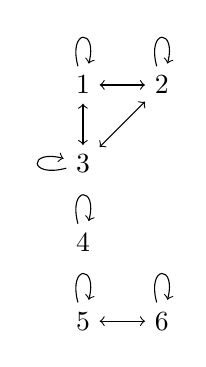
\begin{tikzpicture}
	\graph  {
		1 <-> 2;
		1 <-> 3;
		1 ->[loop above] 1;
		2 ->[loop above] 2;
		3 ->[loop left] 3;
		2 <-> 3;
		4 ->[loop above] 4;
		5 <-> 6;
		5 ->[loop above] 5;
		6 ->[loop above] 6;
		
	};
	
	
\end{tikzpicture}


\section{习题四 31}
\begin{solution}

\begin{itemize}
	\item[(1)]
	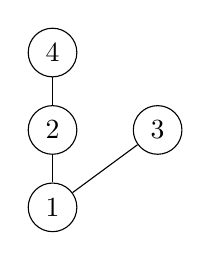
\begin{tikzpicture}[node distance=10pt]
		\node[draw, circle]                        (4)   {4};
		\node[draw, circle, below=of 4]                         (2)  {2};
		\node[draw, circle, right=20pt of 2]                        (3)  {3};
		\node[draw, circle, below=of 2]     (1)  {1};
		
		\graph{
			(4) -- (2) -- (1);
			(3) -- (1)
		};
	\end{tikzpicture}
	
	\item[(2)]
	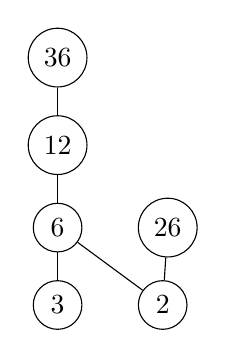
\begin{tikzpicture}[node distance=10pt]
		\node[draw, circle]                         (36)   {36};
		\node[draw, circle, below=of 36]             (12)  {12};
		\node[draw, circle, below=of 12]        (6)  {6};
		\node[draw, circle, below=of 6]     		(3)  {3};
		\node[draw, circle, right=20pt of 3]     		(2)  {2};
		\node[draw, circle, right=20pt of 6]     		(26)  {26};
		
		\graph{
			(36) -- (12) -- (6) -- (3);
			(6) -- (2);
			(26) -- (2);
		};
	\end{tikzpicture}
	
	\item[(3)]
	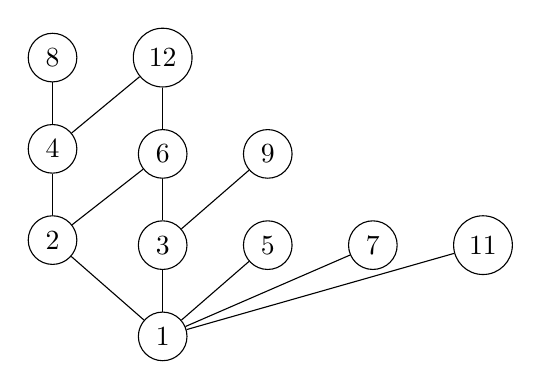
\begin{tikzpicture}[node distance=15pt]
		\node[draw, circle]                         (8)   {8};
		\node[draw, circle, right=20pt of 8]             (12)  {12};
		\node[draw, circle, below=of 12]        (6)  {6};
		\node[draw, circle, below=of 8]     		(4)  {4};
		\node[draw, circle, below=of 6]     		(3)  {3};
		\node[draw, circle, below=of 4]     		(2)  {2};
		\node[draw, circle, right=20pt of 3]             (5)  {5};
		\node[draw, circle, right=20pt of 5]             (7)  {7};
		\node[draw, circle, right=20pt of 7]             (11)  {11};
		\node[draw, circle, right=20pt of 6]             (9)  {9};
		\node[draw, circle, below=of 3]     		(1)  {1};
		
		\graph{
			(8) -- (4) -- (2) -- (1);
			(12) -- (6) -- (3) -- (1);
			(12) -- (4);
			(6) -- (2);
			(9) -- (3);
			(1) -- {
				(5),(7),(11)
			}
		};
	\end{tikzpicture}
	
	$\{2,3,6\}:6,\text{无},6,\{2,3\},6,1$.
	
	$\{2,4,6\}:\text{无},2,\{4,6\},2,\text{无},2$.
	
	$\{4,8,12\}:\text{无},4,\{8,12\},4,4,\text{无}$.
\end{itemize}
\end{solution}

\section{习题四 32}

\begin{solution}
	$A=\{0,1,2,3,4,5,6\}$.
	
	$\preceq=\{(0,0),(0,1),(0,2),(0,3),(0,4),(0,5),(0,6),(1,1),\\(2,2),(2,5),(3,3),(3,5),(5,5),(4,4),(4,6),(6,6)\}$.
\end{solution}

\section{习题四 34}

\begin{proof}
	自反: $\forall (a,b) \in A\times B$ 由 $(a,a) \in \preceq_1 \wedge (b,b) \in \preceq_2 \Rightarrow ((a,b),(a,b)) \in \preceq_3$.
	
	反对称: $\forall ((a_1,b_1),(a_2,b_2)) \in \preceq_3 \wedge ((a_2,b_2),(a_1,b_1)) \in \preceq_3, \\ (a_1,a_2),(a_2,a_1) \in \preceq_1 \wedge (b_1,b_2),(b_2,b_1) \in \preceq_2 \Rightarrow a_1=a_2\wedge b_1=b_2 \Rightarrow (a_1,b_1)=(a_2,b_2)$.
	
	传递: $\forall ((a_1,b_1),(a_2,b_2)),((a_2,b_2),(a_3,b_3)) \in \preceq_3, (a_1,a_2),(a_2,a_3) \in \preceq_1, \\ \Rightarrow (a_1,a_3)\in \preceq_1$ 同理 $(b_1,b_3) \in \preceq_2 \Rightarrow ((a_1,b_1),(a_3,b_3)) \in \preceq_3$.
	
	综上 $\preceq_3$ 是 $A\times B$ 上的半序关系.
\end{proof}

\section{习题四 37}

\begin{solution}
	\begin{itemize}
		\item[(1)] 半序
		\item[(2)] 良序
		\item[(3)] 良序
	\end{itemize}
\end{solution}
%\chapter{第四次作业}

\section{习题五 3}

\begin{itemize}[leftmargin=1.5cm]
	\item[(1)] 单射
	\item[(3)] 都不是
	\item[(5)] 双射
	\item[(7)] 都不是
\end{itemize}


\section{习题五 6}

\begin{proof}
	$f\subseteq g\Rightarrow \mathscr{D}(f)\subseteq\mathscr{D}(g)\Rightarrow\mathscr{D}(f)=\mathscr{D}(g)$.
	
	从而 $\forall x\in \mathscr{D}(g),f(x)=g(x),\Rightarrow g\subseteq f,\Rightarrow g=f.$
\end{proof}

\section{习题五 9}

\begin{solution}
	\begin{itemize}
		\item[(1)]
		$$
		\begin{array}{l}
			f\circ g=f(g(x))=f(x+2)=(x+2)^2-1=x^2+4x+3,\\
			g\circ f=g(f(x))=g(x^2-1)=x^2+1.
		\end{array}$$
		\item[(2)] $g$ 是双射, $f,f\circ g,g\circ f$ 均不是.
	\end{itemize}
\end{solution}

\section{习题五 10}

\begin{solution}
	\begin{itemize}
		\item[(1)] 取 $f=(1234)$ 即 $f(1)=2,f(2)=3,f(3)=4,f(4)=1$.
		$$
		\begin{array}{c}
			f^2=(13)(24) \\
			f^3=(4321) \\
			f^{-1}=f^3 \\
			f\circ f^{-1}=I_A
		\end{array}
		$$
		\item[(2)] 取 $g=(12)(34)$, 即 $g(1)=2,g(2)=1,g(3)=4,g(4)=3$.
	\end{itemize}
\end{solution}

\section{习题五 11}
\begin{solution}
	$
	P^{-1}=\left(\begin{array}{c}
		123 \\
		231
	\end{array}\right)
	,\quad
	P\circ P^{-1}=\left(\begin{array}{c}
		123 \\
		123
	\end{array}\right)
	$
\end{solution}
\section{习题五 12}
\begin{solution}
	\begin{itemize}
		\item[(1)] 不是, 因为 $A\cap B \subseteq B$.
		\item[(2)] 是, 因为 $A \subseteq B\cup A$.
		\item[(3)] 是, 因为 $A$ 无穷那么存在可数集 $C\subseteq A$, 又 $C\backslash B$ 仍为可数集且 $C\backslash B \subseteq A\backslash B$.
	\end{itemize}
\end{solution}

%\chapter{第五次作业}

\section{习题六 1}

\begin{solution}
\begin{itemize}
	\item[(1)] 是
	\item[(3)] 是
	\item[(5)] 不是
	\item[(7)] 是
	\item[(9)] 是
\end{itemize}
\end{solution}
\section{习题六 3}

\begin{solution}
\begin{itemize}
	\item[(1)] 设 $X=\{a,b\},a*b=a,a*a=a,b*b=a,b*a=b$.
	\item[(2)] 设 $X=\{a,b\},a*b=b,a*a=a,b*b=a,b*a=a$.
	\item[(3)] 对于左幺元, $e_l*e_r=e_r$, 对于右幺元 $e_l*e_r=e_l$, 故 $e_l=e_l*e_r=e_r$.
\end{itemize}
\end{solution}

\section{习题六 7}

\begin{solution}
	满足结合律: $x*y*k=x*k=x,x*(y*k)=x*y=x$.
	
	不满足交换律: $x*y=x,y*x=y$.
	
	没有幺元, 但有右幺元, 且每个元素都是右幺元.
	
	没有零元, 但有左零元, 且每个元素都是左零元.
	
	没有逆元.	
\end{solution}

\section{习题六 9}

\begin{proof}
	$\forall\ x\in S,\ x*x^2=x^2*x\Rightarrow x^=x$
\end{proof}

\section{习题六 12}

\begin{solution}
	$S_1,S_2$ 是, $S_3$ 不是.
\end{solution}

\section{习题六 17}

\begin{solution}
	取映射 $\varphi(x)=\left\{
	\begin{array}{l}
		0,\quad x=0\\
		1,\quad x\neq 0
	\end{array}
	\right.$
	
	则有 $\varphi(x)\varphi(y)=\varphi(xy)$.
	
	即 $\varphi$ 是同态.
\end{solution}

\section{习题六 19}

\begin{proof}
	$\forall\ a,b\in X,\ h(x)h(y)=f_1(x)\oplus f_2(x)\oplus f_1(y)\oplus f_2(y)=f_1(x)\oplus f_1(y)\oplus (f_2(x)\oplus f_2(y))=f_1(xy)\oplus f_2(xy)=h(xy)$.
\end{proof}

\section{习题六 22}

\begin{itemize}
	\item[(1)]
	
	$
	\begin{array}{c|cccccc}
		* & 0 & 1 & 2 & 3 & 4 & 5 \\\hline
		0 & 0 & 0 & 0 & 0 & 0 & 0 \\
		1 & 0 & 1 & 2 & 3 & 4 & 5 \\
		2 & 0 & 2 & 4 & 0 & 2 & 4 \\
		3 & 0 & 3 & 0 & 3 & 0 & 3 \\
		4 & 0 & 4 & 2 & 0 & 4 & 2 \\
		5 & 0 & 5 & 4 & 3 & 2 & 1 
	\end{array}
	$
	\item[(2)] $\forall\ x,y,z\in N_k$, 设 $x*y=p_1k+r_1,y*z=p_2k+r_2,x*y*k=p_3k+r_3$
	则有 $r_1z\equiv r_3(\bmod\ k),xr_2\equiv r_3(\bmod\ k),\Rightarrow x*_ky*_kz = r_1*_kz=r_3,x*_k(y*_kz)=x*_kr_2=r_3$.
	
	故满足结合律, 即 $<N_k,*_k>$ 是半群. 
	
\end{itemize}

\section{习题六 25}

\begin{proof}
	$\forall x,y,z\in \mathbb R,x*y*z=(x+y+xy)*z=x+y+xy+z+(x+y+xy)z=x+y+z+xy+xz+yz,\ x*(y*z)=x*(y+z+yz)=x+y+z+xy+xz+yz$.
	
	幺元是 $0$. $\forall x\in \mathbb R,0*x=0+x+0x=x,x*0=x+0+x0=x$.
	
	故 $<\mathbb R,*>$ 是半群.
\end{proof}

\section{习题六 30}
$<S,*>$ 是半群. 若有 $a\in S,\ \forall\ x\in S,\ \exists\ u,v\in S$ 使得 $$a*u=v*a=x$$ 证明: $<S,*>$ 是含幺半群.

\begin{proof}
先取 $x=a$, 设 $ab_1=b_2a=a$.

再取 $x=b_1$, 设 $b_1=au$ 同左乘 $b_2$ 得
$b_2b_1=b_2au=au=b_1$.

再取 $x=b_2$, 设 $b_2=va$ 同右乘 $b_1$ 得
$b_2b_1=vab_1=va=b_2$.

故得到 $b_1=b_2$ 记作 $b$, 即 $ab=ba=a$.

下面验证 $b$ 是幺元.

$\forall\ x\in S,$ 设 $x=au=va$ 则有 $bx=bau=au=x,xb=vab=va=x$.

故 $b$ 是幺元.
\end{proof}

\section{习题六 32}

\begin{itemize}
	\item[(1)]
	\begin{proof}
		$f_1,f_2\in S^S, \forall x\in S,f_1\circ f_2 (x)=f_1(f_2(x))$ 由 $f_2(x)\in S\Rightarrow f_1(f_2(x))\in S\Rightarrow f_1\circ f_2\in S^S$.
		
		又函数的复合具有结合律, $<S^S,\circ>$ 是半群. 
	\end{proof}
	\item[(2)]
	\begin{solution}
		对于给定 $a$ 设 $\sigma_a: S\to S,\sigma_a(x)=ax$.
		
		则有 $\sigma_a\in S^S$.
		
		取 $\varphi:S\to S^S,\varphi(a)=\sigma_a$.
		
		$\forall\ a,b\in S,\forall x\in S,\varphi(a)\circ\varphi(b)(x)=\sigma_a(\sigma_b(x))=abx=\sigma_{ab}x=\varphi(ab)(x)$ 即 $\varphi$ 是同态.
	\end{solution}
\end{itemize}

\section{习题六 33}

\begin{proof}
	设 $y=f(x)\in Y$ 则 $y*y=f(x)*f(x)=f(x^2)=f(x)=y$ 故 $y$ 是 $Y$ 的幂等元.
\end{proof}

\section{习题六 34}

\begin{itemize}
	\item[(1)] 真
	\item[(2)] 真
	\item[(2)] 真
\end{itemize}

\section{习题六 43}

$x*x=e$ 即 $S$ 中的元素均存在逆元. 故 $<S,*>$ 是群.

$yx=yx*e=yx*y^2=yx*y*e*y=yx*y*x^2*y=(yx)^2xy=e*xy=xy$.

故 $<S,*>$ 是交换群.

\section{习题六 47}

\begin{proof}
	先证必要性, $H_1H_2$ 是 $G$ 的子群, $\forall h_1h_2\in H_1H_2,(h_1h_2)^{-1}\in H_1H_2,\Rightarrow\exists h_1'h_2'=(h_1h_2)^{-1},\Rightarrow h_1h_2=(h_1'h_2')^{-1}=h_2'^{-1}h_1'^{-1}\in H_2H_1\Rightarrow H_1H_2\subseteq H_2H_1$.
	
	又 $\forall\ h_2h_1\in H_2H_1,h_1^{-1}h_2^{-1}\in H_1H_2\Rightarrow (h_1^{-1}h_2^{-1})^{-1}\in H_1H_2\Rightarrow h_2h_1\in H_1H_2\Rightarrow H_2H_1\subseteq H_1H_2$.
	
	综上 $H_1H_2=H_2H_1$. 
	
	下证充分性, $\forall h_1h_2,h_3h_4\in H_1H_2$ 对于 $(h_3h_4)^{-1}=h_4^{-1}h_3^{-1}$ 存在 $h_3'h_4'=(h_3h_4)^{-1},h_3'\in H_1,h_4'\in H_2$.
	
	则 $h_1h_2(h_3h_4)^{-1}=h_1h_2h_3'h_4'$, 对于 $h_2h_3$ 存在 $h_3''\in H_1,h_2''\in H_2,h_2h_3=h_3''h_2''$.
	
	即 $h_1h_2h_3'h_4'=(h_1h_3'')(h_2''h_4'),h_1h_3''\in H_1,h_2''h_4\in H_2\Rightarrow h_1h_2(h_3h_4)^{-1}\in H_1H_2$ 故 $H_1H_2$ 是 $G$ 的子群.
\end{proof}

\section{习题六 49}

\begin{proof}
	$\forall\ x,y\in X,\ yH=Hy\Rightarrow H=y^{-1}Hy\Rightarrow Hy^{-1}=y^{-1}H\Rightarrow y^{-1}\in X$, 
	又 $xy^{-1}H=x(y^{-1}H)=x(Hy^{-1})=(xH)y^{-1}=H(xy^{-1})\Rightarrow xy^{-1}\in X$
	
	故 $X$ 是 $G$ 的子群.
\end{proof}

\section{习题六 50}

\begin{itemize}
	\item[(1)]
	\begin{proof}
		封闭性: $f_1=a_1x+b_1,f_2=a_2x+b_2\Rightarrow f_1\circ f_2=f_1(a_2x+b_2)=a_1a_2x+a_1b_2+b_1\in G$.
		
		函数的复合满足结合律.
		
		逆元: $f=ax+b,f^{-1}=\dfrac{x}{a}-\dfrac b a$.
		
		幺元: $f_e=x$.
		
		所以 $<G,\circ>$ 是群.
	\end{proof}
	\item[(2)]
	\begin{proof}
		$f_1,f_2\in S_1$ 设 $f_1=x+b_1,f_2=x+b_2,f_2^{-1}=x-b_2$, 则 $f_1\circ f_2^{-1}=x+b_1-b_2\in S_1$.
		
		$f_1,f_2\in S_2$ 设 $f_1=a_1x,f_2=a_2x,f_2^{-1}=\dfrac{x}{a_2}$, 则 $f_1\circ f_2^{-1}=\dfrac{a_1x}{a_2}\in S_2$.
		
		故 $<S_1,\circ>,<S_2,\circ>$ 是 $G$ 的子群.
	\end{proof}
\end{itemize}
\chapter*{第六次作业}

\problem[习题六 54]

\begin{proof}
	设 $G$ 的生成元为 $a$, 同态为 $\sigma$, 那么 $\forall b\in \sigma(G),\ \exists a^m\in G,\ s.t. \sigma(a^m)=b$. 从而 $b=\sigma(a^m)=\sigma(a)^m$. 即 $\sigma(G)$ 中的所有元素都可以表示成 $\sigma(a)$ 的整数次幂, 进而 $\sigma(G)=\langle \sigma(a)\rangle$ 是循环群.
\end{proof}

\problem[习题六 56]

\begin{proof}
	$\forall\ a,b\in H,f(a)=g(a),f(b)=g(b),f(ab^{-1})=f(a)+f(b^{-1})=f(a)-f(b)=g(a)-g(b)=g(a)+g(b^{-1})=g(ab^{-1})\Rightarrow ab^{-1}\in H$ 从而说明 $H<X$.
\end{proof}

\problem[习题六 57]

\begin{proof}
	\begin{itemize}
		\item[(1)] 自反性:
			$x=x*x*x^{-1}\Rightarrow (x,x)\in R$.
		\item[(2)] 对称性:
			若 $(x,y)\in R,\ \exists z\in G,\ s.t. y=z*x*z^{-1}\Rightarrow x=z^{-1}*y*(z^{-1})^{-1})\Rightarrow (y,x)\in R$.
		\item[(3)] 传递性:
			若 $(a,b),(b,c)\in R,\ \exists d,e\in G,\ s.t. b=d*a*d^{-1},c=e*b*e^{-1}\Rightarrow c=e*d*a*d^{-1}*e^{-1}=(e*d)*a*(e*d)^{-1}\Rightarrow (a,c)\in R$.
	\end{itemize}
	综上, $R$ 是等价关系.
\end{proof}

\problem[习题六 58]

\begin{proof}
	\begin{itemize}
		\item[(1)] $\forall a\in G$ 若 $a\in H$, 则有 $aH=H=Ha$, 若 $a\notin H$, 则取陪集分解 $G=H\cup aH=H\cup Ha$, 从而 $aH=Ha$.

		所以 $H\lhd G$.
		\item[(2)] $\forall a\in G$, 由于 $H$ 中元素和 $a$ 可交换从而直接有 $aH=Ha$.
		\item[(3)] $\forall a\in G$, $a(H_1\cap H_2)=aH_1\cap aH_2=H_1a\cap H_2a(H_1\cap H_2)a$.
	\end{itemize}
\end{proof}

\problem[习题六 59]

\begin{proof}
	零元: $1$

	幺元: $0$

	显然在整数中封闭并满足交换律.
\end{proof}

\problem[习题六 60(1,3,5)]

\begin{itemize}
	\item[(1)]不是, 没有幺元.
	\item[(3)]是.
	\item[(5)]是.
\end{itemize}

\problem[习题六 62]

\begin{solution}
	是环, 有零因子, $(x,0),(0,y),x,y\in \Q$.

	幺元 $(1,1)$.

	$(x,y),\ xy\neq 0$ 有逆元.
\end{solution}

\problem[习题六 65]

\begin{solution}
	\begin{itemize}
		\item[(1)]\

		\begin{itemize}
			\item[m=6]\

			子环: $\{0\},\{0,1,2,3,4,5\},\{0,2,4\},\{0,3\}$

			理想: $\{0\},\{0,1,2,3,4,5\},\{0,2,4\},\{0,3\}$
			\item[m=8]\

			子环: $\{0\},\{0,1,2,3,4,5,6,7\},\{0,2,4,6\},\{0,4\}$

			理想: $\{0\},\{0,1,2,3,4,5,6,7\},\{0,2,4,6\},\{0,4\}$
			\item[m=11]\

			子环: $\{0\},\{0,1,2,3,4,5,6,7,8.9,10\}$

			理想: $\{0\},\{0,1,2,3,4,5,6,7,8,9,10\}$
		\end{itemize}
		\item[(2)]
	\end{itemize}
\end{solution}

\problem[习题六 68(2)(4)]

是.

\problem[习题六 69]



		%\inmainbodyfalse
\part{数据结构与算法综合训练}
\chaptermark{数据结构与算法综合训练}
\inmainbodytrue
\chapter{实验 1: 渐进分析和排序算法}
%\addcontentsline{toc}{chapter}{实验 1: 渐进分析和排序算法}
\section{Task 1}

\begin{itemize}
	\item[(1)] 使用 $\t O,\Omega$ 和 $\Theta$ 的定义, 证明下面每一个等式:
	\begin{itemize}
		\item[a)] $2\sqrt n + 6 = \t O(\sqrt n)$
		\begin{proof}
			取 $C=8$ 则, $2\sqrt n + 6 \leq 8\sqrt n$ 故 $2\sqrt n + 6 = \t O(\sqrt n)$
		\end{proof}
		\item[b)] $n^2=\Omega(n)$
		\begin{proof}
			取 $C=1$ 则, $n^2\geq n$ 故 $n^2=\Omega(n)$.
		\end{proof}
		\item[c)] $\log_2(n)=\Theta(\ln (n))$
		\begin{proof}
			取 $C=\log_2 e$ 则, $\frac 1 C \log_2 (n)=\ln (n)$
			故 $\log_2 (n)=\Theta(\ln (n))$.
		\end{proof}
		\item[d)] $4^n\neq \t O(2^n)$
		\begin{proof}
			$\forall C>0,\ \exists n=\lceil \log_2 C\rceil \ s.t. 4^n\geq 2^n$ 故 $4^n\neq \t O(2^n)$
		\end{proof}
	\end{itemize}
	\item[(2)] 使用数学归纳法证明 $T(n)=\t O(n^2)$. 其中
	
	$
	T(n)=\left\{
	\begin{aligned}
		T(n-1)+2n, & n>1 \\
		3, & n=1
	\end{aligned}
	\right.
	$
	\begin{proof}
		$n=1$ 时, 取 $C=3$ 则, $T(1)=\t O(1)$.
		
		设 $n=k$ 时成立, 即 $T(k)=\t O(k^2)$
		
		则存在 $C>0$ 使得 $T(k)\le Ck^2$
		
		当 $n=k+1$ 时.
		
		$T(k+1)=T(k)+2(k+1) \le Ck^2+2k+2 = (C-1)k^2+(k+1)^2 + 1 \le C(k+1)^2$ 当 $C=3$ 时.
		
		综上 $T(n)=\t O(n^2)$.
	\end{proof}
\end{itemize}

\section{Task 2}

\subsection{算法设计}

先将所有点按照 $x_i$ 为第一关键字, $y_i$ 为第二关键字排序, 并以点 $p_m(m=\lfloor\frac n 2\rfloor)$ 为分界点, 拆分点集 $A_1,A_2$:

$A_1=\{p_i|i=0\ldots m\} \qquad A_2=\{p_i|i=m+1\ldots n-1\}$

并递归下去, 求出两点集各自内部的最近点对, 设距离为 $h_1,h_2$, 取较小值设为 $h$.

我们将所有横坐标与 $x_m$ 的差小于 $h$ 的点放入集合 $B=\{p_i| |x_i-x_m|<h \}$ 而只有这些点内部的点距离可能更优. 

同样的, 如果想比 $h$ 更小, $B$ 中点的纵坐标之差也得小于 $h$.

我们设 $C(p)=\{p_i|p_j\in B,y_i-h<y_j\le y_i\}$.

接下来只需对每对 $p_i\in B,p_j\in C(p_i)$ 求距离并取最小值即可.

至此我们已经完成了这个问题, 但还有一些实现的细节需要完善, 比如如何快速计算 $C$ 数组. 这将在复杂度分析中给出具体方式及其正确性证明.

\subsection{复杂度分析}

我们先来考虑 $C$ 的计算方式, 最朴素的想法就是将 $B$ 中的点按 $y_i$ 排序, 就可以得到.

但是如果每次直接排序, 这部分的复杂度就变为 $\t O(n\log ^2 n)$. 超出了预期.

但仔细思考后, 在求 $B$ 的时候我们已经不需要 $x_i$ 的顺序了, 所以在递归过程中我们可以利用归并排序对 $y$ 进行排序, 由此我们就可以在 $\t O(n\log n)$ 的时间复杂度内求出 $C$.

除此之外, 在每次求完 $C$ 并更新答案时我们的复杂度为 $|C|$, 而粗略看去 $|C|$ 应该是 $\t O(n)$ 级别, 那么总复杂度将退化为 $\t O(n^2)$. 但经过仔细分析后实则不然, $C$ 的大小并没有那么大, 最大大小实际上只有 $7$. 我们进一步考虑 $C$ 的定义, 发现 $C(p_i)$ 内部的点应该落在 $(x_m-h,x_m+h) \times (y_i-h,y_i]$ 这个大小为 $2h\times h$ 的矩形内, 而当我们以中心线 $x_m$ 将其分成两个部分. 

下面只考虑左半部分, 由于左半边被之前分治的左半边包含, 所以该区域内任意两点的距离应该不小于 $h$, 而该部分的面积为 $h\times h$. 更进一步的, 我们将这个 $h\times h$ 的矩形分成四个 $\frac h 2 \times \frac h 2$ 的小矩形, 则每个小矩形内部最多只会存在一个点, 因为小矩形的对角线长度也仅有 $\frac {h} {\sqrt 2}<h$ 所以在整个 $2h\times h$ 中最多只会存在 $8$ 个点, 再除去 $p_i$ 本身, 就只会剩下 $7$ 个点.

通过上述分析, 我们分治之后合并的复杂度是 $\t O(n)$.

那么总复杂度就是 $T(n)=2T(\frac n 2)+\t O(n)=\t O(n\log n)$.

\subsection{代码实现}

代码如下, 已通过洛谷 P7883 平面最近点对(加强加强版)

\begin{lstlisting}
const int N=4e5+10;
const ll INF=9e18;
int n;
struct Point{
	int x,y;
}a[N],b[N];
bool cmp(Point a,Point b)
{
	return a.x<b.x;
}
bool cmp2(Point a,Point b)
{
	return a.y<b.y;
}
ll dist(Point a,Point b)
{
	return 1ll*(a.x-b.x)*(a.x-b.x)+1ll*(a.y-b.y)*(a.y-b.y);
}
ll solve(int l,int r)
{
	if(r-l<=10)
	{
		ll ans=INF;
		sort(a+l,a+r+1,cmp2);
		for(int i=l;i<=r;i++)
		for(int j=i+1;j<=r;j++)
		ans=min(ans,dist(a[i],a[j]));
		return ans;
	}
	int mid=(l+r)>>1;
	int px=a[mid].x;
	ll ans=INF;
	ans=min(solve(l,mid),solve(mid+1,r));
	int p1=l,p2=mid+1,p3=l;
	while(p1<=mid&&p2<=r)
	{
		if(a[p1].y<a[p2].y)b[p3++]=a[p1++];
		else b[p3++]=a[p2++];
	}
	while(p1<=mid)b[p3++]=a[p1++];
	while(p2<=r)b[p3++]=a[p2++];
	for(int i=l;i<=r;i++)a[i]=b[i];
	int tot=0;
	for(int i=l;i<=r;i++)
	if(1ll*abs(a[i].x-px)*abs(a[i].x-px)<ans)
	{
		for(int j=tot;j&&1ll*(a[i].y-b[j].y)*(a[i].y-b[j].y)<ans;--j)
		ans=min(ans,dist(a[i],b[j]));
		b[++tot]=a[i];
	}
	return ans;
}
int main()
{
	read(n);
	for(int i=1;i<=n;i++)
	read(a[i].x),read(a[i].y);
	sort(a+1,a+n+1,cmp);
	cout<<solve(1,n);
	return 0;
}
\end{lstlisting}

\section{Task 3}

以下为各排序算法的主干代码. 均用 $50$ 组不同规模随机数据, 正序数据和逆序数据进行测试.

\subsection{插入排序}

\begin{lstlisting}
void Insertion(vector<int>&num)
{
	int n=num.size();
	for(int i=1;i<n;i++)
	{
		int pos=i;
		for(int j=i-1;j>=0;j--)
		if(num[i]<num[j])
			pos=j;
		int val=num[i];
		for(int j=i;j>pos;j--)num[j]=num[j-1];
		num[pos]=val;
	}
	return;
}
\end{lstlisting}

\subsection{选择排序}

\begin{lstlisting}
void Selection(vector<int>&num)
{
	int n=num.size();
	for(int i=0;i<n-1;i++)
	{
		int pos=i;
		for(int j=i;j<n;j++)
		if(num[j]<num[pos])pos=j;
		swap(num[i],num[pos]);
	}
	return;
}
\end{lstlisting}

\subsection{希尔排序}

\begin{lstlisting}
void Shell_1(vector<int>&num)
{
	static int H[30];
	int n=num.size(),p=0;
	H[p]=1;
	for(;H[p]<n;p++)
	H[p+1]=H[p]<<1;
	while (p>=0)
	{
		int h=H[p];
		for (int i = h; i < n; i++)
		for (int j = i; j >= h && num[j] < num[j - h]; j -= h)
		swap(num[j], num[j - h]);
		p--;
	}
	return;
}
\end{lstlisting}

其余两个希尔排序只有 $H$ 数组发生变化, 变化如下:

\begin{lstlisting}
for(;H[p]<n;p++)
	H[p+1]=((H[p]+1)<<1)-1;
\end{lstlisting}

\begin{lstlisting}
for(;H[p]<n;p++)
	H[p+1]=((H[p]<<1|1)*3-1)/2;
\end{lstlisting}

\subsection{快速排序}

\begin{lstlisting}
int depth=0;
void Quicksort(vector<int>&num,int l,int r,int dep)
{
	depth=max(depth,dep);
	if(l==r)return;
	int pos=random(l,r); //在 [l,r] 中随机选取点, 利用 c++ rand() 函数实现
	int p=num[pos];
	swap(num[pos],num[r]);
	int i=l,j=r-1;
	while(i<j)
	{
		while(i<j&&num[i]<p)i++;
		while(i<j&&num[j]>=p)j--;
		swap(num[i],num[j]);
	}
	if(num[i]>=num[r])swap(num[i],num[r]);
	else i++;
	if(l<i)Quicksort(num,l,i-1,dep+1);
	if(i+1<=r)Quicksort(num,i+1,r,dep+1);
	return;
}
\end{lstlisting}

\subsection{归并排序}

\begin{lstlisting}
void Mergesort(vector<int>&num,int l,int r)
{
	static vector<int>tmp;
	if(l==r)return;
	int mid=(l+r)>>1;
	Mergesort(num,l,mid);
	Mergesort(num,mid+1,r);
	if(tmp.size()<r-l+1)tmp.resize(r-l+1);
	int p1=l,p2=mid+1,p=0;
	while(p1<=mid&&p2<=r)
	{
		if(num[p1]<num[p2])tmp[p++]=num[p1++];
		else tmp[p++]=num[p2++];
	}
	while(p1<=mid)tmp[p++]=num[p1++];
	while(p2<=r)tmp[p++]=num[p2++];
	for(int i=l;i<=r;i++)num[i]=tmp[i-l];
}
\end{lstlisting}

\section{Task 4}

以下为各排序算法实际运行时间测试, 同一组数据采取运行 $20$ 次所需时间的平均值.

考虑到选择和插入排序的效率过慢, 故对其余算法进行了更大数据集的测试和单独的图表绘制. 以此更清晰的表示其余算法的效率差异.

\subsection{随机数据}

\begin{figure}[H]    % 常规操作\begin{figure}开头说明插入图片
	% 后面跟着的[htbp]是图片在文档中放置的位置,也称为浮动体的位置,关于这个我们后面的文章会聊聊,现在不管,照写就是了
	\centering            % 前面说过,图片放置在中间
	\subfloat[所有算法]   % 第一张子图的下标(注意:注释要写在[]中括号内)
	{
		\label{fig:subfig1}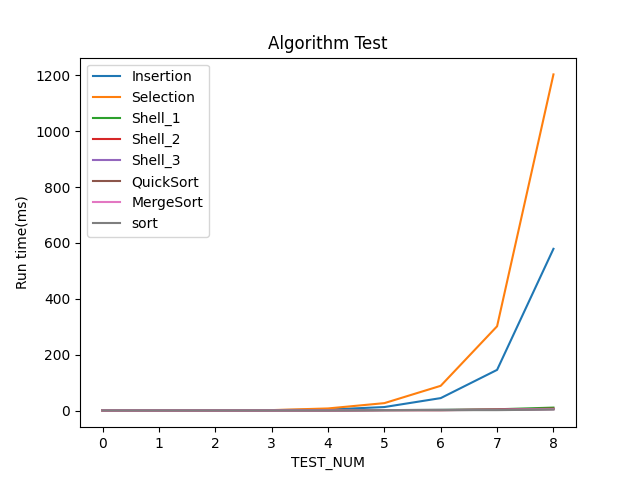
\includegraphics[width=0.4\textwidth]{figures/1_1.png}
	}
	\subfloat[去除插入和选择]
	{
		\label{fig:subfig2}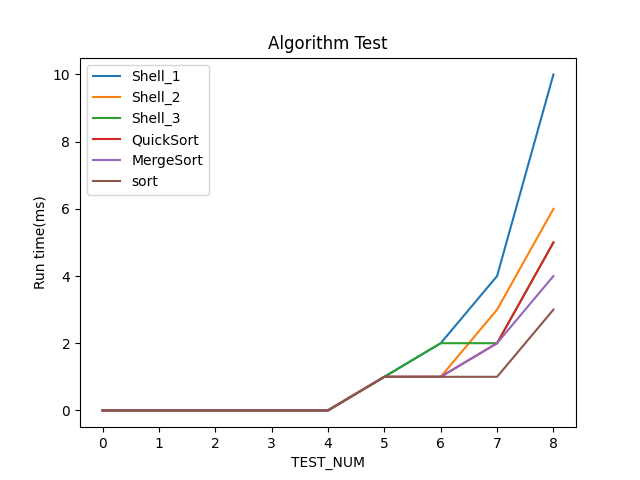
\includegraphics[width=0.4\textwidth]{figures/1_2.png}
	}
	\\
	\subfloat[更大测试数据]   % 第一张子图的下标(注意:注释要写在[]中括号内)
	{
		\label{fig:subfig3}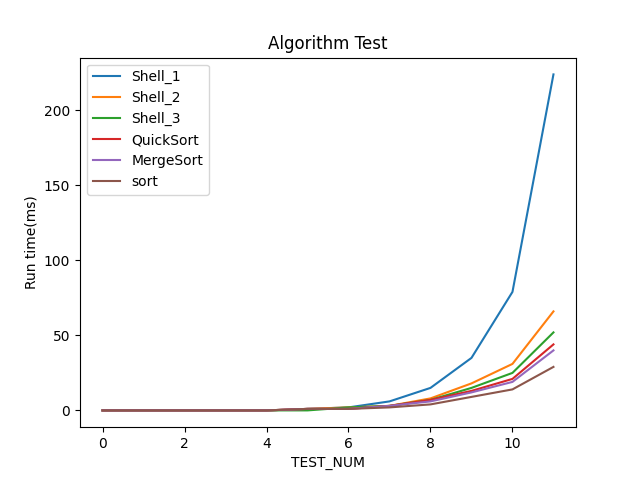
\includegraphics[width=0.4\textwidth]{figures/1_3.png}
	}
	\subfloat[更大测试数据并去除 Shell\_1]
	{
		\label{fig:subfig4}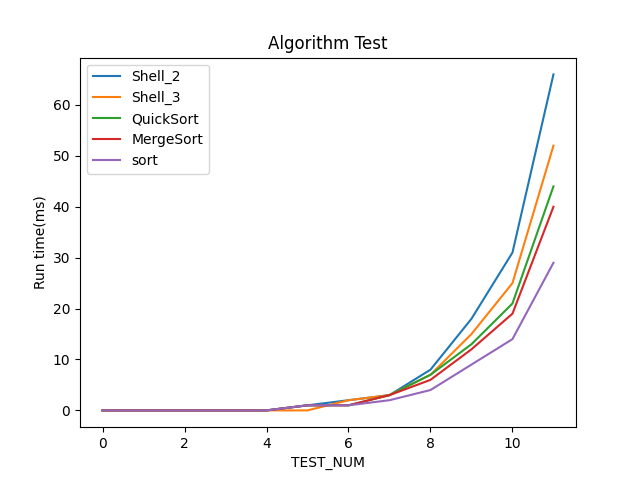
\includegraphics[width=0.4\textwidth]{figures/1_4.png}
	}
	\caption{随机数据}    % 整个图片的说明,注释写在{}内
	\label{fig:subfig_1}   
\end{figure}

\subsection{正序数据}

\begin{figure}[H]    % 常规操作\begin{figure}开头说明插入图片
		% 后面跟着的[htbp]是图片在文档中放置的位置,也称为浮动体的位置,关于这个我们后面的文章会聊聊,现在不管,照写就是了
		\centering            % 前面说过,图片放置在中间
		\subfloat[所有算法]   % 第一张子图的下标(注意:注释要写在[]中括号内)
		{
			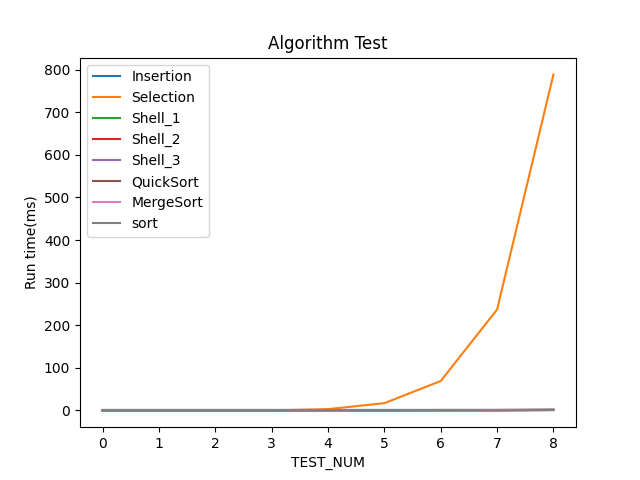
\includegraphics[width=0.4\textwidth]{figures/2_1.png}
		}
		\subfloat[去除插入和选择]
		{
			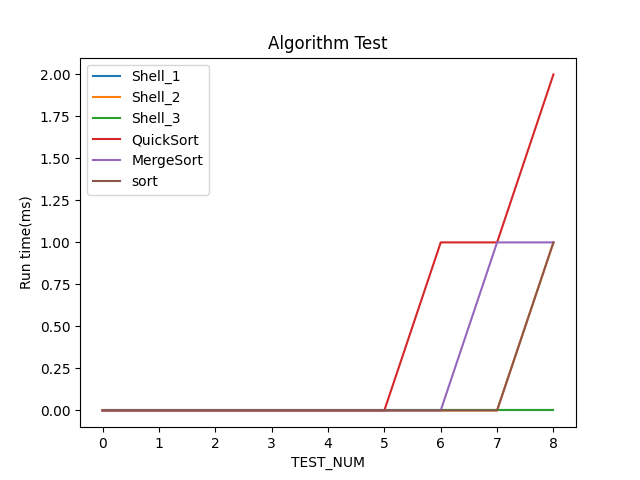
\includegraphics[width=0.4\textwidth]{figures/2_2.png}
		}
		\caption{正序数据}    % 整个图片的说明,注释写在{}内
		
\end{figure}

\subsection{逆序数据}

\begin{figure}[H]    % 常规操作\begin{figure}开头说明插入图片
		% 后面跟着的[htbp]是图片在文档中放置的位置,也称为浮动体的位置,关于这个我们后面的文章会聊聊,现在不管,照写就是了
		\centering            % 前面说过,图片放置在中间
		\subfloat[所有算法]   % 第一张子图的下标(注意:注释要写在[]中括号内)
		{
			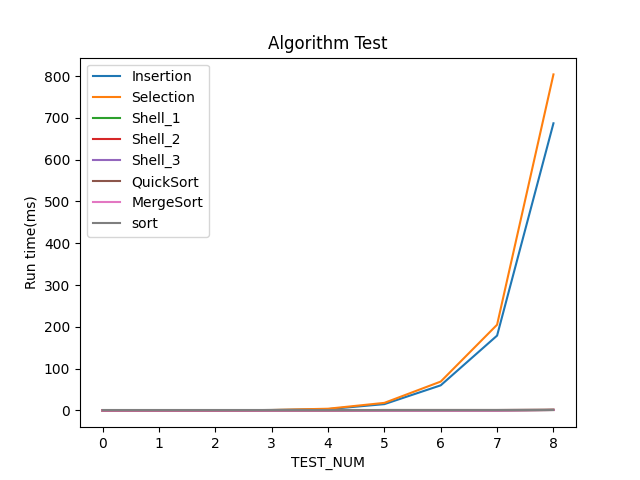
\includegraphics[width=0.4\textwidth]{figures/3_1.png}
		}
		\subfloat[去除插入和选择]
		{
			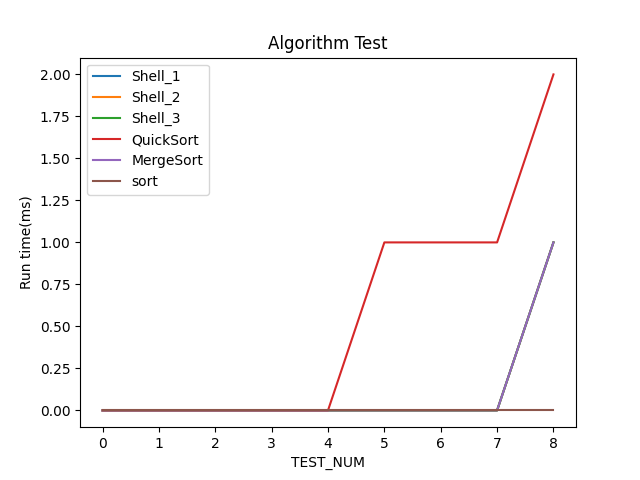
\includegraphics[width=0.4\textwidth]{figures/3_2.png}
		}
		\caption{逆序数据}    % 整个图片的说明,注释写在{}内
		
\end{figure}

\subsection{总结}

从理论分析上看, 插入排序和选择排序的时间复杂度均为 $\t O(n^2)$ 级别, 而快排和归并排序均为 $\t O(n\log n)$, 而实际测试中, 这两种算法的实际用时也确实远超过其余算法.

而对于希尔, 快排, 归并和 C++ stl 中的 sort 函数. Shell\_1 在小数据与其他算法时间差距不大, 但当数据规模进一步扩大后, 用时增长速度明显大于其余算法. 而 Shell\_2 在大数据规模下也有较差的表现.

而快排和归并, 则一直用时接近, 只有细微差别. C++ stl 中的 sort 函数表现出了较优的性能.

对于不同的数据性质选择, 快排, 归并和希尔用时变化不大. 

而插入排序, 如果是从后往前寻找插入位置时, 当数据为正序理论复杂度为 $\t O(n)$, 实际运行效率也很高.

\section{Task 5}

\subsection{快排层数}

\begin{figure}[H]
	\centering
	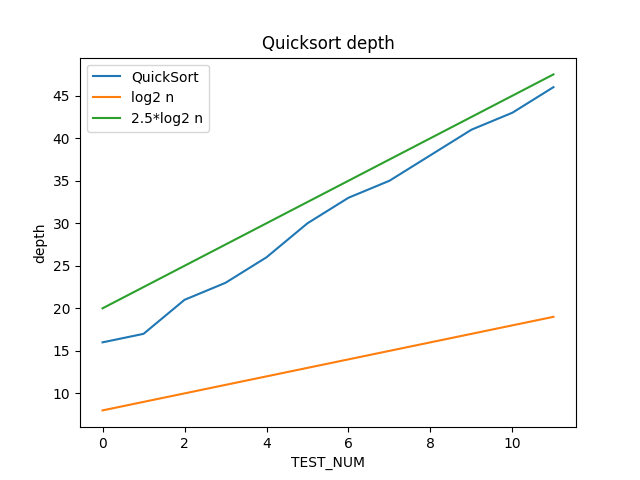
\includegraphics[width=0.8\textwidth]{figures/quick_dep.png}
\end{figure}

在 $2^8\sim 2^{19}$ 这 12 组数据测试结果中, 从图中可以看出递归深度大概是一个 $\t O(\log_2 n)$ 级别.

而从理论分析上看, 快排轴值的选取期望就是中间值, 故理论上递归层数就应该是 $\t O(\log_2 n)$ 级别.

\subsection{快排优化}

\begin{figure}[H]
	\centering
	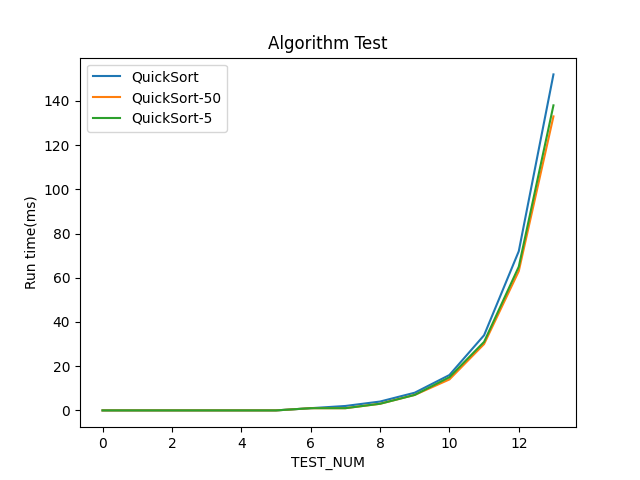
\includegraphics[width=0.8\textwidth]{figures/quick.png}
\end{figure}

通过设定阈值分别为 $50$ 和 $5$, 在 $2^8\sim 2^{21}$ 这些数据中, 可以看出, 优化过的两份算法均略优于没优化过的快排.
但优化幅度并不大, 只是常数上的优化, 并不影响算法复杂度.

而对于不同的阈值, 由此实验看出 $50$ 比 $5$ 快了几毫秒, 基本区别不大.

\subsection{螺丝螺母匹配问题}:
 
由于我们无法直接比较螺丝或螺母的大小, 所以考虑先找到一个轴值, 并利用轴值与相对的类别进行比较.

具体的, 类似快排, 我们先选取一个轴值螺母, 将这个螺母与区间内每个螺丝比较, 找到与该轴值螺母匹配的螺丝, 记为轴值螺丝.

接下来利用轴值螺母对所有螺丝做快排的操作, 利用轴值螺丝对所有螺母做快排的操作.

之后只需类似快排的递归调用即可.

程序实现:

 \begin{lstlisting}
 int match(int nut,int bolt)
 {
 	return nut==bolt?0:nut>bolt?1:-1;
 }
 void Quicksort(vector<int>&nuts,vector<int>&bolts,int l,int r)
 {
 	if(l==r)return;
 	int pos_nut=random(l,r);
 	int p_nut=nuts[pos];
 	int pos_bolt=l,p_bolt;
 	for(int i=l;i<=r;i++)
 	if(match(p_nut,bolts[i])==0)pos_bolt=i;
 	p_bolt=bolts[pos_bolt];
 	swap(nut[pos_nut],nut[r]);
 	swap(bolt[pos_bolt],bolt[r]);
 	int i=l,j=r-1;
 	while(i<j)
 	{
 		while(i<j&&match(nut[i],p_bolt)==-1)i++;
 		while(i<j&&match(nut[j],p_blot)>=0)j--;
 		swap(num[i],num[j]);
 	}
 	if(match(nut[i],p_bolt)==1)swap(nut[i],nut[r]);
 	else i++;
 	
 	i=l,j=r-1;
 	while(i<j)
 	{
 		while(i<j&&match(p_nut,bolt[i])==1)i++;
 		while(i<j&&match(p_nut,bolt[i])<=0)j--;
 		swap(num[i],num[j]);
 	}
 	
 	if(match(p_nut,bolts[i])==-1)swap(bolts[i],bolts[r]);
 	else i++;
 	if(l<i)Quicksort(nuts,bolts,l,i-1);
 	if(i+1<=r)Quicksort(nuts,bolts,i+1,r);
 	return;
 }
 \end{lstlisting}

\chapter{实验 2: 线性表实现及应用}
%\addcontentsline{toc}{chapter}{实验 1: 渐进分析和排序算法}
\section{Task 1: 为指定的 List ADT 实现各种数据结构}

\subsection{代码实现}

\subsubsection{顺序数组}

\begin{lstlisting}
template<typename T>
class List_ADT{
	int cursor, len;
	vector<T> val;
	public:
	void init(int length)
	{
		val.resize(length);
		cursor = -1;
		len = 0;
		return;
	}
	
	void insert(T newElement)
	{
		if(isFull())
		{
			printf("Error! Out of the list capacity!\n");
			return;
		}
		for(int i = len;i > cursor + 1; i--)
		val[i] = val[i - 1];
		len ++;
		val[++ cursor] = newElement;
	}
	void remove()
	{
		if(isEmpty()) return;
		len --;
		for(int i = cursor; i < len; i ++)
		val[i] = val[i + 1];
		cursor = cursor == len ? 0 : cursor;
		if(len == 0)
		cursor = -1;
		return;
	}
	void replace(T newElement)
	{
		if(isEmpty()) return;
		val[cursor] =  newElement;
		return;
	}
	void clear()
	{
		len = 0;
		cursor = -1;
		return;
	}
	bool isEmpty()
	{
		return len == 0;
	}
	bool isFull()
	{
		return len == (int)val.size();
	}
	bool gotoBeginning()
	{
		if(isEmpty()) return false;
		else
		{
			cursor = 0;
			return true;
		}
	}
	bool gotoEnd()
	{
		if(isEmpty()) return false;
		else
		{
			cursor = len - 1;
			return true;
		}
	}
	bool gotoNext()
	{
		if(cursor + 1 != len)
		{
			cursor ++;
			return true;
		}
		else return false;
	}
	bool gotoPrev()
	{
		if(isEmpty()) return false;
		else if(cursor == 0) return false;
		else
		{
			cursor --;
			return true;
		}
	}
	T getCursor()
	{
		if(isEmpty()) return 0;
		return val[cursor];
	}
	void showStructure()
	{
		if(isEmpty()) printf("Empty list ");
		else
		{
			for(int i=0;i<len;i++) 
			putchar(val[i]),putchar(' ');
		}
		printf("{capacity = %d, length = %d, cursor = %d}\n",(int)val.size(),len,cursor);
	}
	void moveToNth(int n)
	{
		T tmp = getCursor();
		remove();
		cursor = n - 1;
		insert(tmp);
	}
	bool find(T searchElement)
	{
		while(getCursor() != searchElement&&gotoNext());
		return getCursor() == searchElement;
	}
};
char s[100010];
int main()
{
	freopen("list_testcase.txt","r",stdin);
	freopen("数组.txt","w",stdout);
	List_ADT<char> a;
	a.init(512);
	while(gets(s) != NULL)
	{
		int n = strlen(s);
		for(int i = 0; i < n; i ++)
		{
			if(s[i] == ' ')	continue;
			if(s[i] == '+')
				a.insert(s[++i]);
			else if(s[i] == '-')
				a.remove();
			else if(s[i] == '=')
				a.replace(s[++ i]);
			else if(s[i] == '#')
				a.gotoBeginning();
			else if(s[i] == '*')
				a.gotoEnd();
			else if(s[i] == '>')
				a.gotoNext();
			else if(s[i] == '<')
				a.gotoPrev();
			else if(s[i] == '~')
				a.clear();
		}
		a.showStructure();
	}
	return 0;
}

\end{lstlisting}

\subsubsection{单向链表}

主函数同上, 此处不多赘述.

\begin{lstlisting}
template<typename T>
class List_ADT{
	int cursor, len, lenLimit;
	struct Point{
		T val;
		Point *next;
	};
	Point *head = nullptr, *p = nullptr, *tmp = nullptr;
	public:
	void init(int length)
	{
		head = nullptr;
		cursor = -1;
		len = 0;
		lenLimit = length;
		return;
	}
	
	void insert(T newElement)
	{
		if(isFull())
		{
			printf("Error! Out of the list capacity!\n");
			return;
		}
		if(len == 0)
		{
			head = p = new Point;
			p -> next = nullptr;
			p -> val = newElement;
		}
		else
		{
			tmp = p -> next;
			p -> next = new Point;
			p = p -> next;
			p -> val = newElement;
			p -> next = tmp;
		}
		len ++;
		cursor ++;
		return;
	}
	
	void remove()
	{
		if(isEmpty()) return;
		if(p == head)
		{
			p = head -> next;
			free(head);
			head = p;
		}
		else
		{
			tmp = p;
			gotoPrev();
			p -> next = tmp -> next;
			free(tmp);
			p = p -> next;
			cursor ++;
			if(p == nullptr) p = head, cursor = 0;
		}
		len --;
		if(len == 0)
		{
			cursor = -1;
			head = p = nullptr;
		}
		return;
	}
	void replace(T newElement)
	{
		if(isEmpty()) return;
		p->val = newElement;
		return;
	}
	void clear()
	{
		len = 0;
		cursor = -1;
		p = head;
		while(p!= nullptr)
		{
			tmp = p;
			p = p -> next;
			free(tmp);
		}
		head = p = nullptr;
		return;
	}
	
	bool isEmpty()
	{
		return len == 0;
	}
	
	bool isFull()
	{
		return len == lenLimit;
	}
	
	bool gotoBeginning()
	{
		if(isEmpty()) return false;
		else
		{
			cursor = 0;
			p = head;
			return true;
		}
	}
	
	bool gotoEnd()
	{
		if(isEmpty()) return false;
		else
		{
			gotoBeginning();
			while(gotoNext());
			return true;
		}
	}
	
	bool gotoNext()
	{
		if(isEmpty()) return false;
		if(p -> next != nullptr)
		{
			cursor ++;
			p = p -> next;
			return true;
		}
		else return false;
	}
	bool gotoPrev()
	{
		if(isEmpty()) return false;
		if(p == head) return false;
		tmp = p;
		gotoBeginning();
		while(p -> next != tmp) gotoNext();
		return true; 
	}
	T getCursor()
	{
		if(isEmpty()) return nullptr;
		return p -> val;
	}
	void showStructure()
	{
		if(isEmpty()) printf("Empty list ");
		else
		{
			tmp = head;
			while(tmp != nullptr)
			{
				putchar(tmp -> val);
				putchar(' ');
				tmp = tmp -> next;
			}
		}
		printf("{capacity = %d, length = %d, cursor = %d}\n",lenLimit,len,cursor);
	}
	void moveToNth(int n)
	{
		T tmp = getCursor();
		remove();
		gotoBeginning();
		for(int i = 1; i < n; i ++) 
		gotoNext();
		insert(tmp);
	}
	bool find(T searchElement)
	{
		while(getCursor() != searchElement && gotoNext());
		return getCursor() == searchElement;
	}
};
\end{lstlisting}

\subsubsection{双向链表}

\begin{lstlisting}
template<typename T>
class List_ADT{
	int cursor, len, lenLimit;
	struct Point{
		T val;
		Point *next,*pre;
	};
	Point *head = nullptr, *p = nullptr, *tmp = nullptr;
	public:
	void init(int length)
	{
		head = p = nullptr;
		cursor = -1;
		len = 0;
		lenLimit = length;
		return;
	}
	
	void insert(T newElement)
	{
		if(isFull())
		{
			printf("Error! Out of the list capacity!\n");
			return;
		}
		if(len == 0)
		{
			head = p = new Point;
			p -> next = p -> pre = nullptr;
			p -> val = newElement;
		}
		else
		{
			tmp = p -> next;
			p -> next = new Point;
			p -> next -> pre = p;
			p = p -> next;
			p -> val = newElement;
			p -> next = tmp;
			if(tmp != nullptr) 
			tmp -> pre = p;
		}
		len ++;
		cursor ++;
		return;
	}
	
	void remove()
	{
		if(isEmpty()) return;
		if(p == head)
		{
			p = head -> next;
			free(head);
			head = p;
			if(p != nullptr)
			p -> pre = nullptr;
		}
		else
		{
			tmp = p;
			p -> pre -> next = p -> next;
			if(p -> next != nullptr)
			p -> next -> pre = p -> pre;
			p = p -> next;
			free(tmp);
			if(p == nullptr) p = head, cursor = 0;
		}
		len --;
		if(len == 0)
		{
			cursor = -1;
			head = p = nullptr;
		}
		return;
	}
	void replace(T newElement)
	{
		if(isEmpty()) return;
		p->val = newElement;
		return;
	}
	void clear()
	{
		len = 0;
		cursor = -1;
		p = head;
		while(p!= nullptr)
		{
			tmp = p;
			p = p -> next;
			free(tmp);
		}
		head = p = nullptr;
		return;
	}
	
	bool isEmpty()
	{
		return len == 0;
	}
	
	bool isFull()
	{
		return len == lenLimit;
	}
	
	bool gotoBeginning()
	{
		if(isEmpty()) return false;
		else
		{
			cursor = 0;
			p = head;
			return true;
		}
	}
	
	bool gotoEnd()
	{
		if(isEmpty()) return false;
		else
		{
			while(gotoNext());
			return true;
		}
	}
	
	bool gotoNext()
	{
		if(isEmpty()) return false;
		if(p -> next != nullptr)
		{
			cursor ++;
			p = p -> next;
			return true;
		}
		else return false;
	}
	bool gotoPrev()
	{
		if(isEmpty()) return false;
		if(p == head) return false;
		p = p -> pre;
		cursor --;
		return true; 
	}
	T getCursor()
	{
		if(isEmpty()) return nullptr;
		return p -> val;
	}
	void showStructure()
	{
		if(isEmpty()) printf("Empty list ");
		else
		{
			tmp = head;
			while(tmp != nullptr)
			{
				putchar(tmp -> val);
				putchar(' ');
				tmp = tmp -> next;
			}
		}
		printf("{capacity = %d, length = %d, cursor = %d}\n",lenLimit,len,cursor);
	}
	void moveToNth(int n)
	{
		T tmp = getCursor();
		remove();
		gotoBeginning();
		for(int i = 1; i < n; i ++) 
		gotoNext();
		insert(tmp);
	}
	bool find(T searchElement)
	{
		while(getCursor() != searchElement && gotoNext());
		return getCursor() == searchElement;
	}
};
\end{lstlisting}

以上代码均通过实验中提供的测试用例, 利用系统自带的 $\t{fc}$ 比较上述代码输出文件于实验下发文件, 均返回无差异.

对于实验题目注 $\t{List}$ 实现的存储方式为链式结构, 其 $\t{capacity}$ 应为真实结点个数, 其实就应该等于输出中的 $\t{len}$ 的值, 所以在测试链表时, 只需在 $\t{capacity}$ 处输出 $512$ 并直接与结果比较即可.

\subsection{代码差异分析}

仔细研究各函数的写法, 我们可以找到一些“本质”的函数, 此处认为与存储方式有关的函数是“本质”的. 比如 $\t{moveToNth,find,gotoEnd}$ 这些函数就是非“本质”的. 

也就是说这些函数的实现和存储方式无关, 可以由其它函数多次调用实现, 对于上述三种存储表示其实现的代码是相同的. 

而为了简化代码的实现, 我们希望“本质”的函数尽量少, 这样在换用不同的存储逻辑实现相同的操作时, 我们需要对代码的改动就少.

更进一步的, 单向链表和双向链表的差异很小, 对于这两种存储逻辑, 需要修改的部分其实只有 $\t{gotoPrev}$.

\subsection{不同存储方式复杂度分析}
$$
\begin{array}{|c|c|c|c|}\hline
	\t{函数名称} & \t{顺序数组} & \t{单向链表} & \t{双向链表} \\\hline
	\t{insert}  & \t O(n) & \t O(1) & \t O(1) \\\hline
	\t{remove}  & \t O(n) & \t O(n) & \t O(1) \\\hline
	\t{replace} & \t O(1) & \t O(1) & \t O(1) \\\hline
	\t{clear}   & \t O(1) & \t O(n) & \t O(n) \\\hline
	\t{isEmpty} & \t O(1) & \t O(1) & \t O(1) \\\hline
	\t{isFull}  & \t O(1) & \t O(1) & \t O(1) \\\hline
	\t{gotoBeginning}  & \t O(1) & \t O(1) & \t O(1) \\\hline
	\t{gotoEnd} & \t O(1) & \t O(n) & \t O(n) \\\hline
	\t{gotoNext}& \t O(1) & \t O(1) & \t O(1) \\\hline
	\t{gotoPrev}& \t O(1) & \t O(n) & \t O(1) \\\hline
	\t{getCursor}  & \t O(1) & \t O(1) & \t O(1) \\\hline
	\t{showStructure}  & \t O(n) & \t O(n) & \t O(n) \\\hline
	\t{moveToNth}  & \t O(n) & \t O(n) & \t O(n) \\\hline
	\t{find}    & \t O(n) & \t O(n) & \t O(n) \\\hline
\end{array}
$$

一些小细节及分析:

\begin{itemize}
	\item[(1)] 对于 $\t{clear}$ 的复杂度, 此处考虑到要将单向/双向链表新建的结点空间释放, 需要遍历整个链表所以其复杂度为 $\t O(n)$. 相应的, 对于数组的清空, 我们只需清楚光标和长度即可, 因为数组的空间是在最初始申请的, 不会随着程序运行而变化, 而且每次操作都是赋值, 不清空也不会对后续操作产生影响.
	\item[(2)] 对于 $\t{moveTonNth}$ 操作, 虽然三种存储用时均为 $\t O(n)$, 但其具体的原因却不相同, 数组是因为插入删除操作需要 $\O(n)$ 的时间, 寻找第 $n$ 是 $\t O(1)$, 所以该操作用时为 $\t O(n)$. 而对于双向链表, 其主要复杂度用于寻找第 $n$ 个位置, 而相应的插入删除操作则仅仅为 $\t O(1)$.
	\item[(3)] 对于单向链表和双向链表, 其本质差距只有 $\t{gotoPrev}$ 这个函数的时间消耗, 双向链表可以 $\t O(1)$ 查询前驱, 进而在 $\t O(1)$ 的复杂度完成删除操作.
	\item[(4)] 如果我们在链表处理时在动态维护一个尾指针, 那么我们可以将 $\t{gotoEnd}$ 的复杂度优化至 $\t O(1)$, 但不会使其他操作用时间增加.
	\item[(5)] 如果进行 (4) 的优化, 仅通过上述表格, 我们认为数组远不如链表, 因为链表的每一项操作都优于数组. 但实际上正如 (2) 所述, 数组的优势其实是可以在 $\t O(1)$ 的时间内随机访问, 而相应的链表则需要 $\t O(n)$ 的时间, 而这种访问操作并没有体现在上述测试过程中. 并且该操作在很多实际应用中占了大部分, 所以数组在这方面优势很大. 这两类存储应该说各有优劣, 要根据不同的应用场景进行选择.
\end{itemize}

\section{Task 2: 为指定的 DQueue ADT 实现两种数据结构}

\subsection{代码实现}

\subsubsection{顺序数组}

利用循环数组实现.

\begin{lstlisting}
template<typename T>
class DQueue{
	vector<T>q;
	int siz, head, tail, sizeLimit;
	T tmp;
	public:
	void init(int length)
	{
		q.resize(length);
		sizeLimit = length;
		siz = 0; 
		head = 0;
		tail = -1;
	}
	bool isEmpty()
	{
		return siz == 0;
	}
	bool isFull()
	{
		return siz == sizeLimit;
	}
	void clear()
	{
		siz = 0;
		head = 0;
		tail = -1;
	}
	
	int size()
	{
		return siz;
	}
	void enqueueToRear(T element)
	{
		if(isFull()) return;
		tail = (tail + 1) % sizeLimit;
		q[tail] = element;
		++ siz;
		return;
	}
	void enqueueToFront(T element)
	{
		if(isFull()) return;
		head = (head + sizeLimit - 1) % sizeLimit;
		q[head] = element;
		++ siz;
		return;
	}
	T dequeueFromFront()
	{
		if(isEmpty()) return {};
		tmp = q[head];
		head = (head + 1) % sizeLimit;
		-- siz;
		return tmp;
	}
	T dequeueFromRear()
	{
		if(isEmpty()) return {};
		tmp = q[tail];
		tail = (tail + sizeLimit - 1) % sizeLimit;
		-- siz;
		return tmp;
	}
	T getFront()
	{
		if(isEmpty()) return {}; 
		return q[head];
	}
	T getRear()
	{
		if(isEmpty()) return {}; 
		return q[tail];
	}
};
\end{lstlisting}

\subsubsection{双向链表}

\begin{lstlisting}
template<typename T>
class DQueue{
	struct Point{
		T val;
		Point *next, *pre;
	};
	int siz, sizeLimit;
	T tmpval;
	Point *head, *tail, *tmp;
	public:
	void init(int length)
	{
		sizeLimit = length;
		siz = 0;
		head = tail = nullptr;
	}
	void clear()
	{
		while(head != nullptr)
		{
			tmp = head;
			head = head -> next;
			free(tmp);
		}
		siz = 0;
		head = tail = nullptr;
	}
	bool isEmpty()
	{
		return siz == 0;
	}
	bool isFull()
	{
		return siz == sizeLimit;
	}
	int size()
	{
		return siz;
	}
	void enqueueToRear(T element)
	{
		if(isFull()) return;
		if(isEmpty())
		{
			tail = head = new Point;
			head -> val = element;
			head -> pre = head -> next = nullptr;
		}
		else
		{
			tail -> next = new Point;
			tail -> next -> pre = tail;
			tail = tail -> next;
			tail -> val = element;
			tail -> next = nullptr;
		}
		++ siz;
		return;
	}
	void enqueueToFront(T element)
	{
		if(isFull()) return;
		if(isEmpty())
		{
			tail = head = new Point;
			head -> val = element;
			head -> pre = head -> next = nullptr;
		}
		else
		{
			head -> pre = new Point;
			head -> pre -> next = head;
			head = head -> pre;
			head -> val = element;
			head -> pre = nullptr;
		}
		++ siz;
		return;
	}
	T dequeueFromFront()
	{
		if(isEmpty()) return {};
		tmp = head;
		tmpval = tmp -> val;
		head = head -> next;
		free(tmp);
		-- siz;
		return tmpval;
	}
	T dequeueFromRear()
	{
		if(isEmpty()) return {};
		tmp = tail;
		tmpval = tmp -> val;
		tail = tail -> pre;
		free(tmp);
		-- siz;
		return tmpval;
	}
	T getFront()
	{
		if(isEmpty()) return {}; 
		return head -> val;
	}
	T getRear()
	{
		if(isEmpty()) return {}; 
		return tail -> val;
	}
};
\end{lstlisting}

\subsection{滑动窗口问题}

\subsubsection{问题分析}

此问题可以采用单调队列这一算法完成. 考虑到靠后的较大值, 肯定比前面的较小值更优, 因为再取最大值的时候, 当靠后的值更大时, 我们可以直接忽略前面比它小的值.

基于此思想, 我们区别于直接入队, 而是先把之前队列中比即将要插入的值小的值从队尾弹出. 然后再将当前值从队尾插入. 利用归纳的思想, 不难证明在上述操作过程中, 我们的这个队列始终保持一个单调性. 即从队首到队尾的值是单调递减的.

而对于滑动窗口这个问题, 我们还需要记录队列中每个值的位置, 而当队首元素的位置超出当前计算的区间时, 就需要将其从队首弹出.

由此, 我们就需要之前实现过的双端队列 $\t{DQueue}$ 数据结构来完成这些操作.

而对于存储位置, 我们有两种操作, 一种是直接在 $\t{DQueue}$ 中放入自定义结构体类型, 而每个结构体变量都包含值及其位置, 另一种是, 在 $\t{DQueue}$ 中放入位置, 然后每次根据位置去调取该位置上的值再进行比较.

\subsubsection{代码实现}
以下代码中的 $\t{DQueue}$ 类, 就是上述列举的两个代码, 并且下述代码均通过了洛谷 $\t{P1886}$  滑动窗口 /【模板】单调队列 题目. 第一行输出为每个区间的最小值, 第二行输出为最大值.

\begin{lstlisting}
struct node{
	int pos, val;
};
int n, k;
vector<int>a;
int main()
{
	read(n), read(k);
	DQueue<node> q;
	a.resize(n + 2);
	q.init(n + 2); 
	for(int i = 1; i <= n; i ++)
	{
		read(a[i]);
		while(!q.isEmpty() && i - q.getFront().pos >= k) q.dequeueFromFront();
		while(!q.isEmpty() && q.getRear().val >= a[i]) q.dequeueFromRear();
		q.enqueueToRear({i,a[i]});
		if(i >= k) write(q.getFront().val, i != n ? ' ' : '\n'); 
	}
	q.clear();
	for(int i = 1; i <= n; i ++)
	{
		while(!q.isEmpty() && i - q.getFront().pos >= k) q.dequeueFromFront();
		while(!q.isEmpty() && q.getRear().val <= a[i]) q.dequeueFromRear();
		q.enqueueToRear({i,a[i]});
		if(i >= k) write(q.getFront().val, i != n ? ' ' : '\n');
	}
	flushout();
	return 0;
}
\end{lstlisting}

\section{Task 3: 栈}

\subsection{快排非递归转化}

\subsubsection{问题分析}

要进行非递归转化, 我们需要关注快速排序在递归过程中哪些值被传递到了下一层.

发现, 快速排序实际上只用传输区间端点 $l,r$ 这两个值, 所以我们可以利用栈, 每一层就存放这两个值, 然后在处理完当层之后, 将下一层递归的区间加入栈即可.

\subsubsection{代码实现}

\begin{lstlisting}
int part(vector<int>&num,int l,int r)
{
	if(l == r) return -1;
	int pos = random(l,r);
	int p = num[pos];
	swap(num[pos],num[r]);
	int i = l, j = r - 1;
	while(i < j)
	{
		while(i < j&& num[i] < p) i ++;
		while(i < j&& num[j] >= p) j --;
		swap(num[i], num[j]);
	}
	if(num[i] >= num[r]) swap(num[i], num[r]);
	else i ++;
	return i;
}
void Quicksort(vector<int>&num)
{
	stack<pii> stk;
	stk.push({0, num.size() - 1});
	while(stk.size())
	{
		pii p = stk.top();
		stk.pop();
		int i = part(num,p.first,p.second);
		if(i == -1)continue;
		if(p.first < i - 1) stk.push({p.first, i - 1});
		if(i + 1 < p.second) stk.push({i + 1, p.second});
	}
	return;
}
\end{lstlisting} 

\subsection{算术混合运算表达式计算}

\subsubsection{问题分析及算法设计}

利用栈, 将中缀表达式转换为后缀表达式(逆波兰表达式), 并进行计算.

由于本题只要求最终结果, 所以并未求出完整的后缀表达式, 而是在计算过程中同步计算.

先不考虑括号.

具体思路, 考虑给每种运算符赋予一个优先级, 我们用两个栈分别维护运算符和数值, 而当之前压入栈的运算符优先级小于等于当前运算符时, 就将之前的运算符出栈并进行计算. 计算后再将当前的运算符压入栈.

而当多了括号也很简单, 在遇到左括号的时候, 我们只需将其入栈, 不需要任何额外操作. 当遇到右括号时, 我们一直做出栈操作, 直至栈顶为左括号.

至于出栈操作, 具体点就是取出运算符的栈顶和数值栈顶两个元素, 将这两个元素做相应的运算. 然后再将结果压入数值栈.

如此操作之后, 当最终运算符栈为空, 数值栈只剩一个元素时, 这个元素就是表达式的结果.

注: 一些细节, 当 '-' 号前为空或者是左括号时, 此时 '-' 号应理解为负号, 而不是减号. 需要特殊处理, 为了统一, 实际上此时只需在数值栈压入一个 $0$, 从而将 '-' 号视作减号即可.

\subsubsection{代码实现}

\begin{lstlisting}
const int N = 2e5 + 10;
char s[N];
int n, stk_p[N],top_p,top_val;
double stk_val[N];
int pr(char opt)
{
	switch(opt)
	{
		case '+':
		return 1;
		case '-':
		return 1;
		case '*':
		return 2;
		case '/':
		return 2;
		case '^':
		return 3;		
	}
	return 0;
}
double work(int opt, double v1, double v2)
{
	switch(opt)
	{
		case '+':
		return v1 + v2;
		case '-':
		return v1 - v2;
		case '*':
		return v1 * v2;
		case '/':
		return v1 / v2;
		case '^':
		return pow(v1,v2);
	}
	return 0;
}
void pop()
{
	double tmp = work(stk_p[top_p], stk_val[top_val - 1], stk_val[top_val]);
	top_val -= 2;
	stk_val[++top_val] = tmp;
	top_p --;
	return;
}
int main()
{
	scanf("%s", s);
	n = strlen(s);
	if(s[0] == '-') stk_val[++ top_val] = 0;
	for(int i = 0; i < n; i ++)
	{
		if(s[i] == '.') continue;
		if(s[i] >= '0' && s[i] <= '9')
		{ 
			double res = 0;
			while(s[i + 1] >= '0' && s[i + 1] <= '9')
			res = res * 10 + s[i] - '0', i++;
			res = res * 10 + s[i] - '0';
			if(s[i + 1] == '.' && s[i + 2] >= '0' && s[i + 2] <= '9')
			{
				double r = 0, p = 10;
				i += 2;
				while(s[i + 1] >= '0' && s[i + 1] <= '9')
				r += (s[i] - '0') / p, p *= 10;
				r += (s[i] - '0') / p;
				res += r;
			}
			stk_val[++top_val] = res;
		}
		else if(s[i] == '(') 
		{
			stk_p[++ top_p] = '(';
			if(s[i + 1] == '-') stk_val[++ top_val] = 0;
		}
		else if(s[i] == ')')
		{
			while(top_p && stk_p[top_p] != '(') pop();
			if(top_p == 0)
			{
				puts("括号不匹配,缺少左括号");
				return 0;
			}
			top_p --;
			
		}
		else if(pr(s[i]) > 0)
		{
			while(top_p && pr(s[i]) <= pr(stk_p[top_p])) pop();
			stk_p[++ top_p] = s[i];
		}
	}
	while(top_p && pr(stk_p[top_p])) pop();
	if(top_p) puts("括号不匹配, 缺少右括号");
	else printf("%.6lf\n", stk_val[1]);
	
	return 0;
}
\end{lstlisting}

此代码已通过洛谷 \t{P10473 表达式计算4} 并利用下述数据进行测试.

$$
\begin{array}{|c|c|}\hline
	\t{输入} & \t{输出} \\\hline
	2^{\wedge}10-1000-(5^{\wedge} 3)+(3^{\wedge}2)  & -92 \\\hline
	1-2+3-4+5-6 & -3 \\\hline
	-(1-2^\wedge 3)^\wedge(-2)+1 & 0.979592 \\\hline
	2^\wedge 3*2/4^\wedge 2 & 1 \\\hline
	 2*(1+2^\wedge 2)/(3*2-3)*(1^\wedge 10+2)-3*2 & 4 \\\hline
	 ((1+2) & \t{缺少左括号} \\\hline
	 1+2) & \t{缺少右括号} \\\hline
\end{array}
$$

\subsection{股票走势}

\subsubsection{朴实的设计思想}

我们直接枚举一个右端点 $i$, 然后从 $i$ 开始往左枚举 $j$, 直到遇到第一个比当前值大的位置. 时间复杂度 $\t O(n^2)$.

\subsubsection{利用栈}

考虑维护一个单调栈, 此处我们需要找到左边第一个比自己大的位置, 那么就从左向右维护一个单调递减的单调栈.

具体过程就是, 从左至右遍历数组, 如果当前值比栈顶大, 就将栈顶弹出, 重复此过程. 那么栈顶元素就是左边最近的比当前值大的元素. 如果栈是空的, 就说明当前值左边没有比它大的, 即 $s_i = i$(当下标从 $1$ 开始). 在弹出之后, 将当前值入栈.

利用数学归纳法的思想不难证明, 按照上述操作维护的栈是单调的.

时间复杂度 $\t O(n)$.

具体代码如下.

\begin{lstlisting}
const int N=2e5+10;
int stk[N], top;
int n, a[N], s[N];
int main()
{
	read(n);
	for(int i = 1; i <= n; i ++)
	{
		read(a[i]);
		while(top && a[i] >= a[stk[top]]) top--;
		s[i] = i - stk[top];
		stk[++top] = i;
	}
	for(int i = 1; i <= n; i ++)
	write(s[i],i < n ? ' ' : '\n');
	flushout();
	return 0;
}
\end{lstlisting}

\section{Task 4: 基数排序}

\subsection{设计分析}

基数排序, 就是按数位进行排序, 而越高的数位, 其对排序的影响更大. 我们考虑从低位到高位依次排序.

对于每一位, 将所有数按照这一位一次加入到编号为 $0\sim 9$ 的十个队列中. 并按编号依次将这十个队列拼接, 每一位就基于上一位拼接的队列顺序进行分组.

而对于字符串同理, 只需将 $0\sim 9$ 改为 $a\sim z$ 用 26 个队列分组即可.

\subsection{复杂度分析}

在基数排序中, 我们可以认为整数就是由 $0\sim 9$ 构成的字符串. 所以在将前导 $0$ 补全后, 其复杂度与字符串一致.

记 $m$ 为数据的位数, $n$ 为待排序的数据个数. 则时间复杂度为 $\t O(mn)$.

\subsection{代码实现}

\subsubsection{整数}

\begin{lstlisting}
int main()
{
	freopen("radixSort1.txt","r",stdin);
	for(int v;scanf("%d",&v)!=EOF;)
	a.push(v);
	n = a.size();
	for(int p = 1, fg = 1; fg;p *= 10)
	{
		while(!a.empty())
		{
			int now = a.front();
			a.pop();
			q[now/p%10].push(now);
		}
		
		if(q[0].size() == n) fg = 0;
		
		for(int i = 0; i < 10; i ++)
		while(!q[i].empty())
		a.push(q[i].front()), q[i].pop();
	}
	while(!a.empty()) 
	res.push_back(a.front()),
	a.pop();
	return 0;
}

\end{lstlisting}

\subsubsection{字符串}

为了操作简单, 直接使用 \t{ASCII} 码进行字符映射,  所以 $q$  的编号范围在 $0\sim 127$ 但实际使用部分只有 52 个.

\begin{lstlisting}
int main()
{
	for(;scanf("%s",s[++ n])!=EOF;)
	a.push(n);
	n --;
	for(int p = 7;p >= 0; p--)
	{
		while(!a.empty())
		{
			int now = a.front();
			a.pop();
			q[s[now][p]].push(now);
		}
		
		for(int i = 0; i < 128; i ++)
		while(!q[i].empty())
		a.push(q[i].front()), q[i].pop();
	}
	while(!a.empty()) 
	res.push_back(a.front()),
	a.pop();
	return 0;
}
\end{lstlisting}




		%\inmainbodyfalse
\part{算法设计与分析}
\chaptermark{算法设计与分析}
\inmainbodytrue
	\xjtuendcontent

%	\xjtubib{bibliography.bib}
    \addcontentsline{toc}{chapter}{参考文献}

	\bibliographystyle{gbt7714-2005-xjtu}
	\bibliography{bibliography}
	\xjtuappendix

	% multiple1902 <multiple1902@gmail.com>
% appendice.tex
% Copyright 2011~2012, multiple1902 (Weisi Dai)
% https://code.google.com/p/xjtuthesis/
% 
% It is strongly recommended that you read documentations located at
%   http://code.google.com/p/xjtuthesis/wiki/Landing?tm=6
% in advance of your compilation if you have not read them before.
%
% This work may be distributed and/or modified under the
% conditions of the LaTeX Project Public License, either version 1.3
% of this license or (at your option) any later version.
% The latest version of this license is in
%   http://www.latex-project.org/lppl.txt
% and version 1.3 or later is part of all distributions of LaTeX
% version 2005/12/01 or later.
%
% This work has the LPPL maintenance status `maintained'.
% 
% The Current Maintainer of this work is Weisi Dai.
%

\iffalse
\xjtuappendixchapter{附录}
\xjtuappendixechapter{Appendices}
% 超过一个 section 时用 Appendices, 否则用 Appendix

    \xjtuappendixsection{二级标题}

        \xjtuappendixsubsection{三级标题}

            \xjtuappendixsubsubsection{四级标题}

    \xjtuappendixchapter{还是附录}

        \xjtuappendixsection{测试}
\fi


	\xjtuendappendix

	\xjtuspchapter{致谢}{致\qquad 谢}

	% multiple1902 <multiple1902@gmail.com>
% acknowledgements.tex
% Copyright 2011~2012, multiple1902 (Weisi Dai)
% https://code.google.com/p/xjtuthesis/
% 
% It is strongly recommended that you read documentations located at
%   http://code.google.com/p/xjtuthesis/wiki/Landing?tm=6
% in advance of your compilation if you have not read them before.
%
% This work may be distributed and/or modified under the
% conditions of the LaTeX Project Public License, either version 1.3
% of this license or (at your option) any later version.
% The latest version of this license is in
%   http://www.latex-project.org/lppl.txt
% and version 1.3 or later is part of all distributions of LaTeX
% version 2005/12/01 or later.
%
% This work has the LPPL maintenance status `maintained'.
% 
% The Current Maintainer of this work is Weisi Dai.
%

\iffalse
感谢国家
\fi


\end{document}
